\chapter{乘法器概述}

乘法(Multiplication)是科学计算中十分常见的一种操作,也是许多AI应用中最消耗资源的部分\cite{AC:AM:Overfit}。大多数近似乘法器是基于精确乘法器优化得到的,在介绍有关近似乘法器的内容之前,对精确乘法器的实现方法做一个回顾是必要的。与浮点数相比,定点数消耗的存储资源更少,在硬件上更容易实现,运算效率也更高,本文的研究集中在定点数乘法器。

\section{精确乘法器} \label{精确乘法器}

在计算机发展的早期,由于芯片集成度较低,并没有专门用来直接完成乘法的硬件,而是将其拆分为逻辑与、加法和移位,利用算术逻辑单元(Arithmetic Logic Unit,ALU)来实现,这种乘法方式被称为移位加\cite{计算机体系结构基础}。ALU在一个时钟周期内只能对一个部分积进行加法运算,速度较慢。随着摩尔定律的不断发展,集成电路可容纳的晶体管越来越多,现代处理器中已经有专门的硬件来完成乘法,速度大大提高。

计算机中的数值类型分为无符号数(Unsigned number)和有符号数(Signed number),不论基于哪种数值类型设计的精确乘法器,其运算过程均可以看作以下三个步骤: 部分积的生成、部分积的累加、以及最终相加。对部分积的生成来说,与无符号数相比,采用补码(Two's complement)表示的有符号数相乘时需要对部分积进行符号位扩展(Sign extension),并对最后一个部分积执行减法。这一方面增加了部分积的规模,不利于后续的累加操作;另一方面需要硬件支持减法,增加了设计的复杂度。
安德鲁·唐纳德·布斯(Andrew Donald Booth)于1950年提出了用于二进制补码有符号数相乘的布斯算法\cite{EM:booth_orig},该算法把符号位和数值位统一进行编码,通过移位操作跳过对乘数(Multiplier)中连续的1进行计算,提高乘法的运算速度,但在某些特殊情况下反而会增加部分积的操作次数\footnote{https://www.quora.com/How-does-Booths-algorithm-work/answer/Raymond-Paseman}。经过改进,基4的布斯编码(Radix-4 Booth encoding)在任何情况下都能将部分积的个数降低一半\cite{EM:booth_Macsorley,EM:booth_proof},提高了电路的性能,得到了广泛的应用。
Baugh和Wooley于1973年提出了Baugh-Wooley算法\cite{EM:baugh-wooley},将补码乘法中所有部分积的权重转换为正数,避免符号位扩展和减法操作,有利于硬件实现。
与生成相比,部分积的累加方式复杂,优化空间大。因此,采用不同加法结构的累加阵列如华莱士树(Wallace tree)\cite{EM:Wallace}、达达树(Dadda tree)\cite{EM:Dadda}等被广泛研究。

\subsection{部分积的生成}

\subsubsection{无符号乘法器}

一般地,一个任意的整数位宽为$n$、小数位宽为$m$的无符号$R$进制定点数($R$是正整数,$R \geq 2$):
\begin{equation}
\begin{split}
   A = a_{n-1} a_{n-2} \cdots a_1 a_0 . a_{-1} a_{-2} \cdots a_{-m+1} a_{-m}
\end{split}
\label{EM:Eq:unsigned_fixed_Binary}
\end{equation}
其十进制值为:
% \begin{equation}
\begin{align}
    % D(A_R) = \ & a_{n-1} \times R^{n-1} + a_{n-2} \times R^{n-2} + \cdots + a_1 \times R^1 + a_0 \times R^0 + \notag \\
    % & a_{-1} \times R^{-1} + a_{-2} \times R^{-2} + \cdots + a_{-m+1} \times R^{-m+1} + a_{-m} \times R^{-m} \notag \\
    % = & \sum_{i=-m}^{n-1} a_i \times R^i \ge 0
    V(A) = \ & a_{n-1}  R^{n-1} + a_{n-2}  R^{n-2} + \cdots + a_1  R^1 + a_0  R^0 + \notag \\
    & a_{-1}  R^{-1} + a_{-2}  R^{-2} + \cdots + a_{-m+1}  R^{-m+1} + a_{-m}  R^{-m} \notag \\
    = & \sum_{i=-m}^{n-1} a_i  R^i \ge 0
\label{EM:Eq:unsigned_fixed_Decimal}
\end{align}
% \end{equation}
其中$R$被称为基数,$R=2$时便表示二进制;$a_i$是自然数且$a_i \in [0,R-1]$;$n,m$是自然数,$n+m \ge 1$,$n=0$和$m=0$时分别表示无符号纯小数和无符号整数。

计算机采用二进制进行计数,无符号二进制乘法器(Unsigned binary multiplier)是用来计算两个非负二进制定点数(0及正数)相乘的运算器件,部分积是通过被乘数(Multiplicand)和乘数(Multiplier)的逻辑与(AND)得到的,每个部分积的权重不同。但对电路来讲,硬件上并不存在小数点的概念,而是将数字视为整数直接相乘,最后计算缩放倍数。
图\ref{EM:Fig:unsigned_mul_PP_gen}展示了两个无符号二进制整数($6\times5$)的部分积生成及累加结果示意图。
\begin{figure}[!htb]
    \centering
    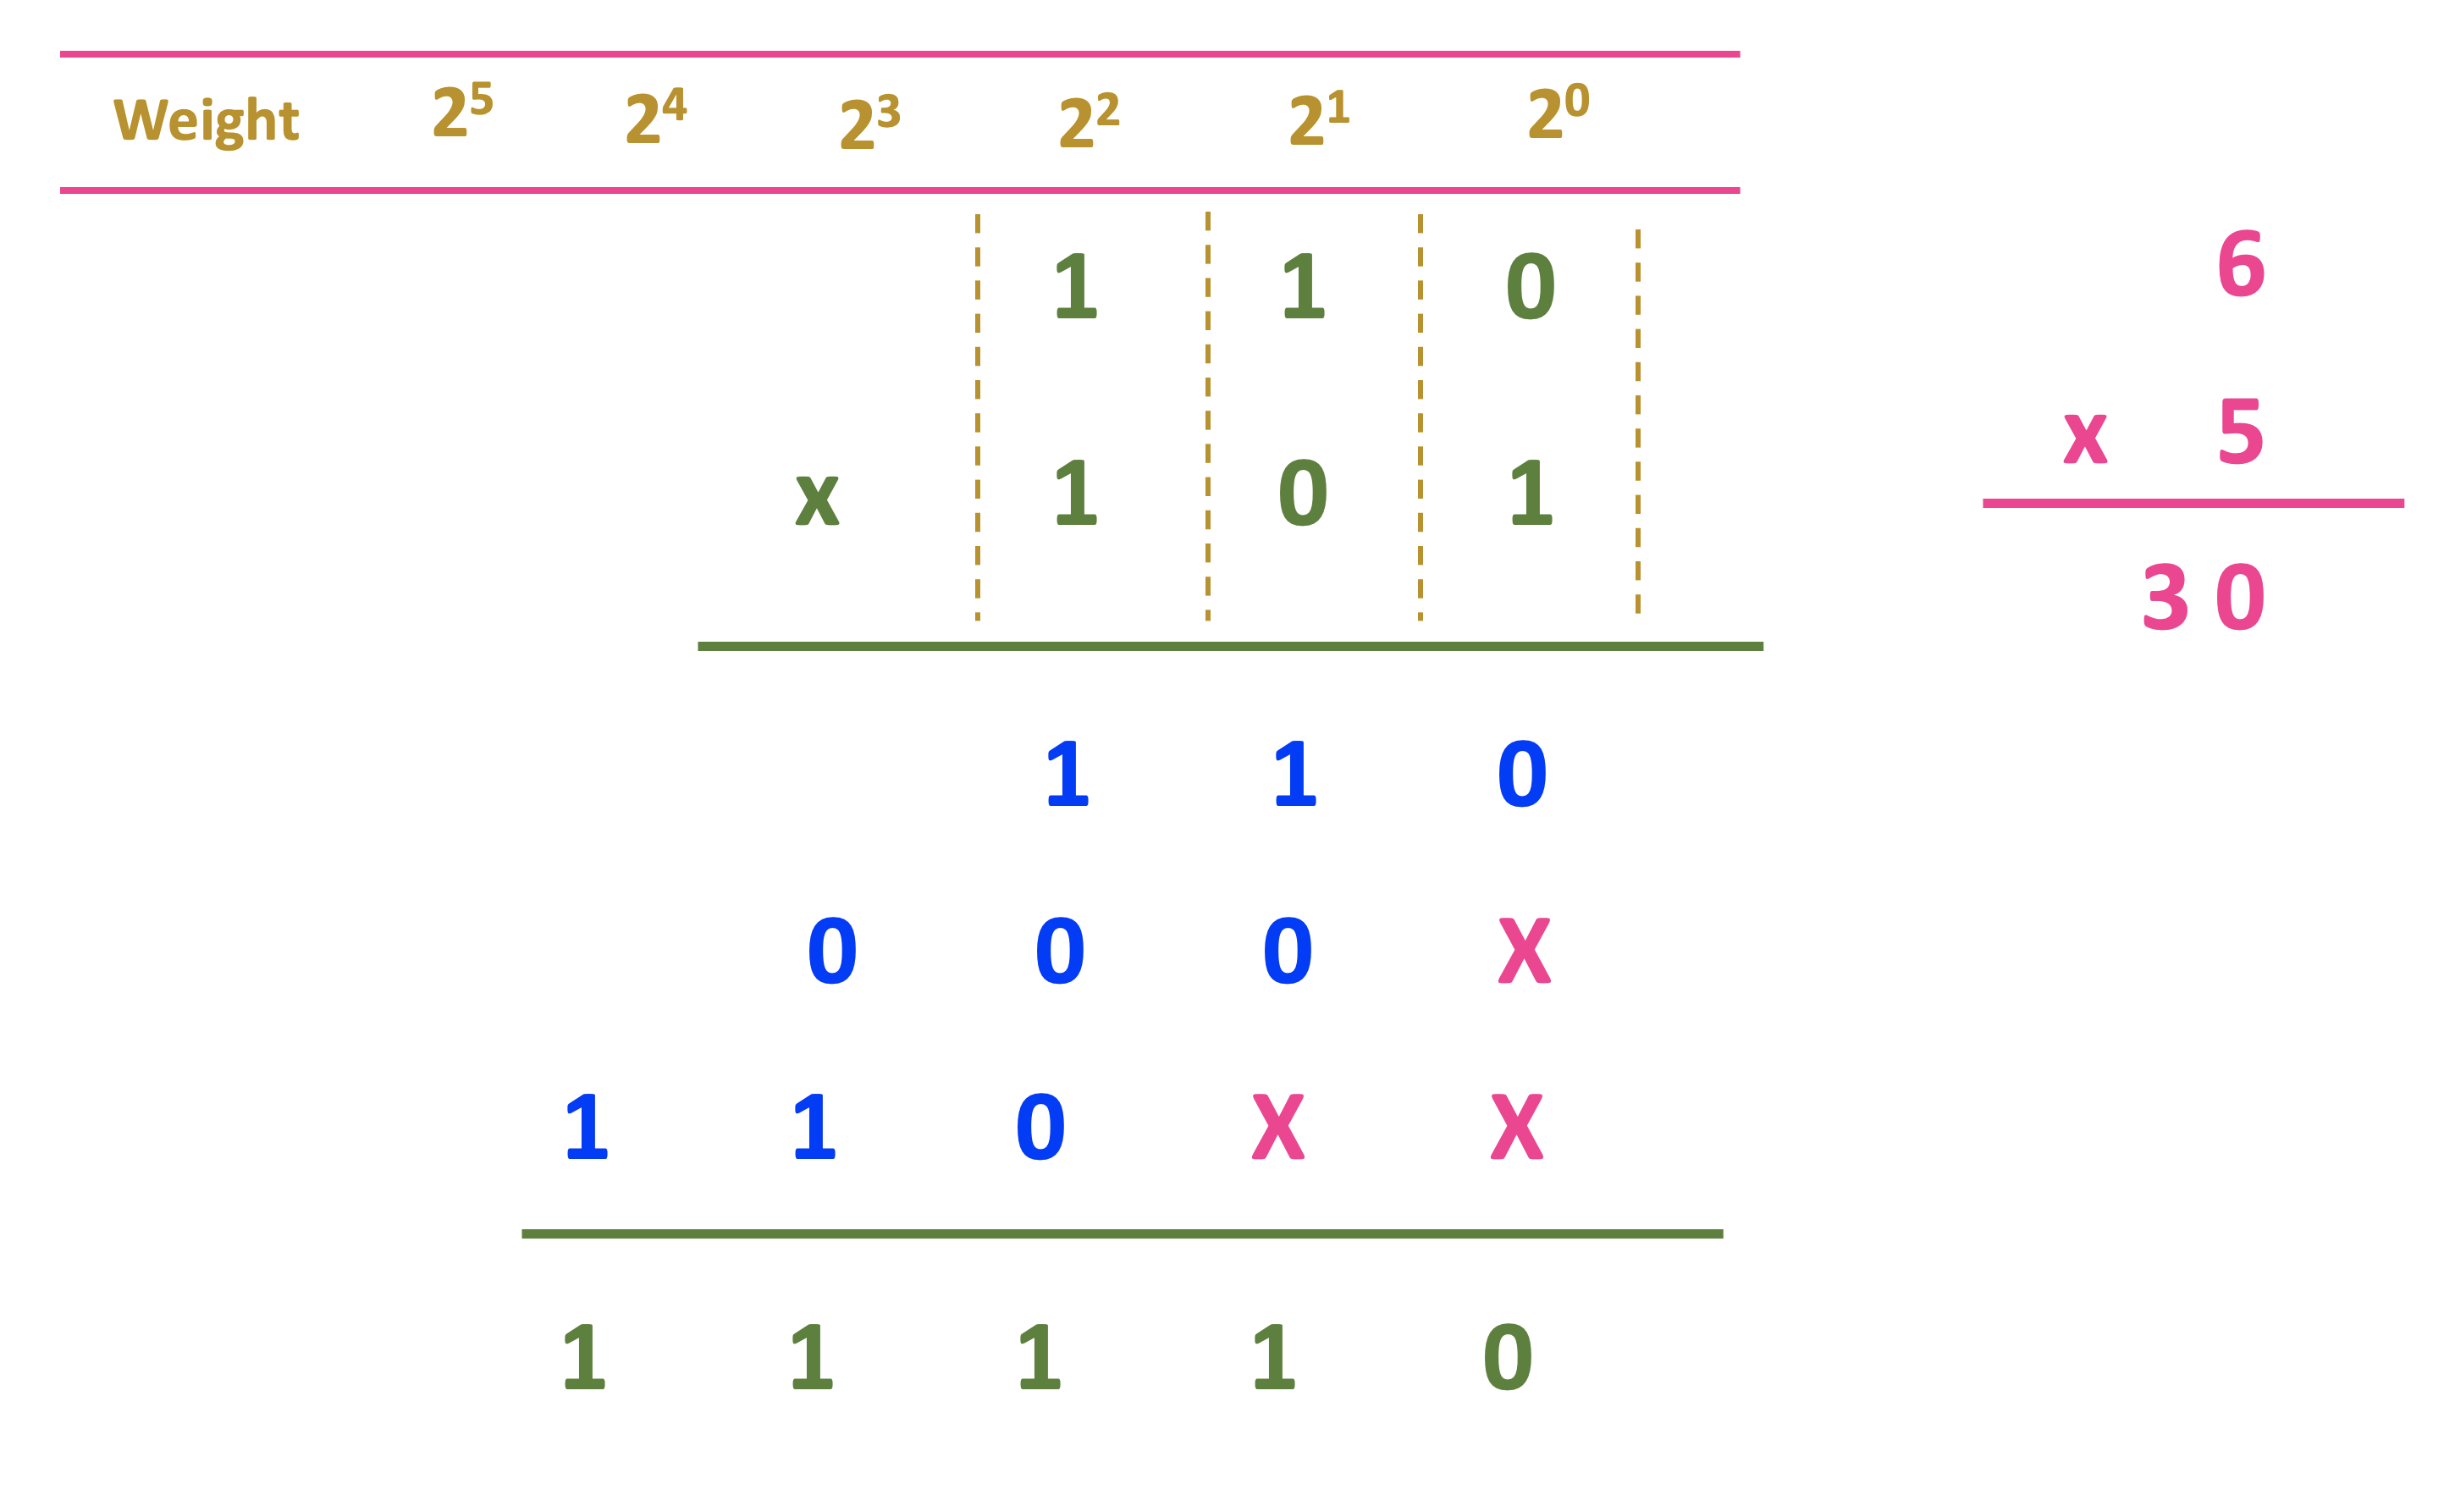
\includegraphics[width=0.8\textwidth]{figs/EM-Fig-unsigned_mul_PP.png}
    \caption{无符号乘法器中部分积生成及累加结果示意图(6$\times$5)}
    \label{EM:Fig:unsigned_mul_PP_gen}
\end{figure}




\subsubsection{补码有符号乘法器}

无符号数不能表示负数,为了解决二进制下这个问题,研究人员引入了原码(True form)、反码(1's complement)和补码(2's complement)来表示数据。
与无符号数相比,原码在最高位额外增加了一位符号位用来区分正负,0表示正数,1表示负数;在反码中,正数的反码就是其原码,负数的反码是将原码中,除符号位外,每一位按位取反;在补码中,正数的补码同样是其原码,负数的补码是其反码加一。
与原码和反码相比,补码避免了加减法不统一和存在两个零值的缺点,简化了硬件电路设计的复杂度,因此现代计算机底层采用补码的编码方式对数据进行存储和运算。
若式\eqref{EM:Eq:unsigned_fixed_Binary}为补码,$R=2$时,其最高位权重为$-2^{n-1}$,式\eqref{EM:Eq:unsigned_fixed_Decimal}变为:
% \begin{equation}
\begin{align}
    % V(A) = & \ D(A_2) \notag \\
    % = & \ ( \ \textcolor{red}{-}a_{n-1} \times R^{n-1} + a_{n-2} \times R^{n-2} + \cdots + a_1 \times R^1 + a_0 \times R^0 + \notag \\
    % & \ a_{-1} \times R^{-1} + a_{-2} \times R^{-2} + \cdots + a_{-m+1} \times R^{-m+1} + a_{-m} \times R^{-m} \ )_{10} \notag \\
    % = & \  ( \ \textcolor{red}{-}a_{n-1} \times 2^{n-1} + a_{n-2} \times 2^{n-2} + \cdots + a_1 \times 2^1 + a_0 \times 2^0 + \label{EM:Eq:signed_fixed_Decimal} \\
    % & \ a_{-1} \times 2^{-1} + a_{-2} \times 2^{-2} + \cdots + a_{-m+1} \times 2^{-m+1} + a_{-m} \times 2^{-m} \ )_{10} \notag \\
    % = & \ ( \textcolor{red}{-}a_{n-1} \times 2^{n-1} + \sum_{i=-m}^{n-2} a_i \times 2^i \ )_{10} \notag
    V(A) = & \ \textcolor{red}{-}a_{n-1}  R^{n-1} + a_{n-2}  R^{n-2} + \cdots + a_1  R^1 + a_0  R^0 + \notag \\
    & \ a_{-1}  R^{-1} + a_{-2}  R^{-2} + \cdots + a_{-m+1}  R^{-m+1} + a_{-m}  R^{-m} \notag \\
    = & \ \textcolor{red}{-}a_{n-1}  2^{n-1} + a_{n-2}  2^{n-2} + \cdots + a_1  2^1 + a_0  2^0 + \notag \\
    & \ a_{-1}  2^{-1} + a_{-2}  2^{-2} + \cdots + a_{-m+1}  2^{-m+1} + a_{-m}  2^{-m} \notag \\
    = & \ \textcolor{red}{-}a_{n-1}  2^{n-1} + \sum_{i=-m}^{n-2} a_i  2^i
\label{EM:Eq:signed_fixed_Decimal}
\end{align}
% \end{equation}

这里$n+m \ge 2$(引入了一位符号位),$n=1$和$m=0$时分别表示补码纯小数和补码整数。若不局限于二进制,式\eqref{EM:Eq:signed_fixed_Decimal}不一定成立 \footnote{https://blog.csdn.net/mydreamongo/article/details/8863502},即$R$进制下,补码的最高位权重不一定是$-R^{n-1}$。
另外,一般地,对于一个$N$位$R$进制定点数($N$是正整数,$N \geq 2$),忽略小数点,不同编码方式能够表示的数值范围为:
% \begin{equation}
\begin{align}
    & \text{无符号数:}  & [0, \ R^N-1] \ , \\
    & \text{原码与反码:}  & [- \lfloor \frac{R^N-1}{2} \rfloor, \ \lfloor \frac{R^N-1}{2} \rfloor] \ , \\
    & \text{补码:} & [- \lceil \frac{R^N-1}{2} \rceil, \ \lfloor \frac{R^N-1}{2} \rfloor] \ .
\end{align}
% \end{equation}
式中$\lfloor \ \rfloor$和$\lceil \ \rceil$分别表示向下取整和向上取整。例如,$R=2$,$N=8$时,原码和反码的表示范围为[-127,127],补码的表示范围为[-128,127]。$R=3$,$N=4$时,原码、反码和补码的表示范围均为[-40,40]。
% \textcolor{red}{之后的内容,只要不特殊说明,均基于二进制($R=2$)。}

对于补码有符号二进制乘法器(Signed binary multiplier),目前常见的部分积生成方法有:符号位扩展、改进的Baugh–Wooley算法\cite{EM:baugh-wooley,EM:baugh-wooley_modified_PP_reorga,EM:baugh-wooley_diff}、以及基4的布斯编码\cite{EM:booth_orig,EM:booth_Macsorley,EM:booth_proof}。下面分别进行介绍:

(1)符号位扩展。

按照实现细节分类,符号位扩展方法分为两种:一种是操作数(Operand)符号位扩展,优点是硬件实现不需要支持减法,缺点是部分积的规模巨大,累加电路非常复杂;另一种是部分积符号位扩展,优点是不需要修改操作数,部分积的规模适中,缺点是需要对最后一个部分积执行减法。具体细节如下:

\begin{itemize}
    \item 操作数符号位扩展。首先根据乘数和被乘数确定乘积所需要的位宽,然后将两个操作数的位宽扩展到与乘积的位宽一致,扩展方法为高位符号位扩展,即正数进行0扩展,负数进行1扩展;之后仿照无符号数二进制乘法通过逻辑与(AND)得到部分积;最后进行累加求和,注意求和后的结果应根据乘积的正确位宽进行截断。
    \item 部分积符号位扩展。同样先确定乘积所需要的位宽,但不修改操作数,通过逻辑与(AND)得到部分积;然后对部分积进行高位符号位扩展(正数0扩展,负数1扩展),将每个部分积的位宽扩展到乘积位宽;最后对部分积进行累加,但对最后一个部分积执行减法。注意对于二进制补码来说, $-[A]_\text{补} = [-A]_\text{补}$,即可以通过“按位取反加1,符号位进位丢掉”求补码的相反数,将减法转换为加法。
\end{itemize}
% \begin{figure}[!htb]
%     \centering
%     \subfigure[操作数符号位扩展示意图。]{
%     \label{EM:Fig:操作数符号位扩展}
%     \begin{minipage}[t]{0.54\linewidth}
%     \centering
%     \includegraphics[width=\linewidth]{figs/EM:Fig:操作数符号位扩展.pdf}
%     \end{minipage}
%     }\ \ \ 
%     \subfigure[部分积符号位扩展示意图。]{
%     \label{EM:Fig:部分积符号位扩展}
%     \begin{minipage}[t]{0.4\linewidth}
%     \centering
%     \includegraphics[width=\linewidth]{figs/EM:Fig:部分积符号位扩展.pdf}
%     \end{minipage}
%     }
% \caption{补码乘法器的两种符号位扩展方法示意图}
% \label{EM:Fig:signed_mul_sign_extension}
% \end{figure}
\begin{figure}[!htb]
    \centering
    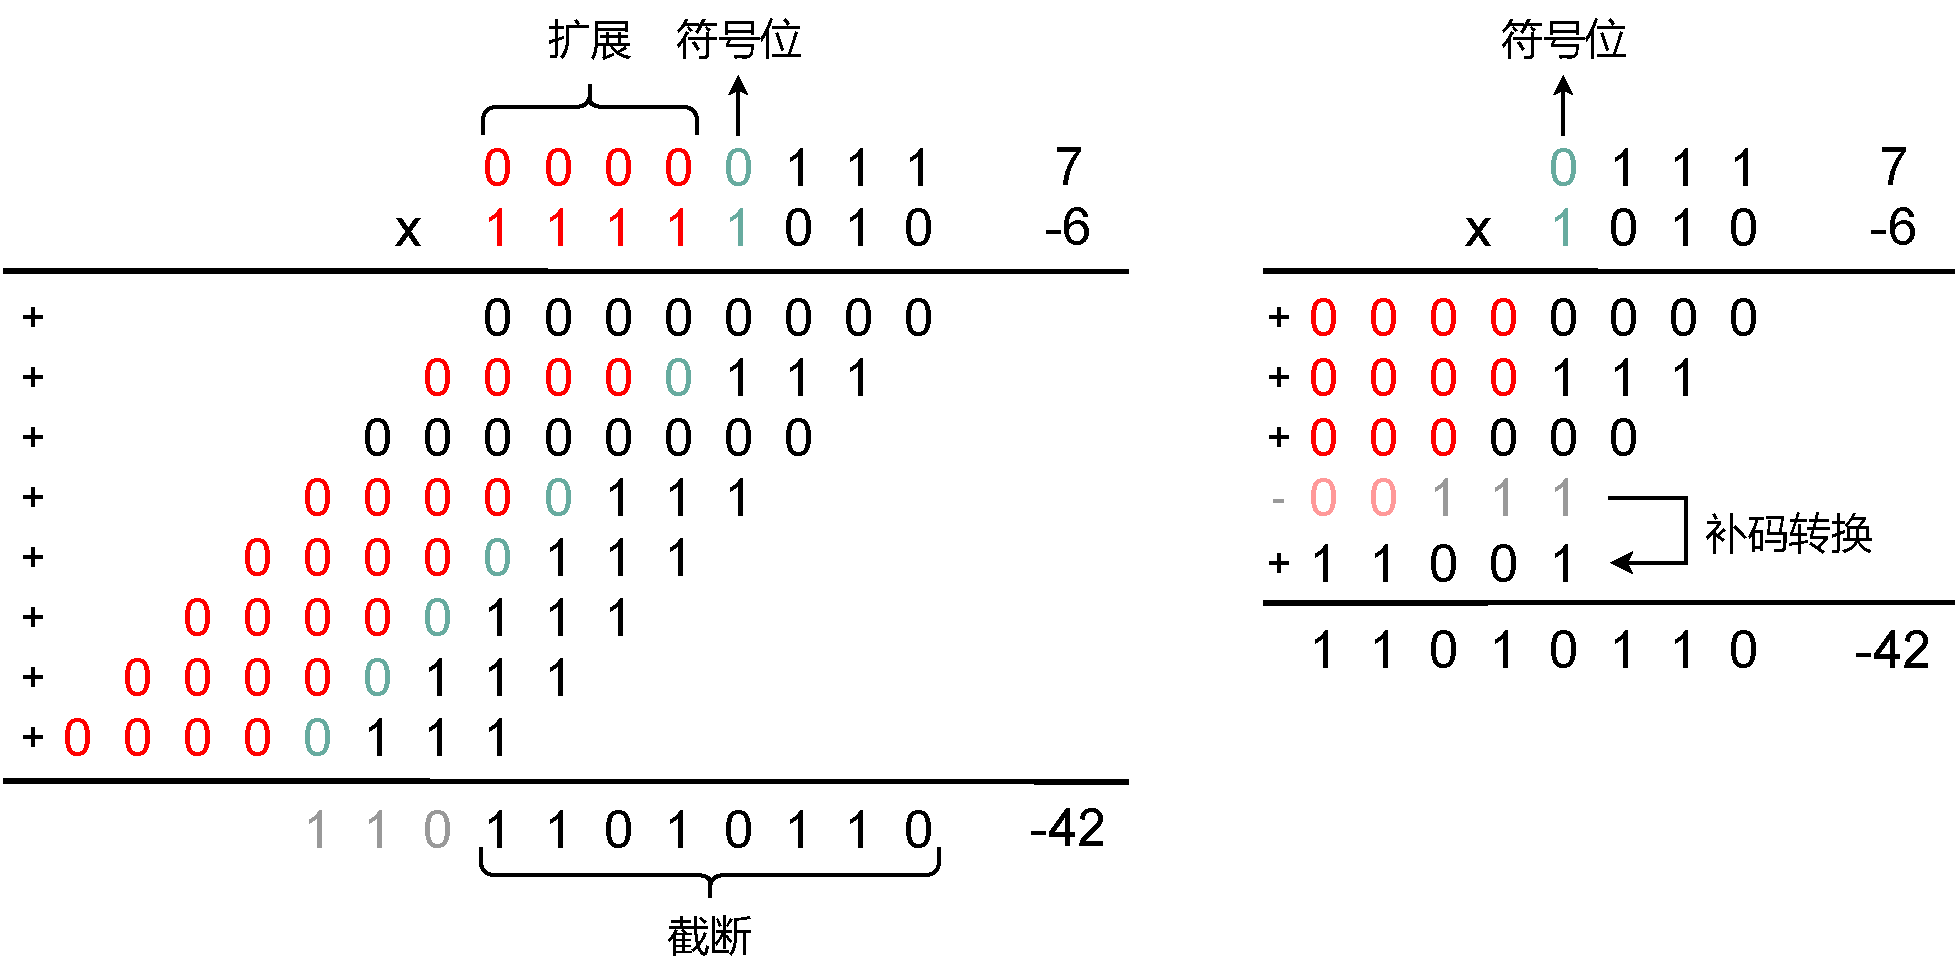
\includegraphics[width=\textwidth]{figs/EM-Fig-符号位扩展.pdf}
    \caption{补码乘法器的符号位扩展示例:左:操作数符号位扩展,右:部分积符号位扩展。}
    \label{EM:Fig:signed_mul_sign_extension}
\end{figure}

图\ref{EM:Fig:signed_mul_sign_extension}举例说明了两种符号位扩展方法的不同之处。可以看到,与操作数扩展相比,部分积扩展需要的加法更少,对应的硬件实现也更具有优势。然而,与无符号乘法相比,符号位扩展总会增大部分积的规模,使电路设计更复杂。有没有办法能够将其降低到和无符号乘法同一个水平?改进的Baugh-Wooley算法是一种解决方案\cite{EM:baugh-wooley,EM:baugh-wooley_modified_PP_reorga,EM:baugh-wooley_diff}。

(2)改进的Baugh-Wooley算法 \label{改进的Baugh-Wooley算法}

Baugh-Wooley算法是由Baugh和Wooley于1973年提出的用于二进制补码相乘的算法\cite{EM:baugh-wooley},该算法对权重为负的部分积进行修正,避免了符号位扩展,原理如下:

\noindent 设$m=0$,由式\eqref{EM:Eq:signed_fixed_Decimal}得两个$n$比特整数$X$和$Y$的十进制值:
\begin{equation}
    V(X) = -x_{n-1} 2^{n-1} + \sum_{i=0}^{n-2} x_i 2^i \ \ \ \ \ \ \ \
    V(Y) = -y_{n-1} 2^{n-1} + \sum_{i=0}^{n-2} y_i 2^i
\label{EM:Eq:signed_comp_XY}
\end{equation}
其乘积$P$:
% \begin{equation}
\begin{align}
    V(P) = & \ V(X)V(Y) \notag \\
    = & \ ( \textcolor{red}{-x_{n-1}  2^{n-1}} + \textcolor{magenta}{\sum_{i=0}^{n-2} x_i  2^i} ) \times
    ( \textcolor{blue}{-y_{n-1}  2^{n-1}} + \textcolor{cyan}{\sum_{i=0}^{n-2} y_i  2^i} ) \notag \\
%
    = & \ \textcolor{red}{x_{n-1}} \textcolor{blue}{y_{n-1}}  2^{2n-2} +
    \textcolor{magenta}{\sum_{i=0}^{n-2} x_i 2^i} \textcolor{cyan}{\sum_{j=0}^{n-2} y_j 2^j}
    \textcolor{red}{-x_{n-1}  2^{n-1}} \textcolor{cyan}{\sum_{i=0}^{n-2} y_i  2^i}
    \textcolor{blue}{-y_{n-1}  2^{n-1}} \textcolor{magenta}{\sum_{i=0}^{n-2} x_i  2^i} \notag \\
%
    = & \ \textcolor{red}{x_{n-1}} \textcolor{blue}{y_{n-1}}  2^{2n-2} +
    \textcolor{magenta}{\sum_{i=0}^{n-2}} \textcolor{cyan}{\sum_{j=0}^{n-2}} \textcolor{magenta}{x_i} \textcolor{cyan}{y_j} 2^{\textcolor{magenta}{i}+\textcolor{cyan}{j}} 
    \textcolor{red}{-2^{n-1}} \textcolor{cyan}{\sum_{i=0}^{n-2}} \textcolor{red}{x_{n-1}} \textcolor{cyan}{y_i 2^i}
    \textcolor{blue}{-2^{n-1}} \textcolor{magenta}{\sum_{i=0}^{n-2}} \textcolor{blue}{y_{n-1}} \textcolor{magenta}{x_i 2^i}
\label{EM:Eq:signed_comp_P}
\end{align}
% \end{equation}
$n=5$时,式\eqref{EM:Eq:signed_comp_P}对应的部分积阵列如图\ref{EM:Fig:signed_mul_PP_array}所示,其中红色部分积的权重为负数,对应式\eqref{EM:Eq:signed_comp_P}中的后两项:
\begin{figure}[!htb]
    \centering
    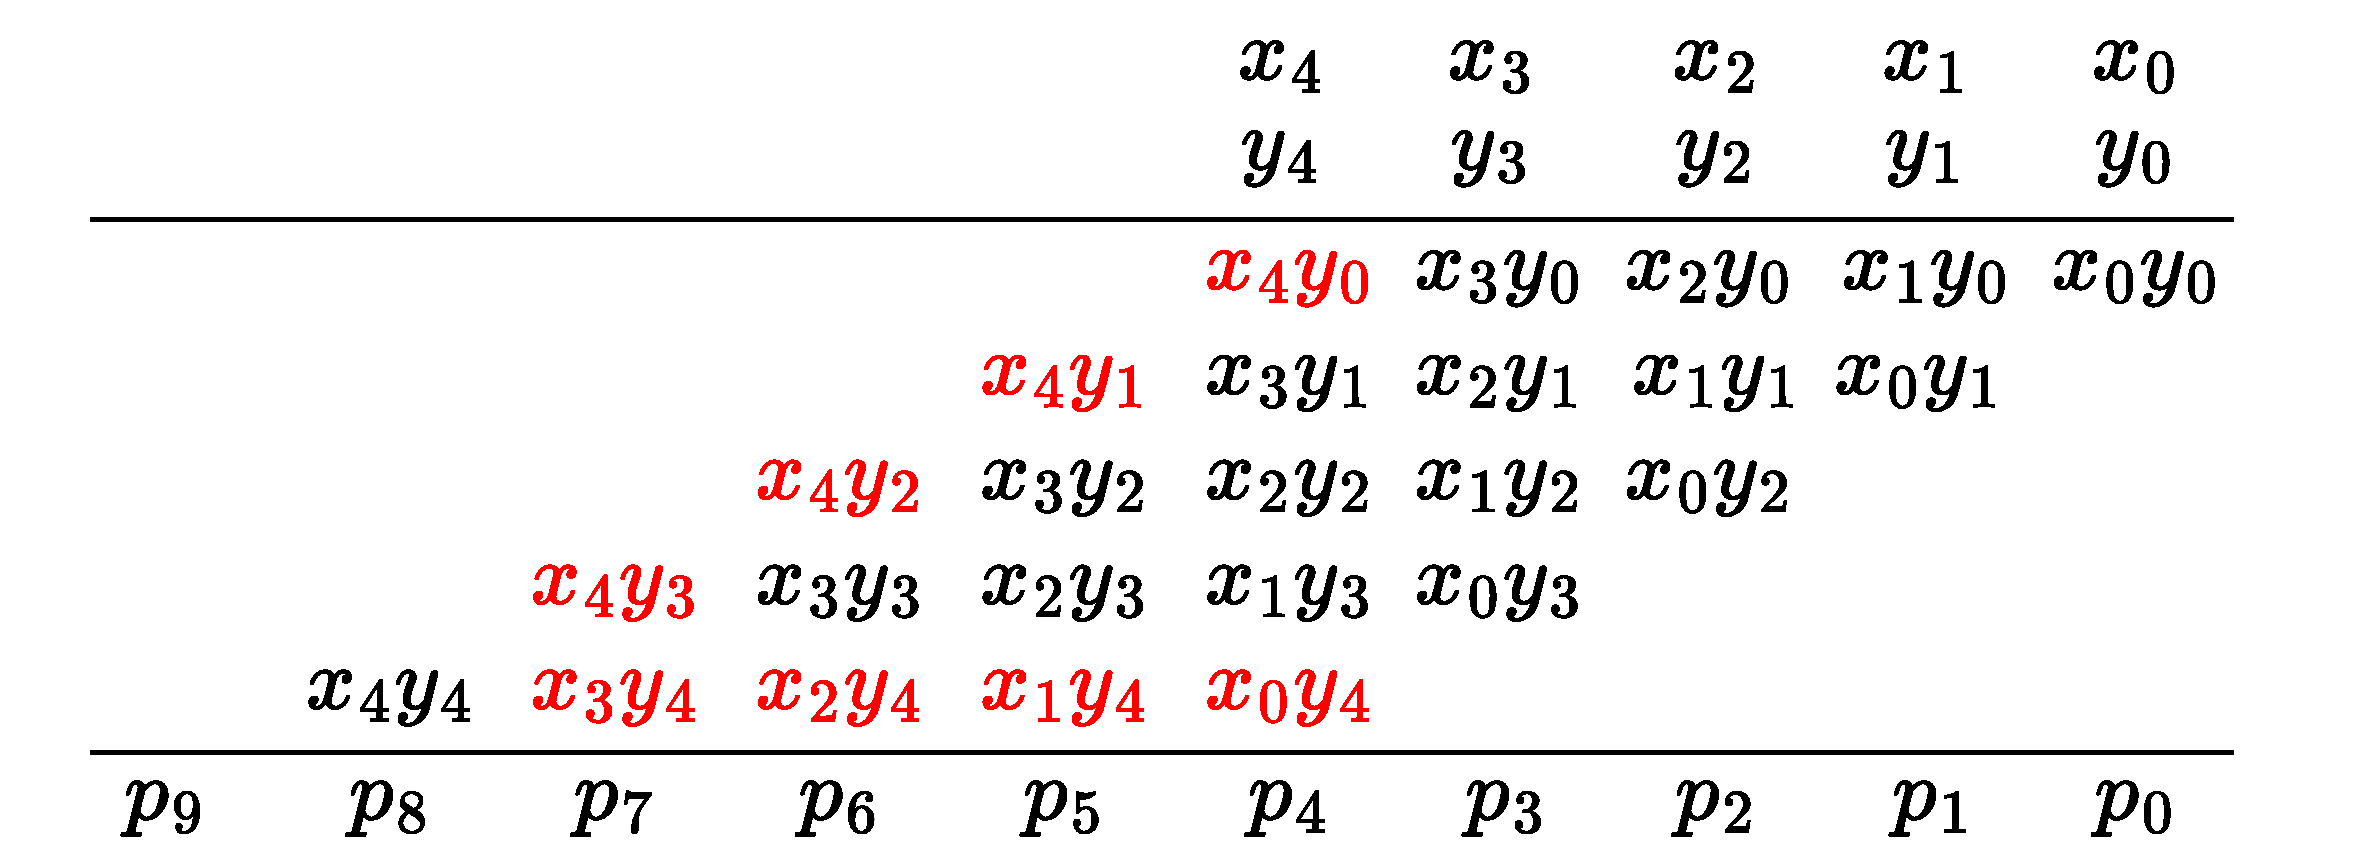
\includegraphics[width=0.85\textwidth]{figs/EM-Fig-补码部分积阵列.pdf}
    \caption{$5 \times 5$补码乘法器的部分积阵列示意图,红色部分积的权重为负}
    \label{EM:Fig:signed_mul_PP_array}
\end{figure}

\noindent 对于任一补码(不失一般性,假设是式\eqref{EM:Eq:signed_comp_XY}中的$X$):
\begin{equation}
    -V(X) = - \overline {x_{n-1}} 2^{n-1} + \sum_{i=0}^{n-2} \overline{x_i} 2^i +1 \ \ \text{(按位取反加1,符号位进位丢掉)}
    \label{EM:Eq:signed_comp_subtract}
\end{equation}
式\eqref{EM:Eq:signed_comp_P}中的后两项变为:
% \begin{equation}
\begin{align}
& \textcolor{red}{-2^{n-1}} ( -0 \cdot 2^n + 0 \cdot 2^{n-1} + \textcolor{cyan}{\sum_{i=0}^{n-2}} \textcolor{red}{x_{n-1}} \textcolor{cyan}{y_i 2^i} )
\textcolor{blue}{-2^{n-1}} ( -0 \cdot 2^n + 0 \cdot 2^{n-1} + \textcolor{magenta}{\sum_{i=0}^{n-2}} \textcolor{blue}{y_{n-1}} \textcolor{magenta}{x_i 2^i} ) \notag \\
%
= & \textcolor{red}{+2^{n-1}} ( -1 \cdot 2^n + 1 \cdot 2^{n-1} + \textcolor{cyan}{\sum_{i=0}^{n-2}} \overline{ \textcolor{red}{x_{n-1}}  \textcolor{cyan}{y_i}}  \textcolor{cyan}{2^i} + 1 ) \
\textcolor{blue}{+2^{n-1}} ( -1 \cdot 2^n + 1 \cdot 2^{n-1} + \textcolor{magenta}{\sum_{i=0}^{n-2}} \overline{ \textcolor{blue}{y_{n-1}}  \textcolor{magenta}{x_i} } \textcolor{magenta}{2^i} + 1 ) \label{EM:Eq:signed_comp_P_Baugh-Wooley_positve}
\end{align}

\noindent 为了避免出现与非门(NAND),注意到式\eqref{EM:Eq:signed_comp_P_Baugh-Wooley_positve}第一项为:
\begin{equation}
    \left\{
    \begin{aligned}
        \ & 0 , & \ \ x_{n-1} = 0, \\
        \ & \textcolor{red}{+2^{n-1}} ( - 2^n + 2^{n-1} + \textcolor{cyan}{\sum_{i=0}^{n-2}} \overline{ \textcolor{cyan}{y_i}}  \textcolor{cyan}{2^i} + 1 ), & \ \ x_{n-1} = 1.
    \end{aligned}
    \right.
\end{equation}
即:
\begin{equation}
    \textcolor{red}{+2^{n-1}} ( - 2^n + 2^{n-1} + \overline{x_{n-1}} 2^{n-1} + x_{n-1} + \textcolor{cyan}{\sum_{i=0}^{n-2}} x_{n-1} \overline{ \textcolor{cyan}{y_i}}  \textcolor{cyan}{2^i} )
\label{EM:Eq:signed_comp_P_Baugh-Wooley_rNAND_x}
\end{equation}
同理式\eqref{EM:Eq:signed_comp_P_Baugh-Wooley_positve}第二项为:
\begin{equation}
    \left\{
    \begin{aligned}
        \ & 0 , & \ \ y_{n-1} = 0, \\
        \ & \textcolor{blue}{+2^{n-1}} ( - 2^n + 2^{n-1} + \textcolor{magenta}{\sum_{i=0}^{n-2}} \overline{ \textcolor{magenta}{x_i} } \textcolor{magenta}{2^i} + 1 ), & \ \ y_{n-1} = 1.
    \end{aligned}
    \right.
\end{equation}
即:
\begin{equation}
    \textcolor{blue}{+2^{n-1}} ( - 2^n + 2^{n-1} + \overline{y_{n-1}} 2^{n-1} + y_{n-1} + \textcolor{magenta}{\sum_{i=0}^{n-2}} y_{n-1} \overline{ \textcolor{magenta}{x_i} } \textcolor{magenta}{2^i} )
\label{EM:Eq:signed_comp_P_Baugh-Wooley_rNAND_y}
\end{equation}
结合式\eqref{EM:Eq:signed_comp_P}、式\eqref{EM:Eq:signed_comp_P_Baugh-Wooley_positve}、式\eqref{EM:Eq:signed_comp_P_Baugh-Wooley_rNAND_x}和式\eqref{EM:Eq:signed_comp_P_Baugh-Wooley_rNAND_y},$V(P)$变为:
\begin{equation}
\begin{aligned}
    V(P) = & \ \textcolor{red}{x_{n-1}} \textcolor{blue}{y_{n-1}}  2^{2n-2} +
    \textcolor{magenta}{\sum_{i=0}^{n-2}} \textcolor{cyan}{\sum_{j=0}^{n-2}} \textcolor{magenta}{x_i} \textcolor{cyan}{y_j} 2^{\textcolor{magenta}{i}+\textcolor{cyan}{j}} \\
%
    & \ \textcolor{red}{+2^{n-1}} ( - 2^n + 2^{n-1} + \overline{x_{n-1}} 2^{n-1} + x_{n-1} + \textcolor{cyan}{\sum_{i=0}^{n-2}} x_{n-1} \overline{ \textcolor{cyan}{y_i}}  \textcolor{cyan}{2^i} ) \\
%
    & \ \textcolor{blue}{+2^{n-1}} ( - 2^n + 2^{n-1} + \overline{y_{n-1}} 2^{n-1} + y_{n-1} + \textcolor{magenta}{\sum_{i=0}^{n-2}} y_{n-1} \overline{ \textcolor{magenta}{x_i} } \textcolor{magenta}{2^i} )
\end{aligned}
\label{EM:Eq:signed_comp_P_Baugh-Wooley}
\end{equation}
式\eqref{EM:Eq:signed_comp_P_Baugh-Wooley}被称为Baugh-Wooley算法,$n=5$时,该算法对应的部分积阵列如图\ref{EM:Fig:orig_Baugh-Wooley_PP}所示,所有比特权重均为正值(除了最高位的1)。与无符号乘法器相比,不论$n$多大,由式\eqref{EM:Eq:signed_comp_P_Baugh-Wooley}得到的部分积阵列只会多5个比特。然而,原始的Baugh-Wooley方法会导致部分积阵列增加两层,不利于后面的累加,注意到式\eqref{EM:Eq:signed_comp_P_Baugh-Wooley_positve}可变为:
\begin{equation}
\textcolor{red}{+2^{n-1}}  \textcolor{cyan}{\sum_{i=0}^{n-2}} \overline{ \textcolor{red}{x_{n-1}}  \textcolor{cyan}{y_i}}  \textcolor{cyan}{2^i}
\textcolor{blue}{+2^{n-1}} \textcolor{magenta}{\sum_{i=0}^{n-2}} \overline{ \textcolor{blue}{y_{n-1}}  \textcolor{magenta}{x_i} } \textcolor{magenta}{2^i} + 1 \cdot 2^n -1 \cdot 2^{2n-1}
\label{EM:Eq:signed_comp_P_Baugh-Wooley_modified}
\end{equation}
Hatamian等人根据式\eqref{EM:Eq:signed_comp_P_Baugh-Wooley_modified}对部分积进行了重新排列\cite{EM:baugh-wooley_modified_PP_reorga},得到了\ref{EM:Fig:modified_Baugh-Wooley_PP},被称为改进的Baugh-Wooley算法\footnote{https://zhuanlan.zhihu.com/p/343133392}。改进后的Baugh-Wooley方法只在部分积引入两个1,不增加部分积阵列的层数,得到了广泛的应用\cite{EM:baugh-wooley_diff}。

\begin{figure}[!htb]
    \centering
    \subfigure[原始的Baugh-Wooley乘法器部分积阵列]{
    \label{EM:Fig:orig_Baugh-Wooley_PP}
    \begin{minipage}[t]{0.48\linewidth}
    \centering
    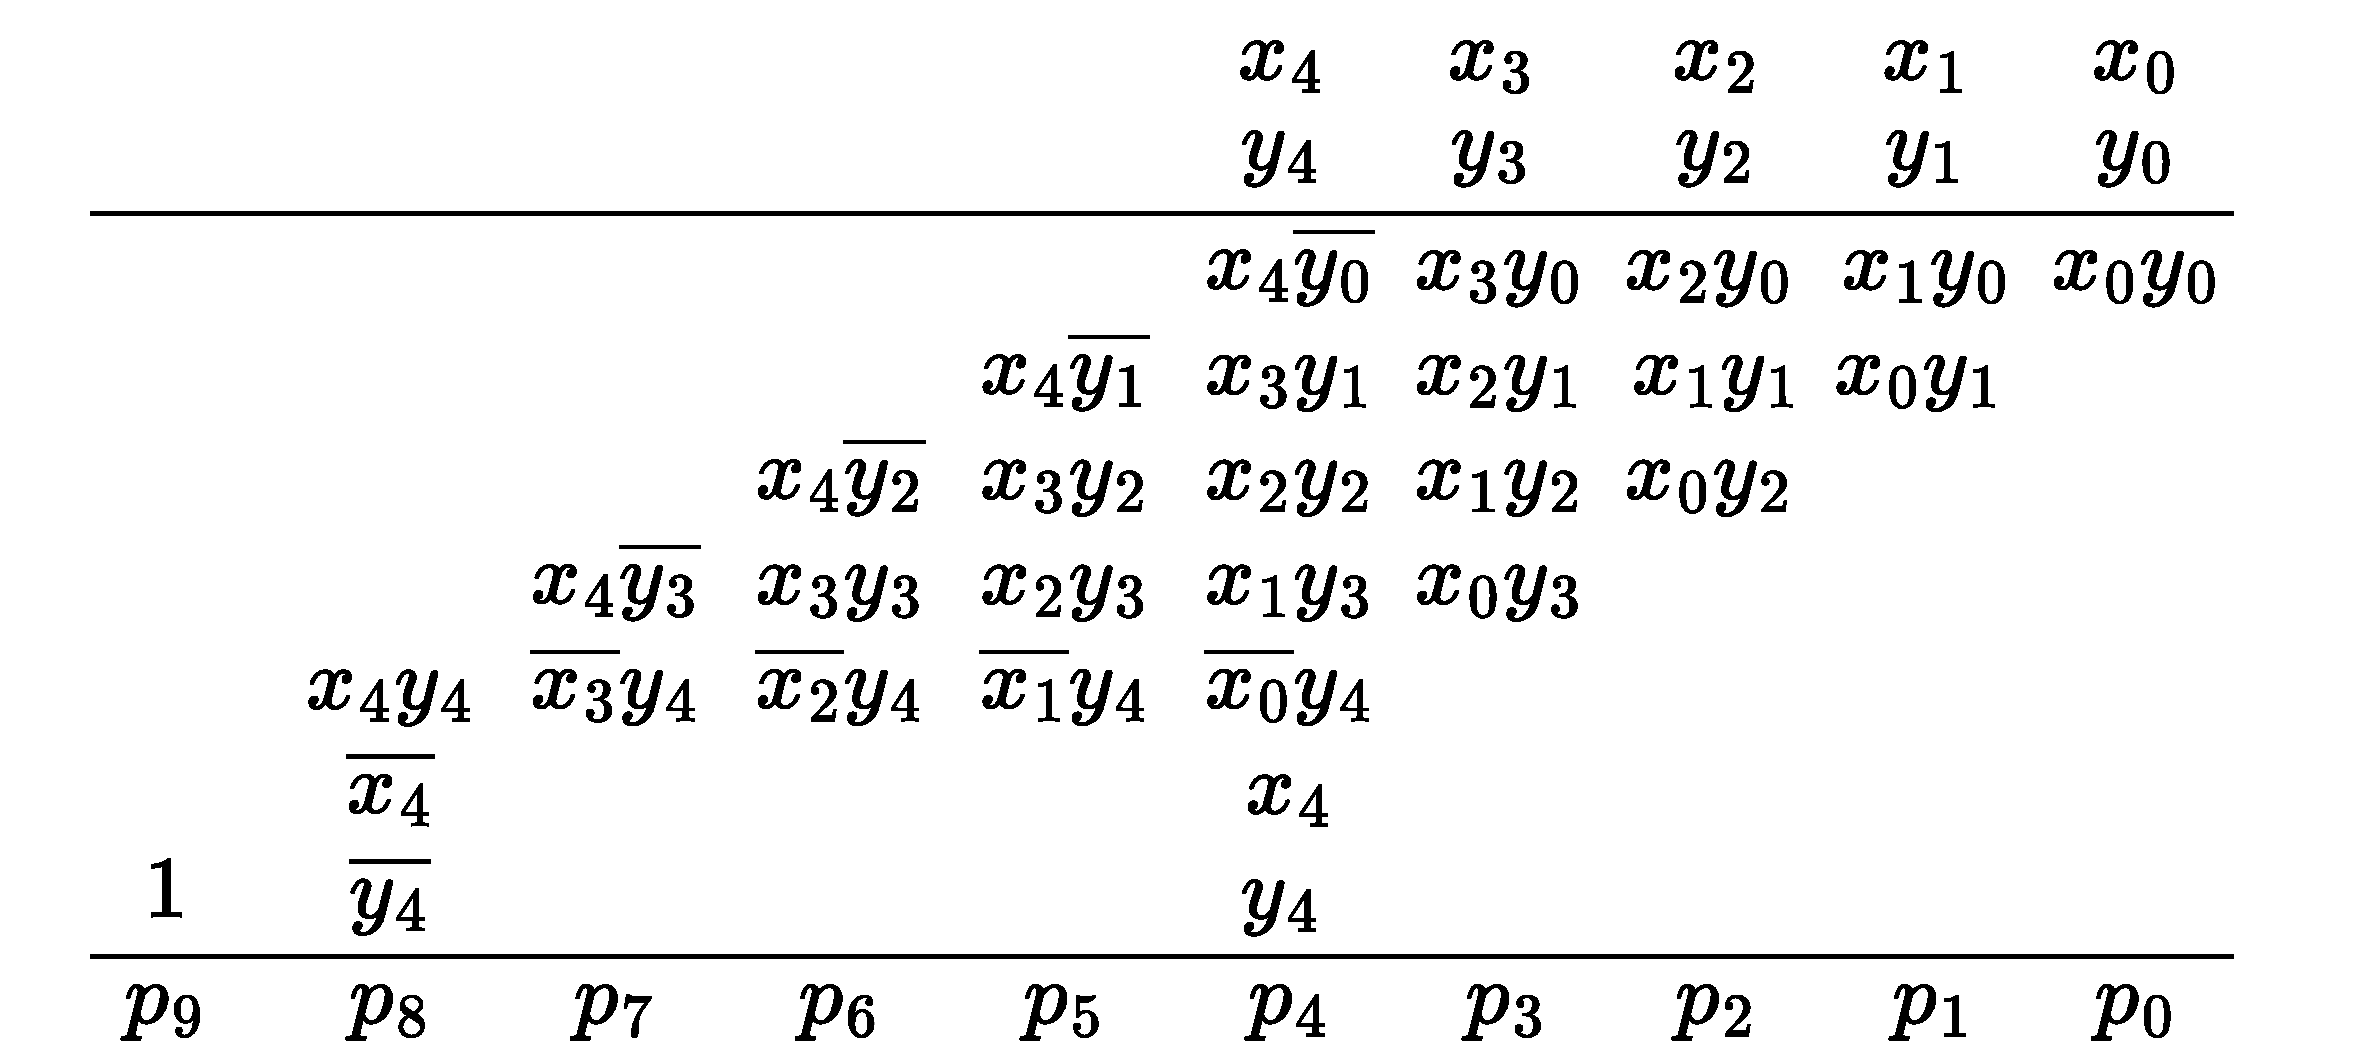
\includegraphics[width=\linewidth]{figs/EM-Fig-Baugh-Wooley.pdf}
    \end{minipage}
    }
    \subfigure[改进的Baugh-Wooley乘法器部分积阵列]{
    \label{EM:Fig:modified_Baugh-Wooley_PP}
    \begin{minipage}[t]{0.48\linewidth}
    \centering
    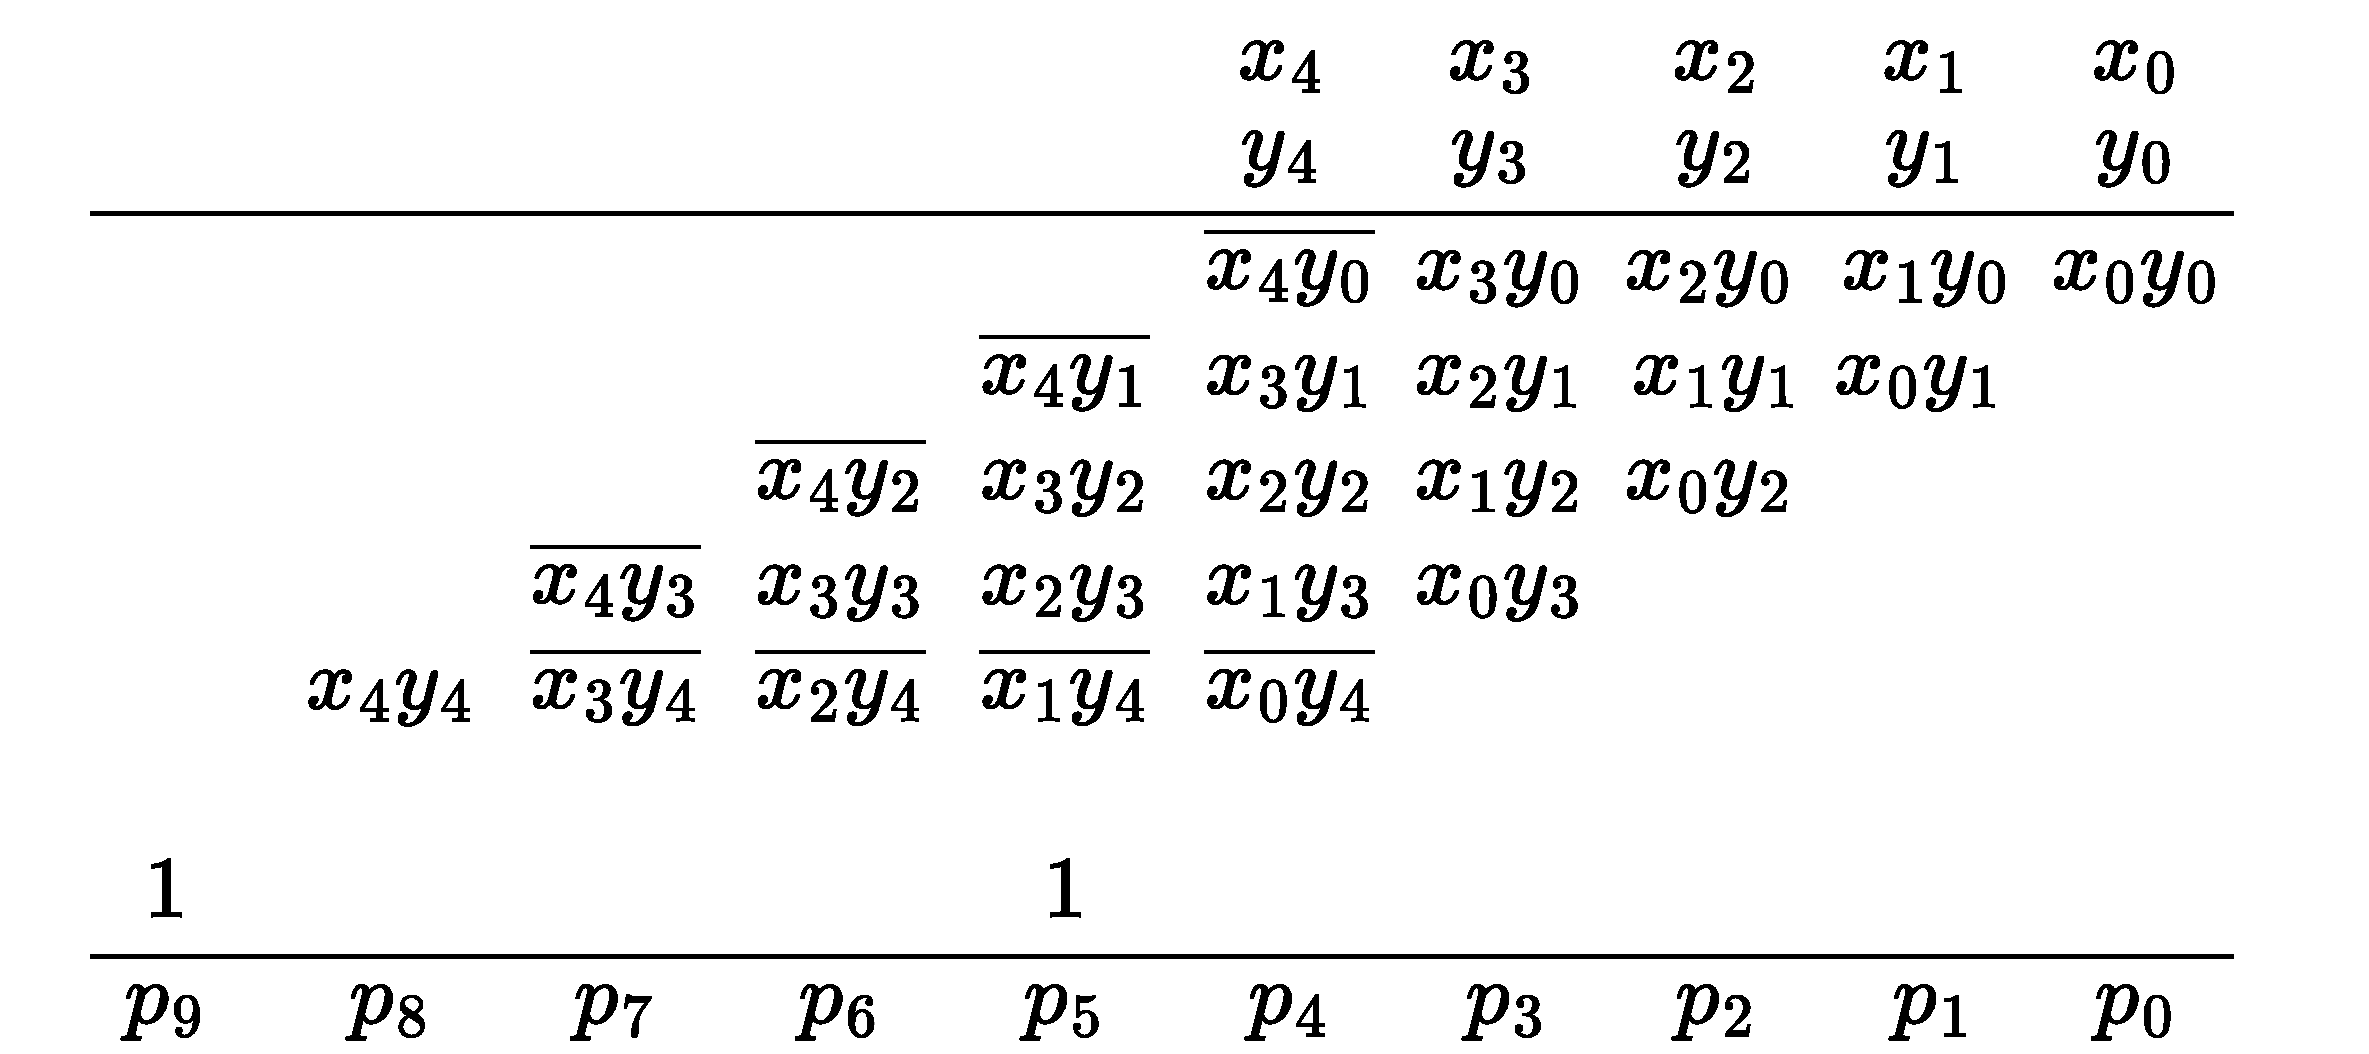
\includegraphics[width=\linewidth]{figs/EM-Fig-改进的Baugh-Wooley.pdf}
    \end{minipage}
    }
\caption{基于Baugh-Wooley算法设计的$5 \times 5$补码乘法器部分积阵列示意图}
\label{EM:Fig:signed_comp_P_Baugh-Wooley}
\end{figure}

(3)基4的布斯编码

与Baugh-Wooley算法不同,布斯编码的意义在于能够减少乘法器中部分积的个数(行数),且基数越高效果越明显,比如基4和基8的布斯编码分别能够将部分积的个数降低一半和三分之二\cite{EM:booth_Macsorley,EM:booth_proof},大大减轻后续累加的压力。然而,高基的布斯编码电路实现复杂,目前最常用的基数是4。原理如下:

对于补码有符号乘法,假设$n$为偶数,$y_{-1} = 0$,式\eqref{EM:Eq:signed_comp_XY}中的$V(Y)$变为:
\begin{align}
    V(Y) = & \ - y_{n-1} 2^{n-1} + y_{n-2} 2^{n-2} + y_{n-3} 2^{n-3} + y_{n-4} 2^{n-4} + y_{n-5} 2^{n-5} + \cdots + \notag \\
%
    & y_5 2^5 + y_4 2^4 + y_3 2^3 + y_2 2^2 + y_1 2^1 + y_0 2^0 + \textcolor{red}{y_{-1} 2^{-1}} \notag \\
%
    = & \ ( -2 y_{n-1} + y_{n-2} + y_{n-3}) 2^{n-2} + (-2 y_{n-3} + y_{n-4} + y_{n-5}) 2^{n-4} + \cdots + \notag \\
%
    & \ (-2 y_5 + y_4 + y_3) 2^4 + (-2 y_3 + y_2 + y_1) 2^2 + (-2 y_1 + y_0 + \textcolor{red}{y_{-1}} ) 2^0
\label{EM:Eq:Radix-4-booth_VY}
\end{align}
式\eqref{EM:Eq:signed_comp_P}变为:
\begin{align}
    V(P) = & \ V(X)V(Y) \notag \\
    = & \ V(X) ( -2 y_{n-1} + y_{n-2} + y_{n-3}) 2^{n-2} + \notag \\
%
    & \ V(X) (-2 y_{n-3} + y_{n-4} + y_{n-5}) 2^{n-4} + \cdots + \notag \\
%
    & \ V(X) (-2 y_5 + y_4 + y_3) 2^4 + \notag \\
    & \ V(X) (-2 y_3 + y_2 + y_1) 2^2 + \notag \\
    & \ V(X) (-2 y_1 + y_0 + \textcolor{red}{y_{-1}} ) 2^0
    \label{EM:Eq:Radix-4-booth}
\end{align}

式\eqref{EM:Eq:Radix-4-booth}是基4的布斯编码算法公式,其中$X$是被乘数,$Y$是乘数,对应的编码规则及部分积操作如表\ref{EM:Tab:Radix-4-booth}所示。该算法在进行前需要在乘数的最右侧隐含地补一个0,之后从最低有效位开始每次扫描3位乘数生成部分积,共$\dfrac{n}{2}$个,然后对部分积进行符号位扩展、累加并最终相加。由表\ref{EM:Tab:Radix-4-booth}可以看出,基4的布斯算法只涉及加法、减法和移位操作,硬件实现友好。需要注意的是,式\eqref{EM:Eq:Radix-4-booth}表示的基于补码乘法的基4布斯算法仅适用于$n$是偶数的情况,若$n$是奇数,先对乘数进行一位符号位扩展,将位宽变为偶数,之后再进行编码,部分积总数为$\dfrac{n+1}{2}$个。布斯编码得到的部分积仍然需要符号位扩展,一个直接的方法是首先根据被乘数和乘数确定乘积位宽,然后直接通过高位符号位扩展将每个部分积的位宽增加到乘积位宽,但这种方法产生的部分积规模较大,累加电路复杂,可采用改进的符号位扩展方法对其进行优化。

\begin{table}
\centering
\caption{基4布斯编码表}
\begin{tabular}{|c|c|c|c|c|} \hline
$y_{i+1}$ & $y_i$ & $y_{i-1}$ & $-2 y_{i+1} + y_i + y_{i-1}$ & \text{部分积操作} \\ \hline
0 & 0 & 0 & 0 & +0 \\ \hline
0 & 0 & 1 & 1 & $+[X]_{\text{补}}$ \\ \hline
0 & 1 & 0 & 1 & $+[X]_{\text{补}}$ \\ \hline
0 & 1 & 1 & 2 & $+2[X]_{\text{补}}$ \\ \hline
1 & 0 & 0 & -2 & $-2[X]_{\text{补}}$ \\ \hline
1 & 0 & 1 & -1 & $-[X]_{\text{补}}$ \\ \hline
1 & 1 & 0 & -1 & $-[X]_{\text{补}}$ \\ \hline
1 & 1 & 1 & 0 & +0 \\ \hline
\end{tabular}
\label{EM:Tab:Radix-4-booth}
\end{table}

另外,布斯算法也可以用于无符号数乘法\footnote{https://picture.iczhiku.com/resource/eetop/whKDFaTwqTZOkCxn.pdf},为了支持布斯编码中需要的减法操作,部分积也应采用补码格式。若基数取4,编码形式仍然是$-2 y_{i+1} + y_i + y_{i-1}$,与补码乘法的基4布斯算法的区别在于:(a)$n$是偶数时需要添加的不仅是$y_{-1} = 0$,还有$y_{n+1} = y_n = 0$,此时$\{y_{n+1}, y_n, y_{n-1} \}$编码得到的部分积一定是0或正数,部分积总数为$\dfrac{n}{2} + 1$个;(b)$n$是奇数时需要添加的是$y_n = y_{-1} = 0$ ,部分积总数为$\dfrac{n+1}{2}$个;(c)优化后的符号位扩展方法实现细节略微不同。

下面具体讲解基4布斯算法在无符号数乘法和补码有符号数乘法中部分积符号位扩展方法优化细节的不同\cite{EM:booth_sign_extension}:


\begin{figure}[!htb]
    \centering
    \subfigure[部分积均为正数,省略了高位的0扩展]{
    \label{EM:Fig:booth_16x16_unsign_PP_positive}
    \begin{minipage}[t]{0.48\linewidth}
    \centering
    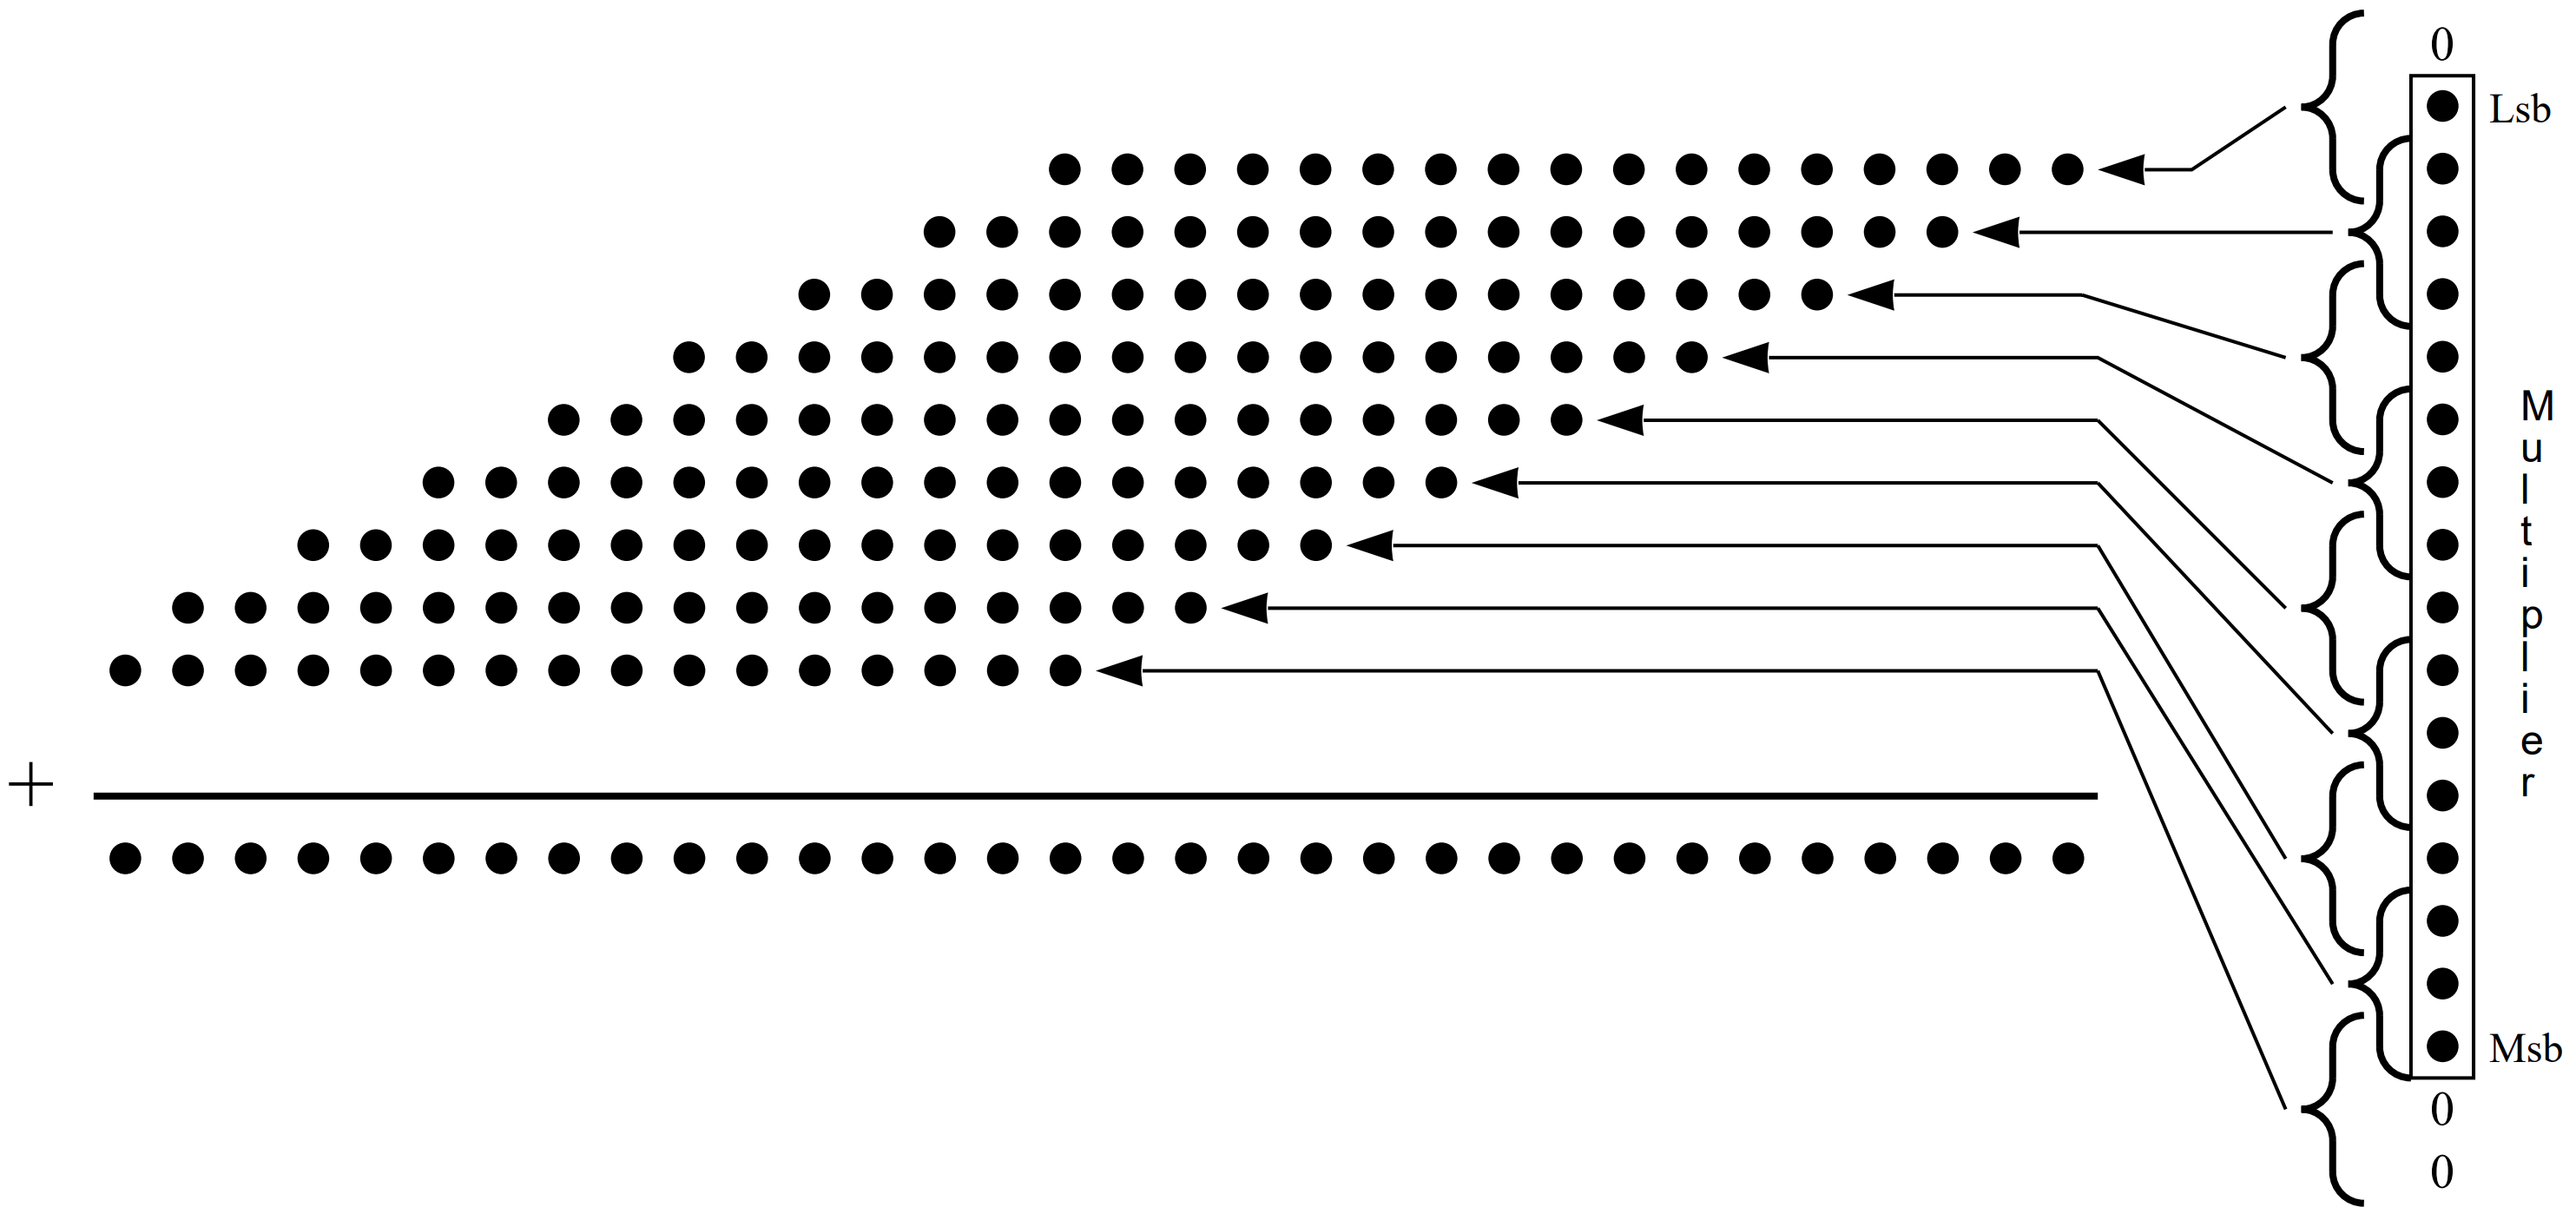
\includegraphics[width=\linewidth]{figs/EM-Fig-booth_unsign_positive.png}
    \end{minipage}
    }
    \subfigure[部分积均为负数,高位进行1扩展]{
    \label{EM:Fig:booth_16x16_unsign_PP_negtive}
    \begin{minipage}[t]{0.48\linewidth}
    \centering
    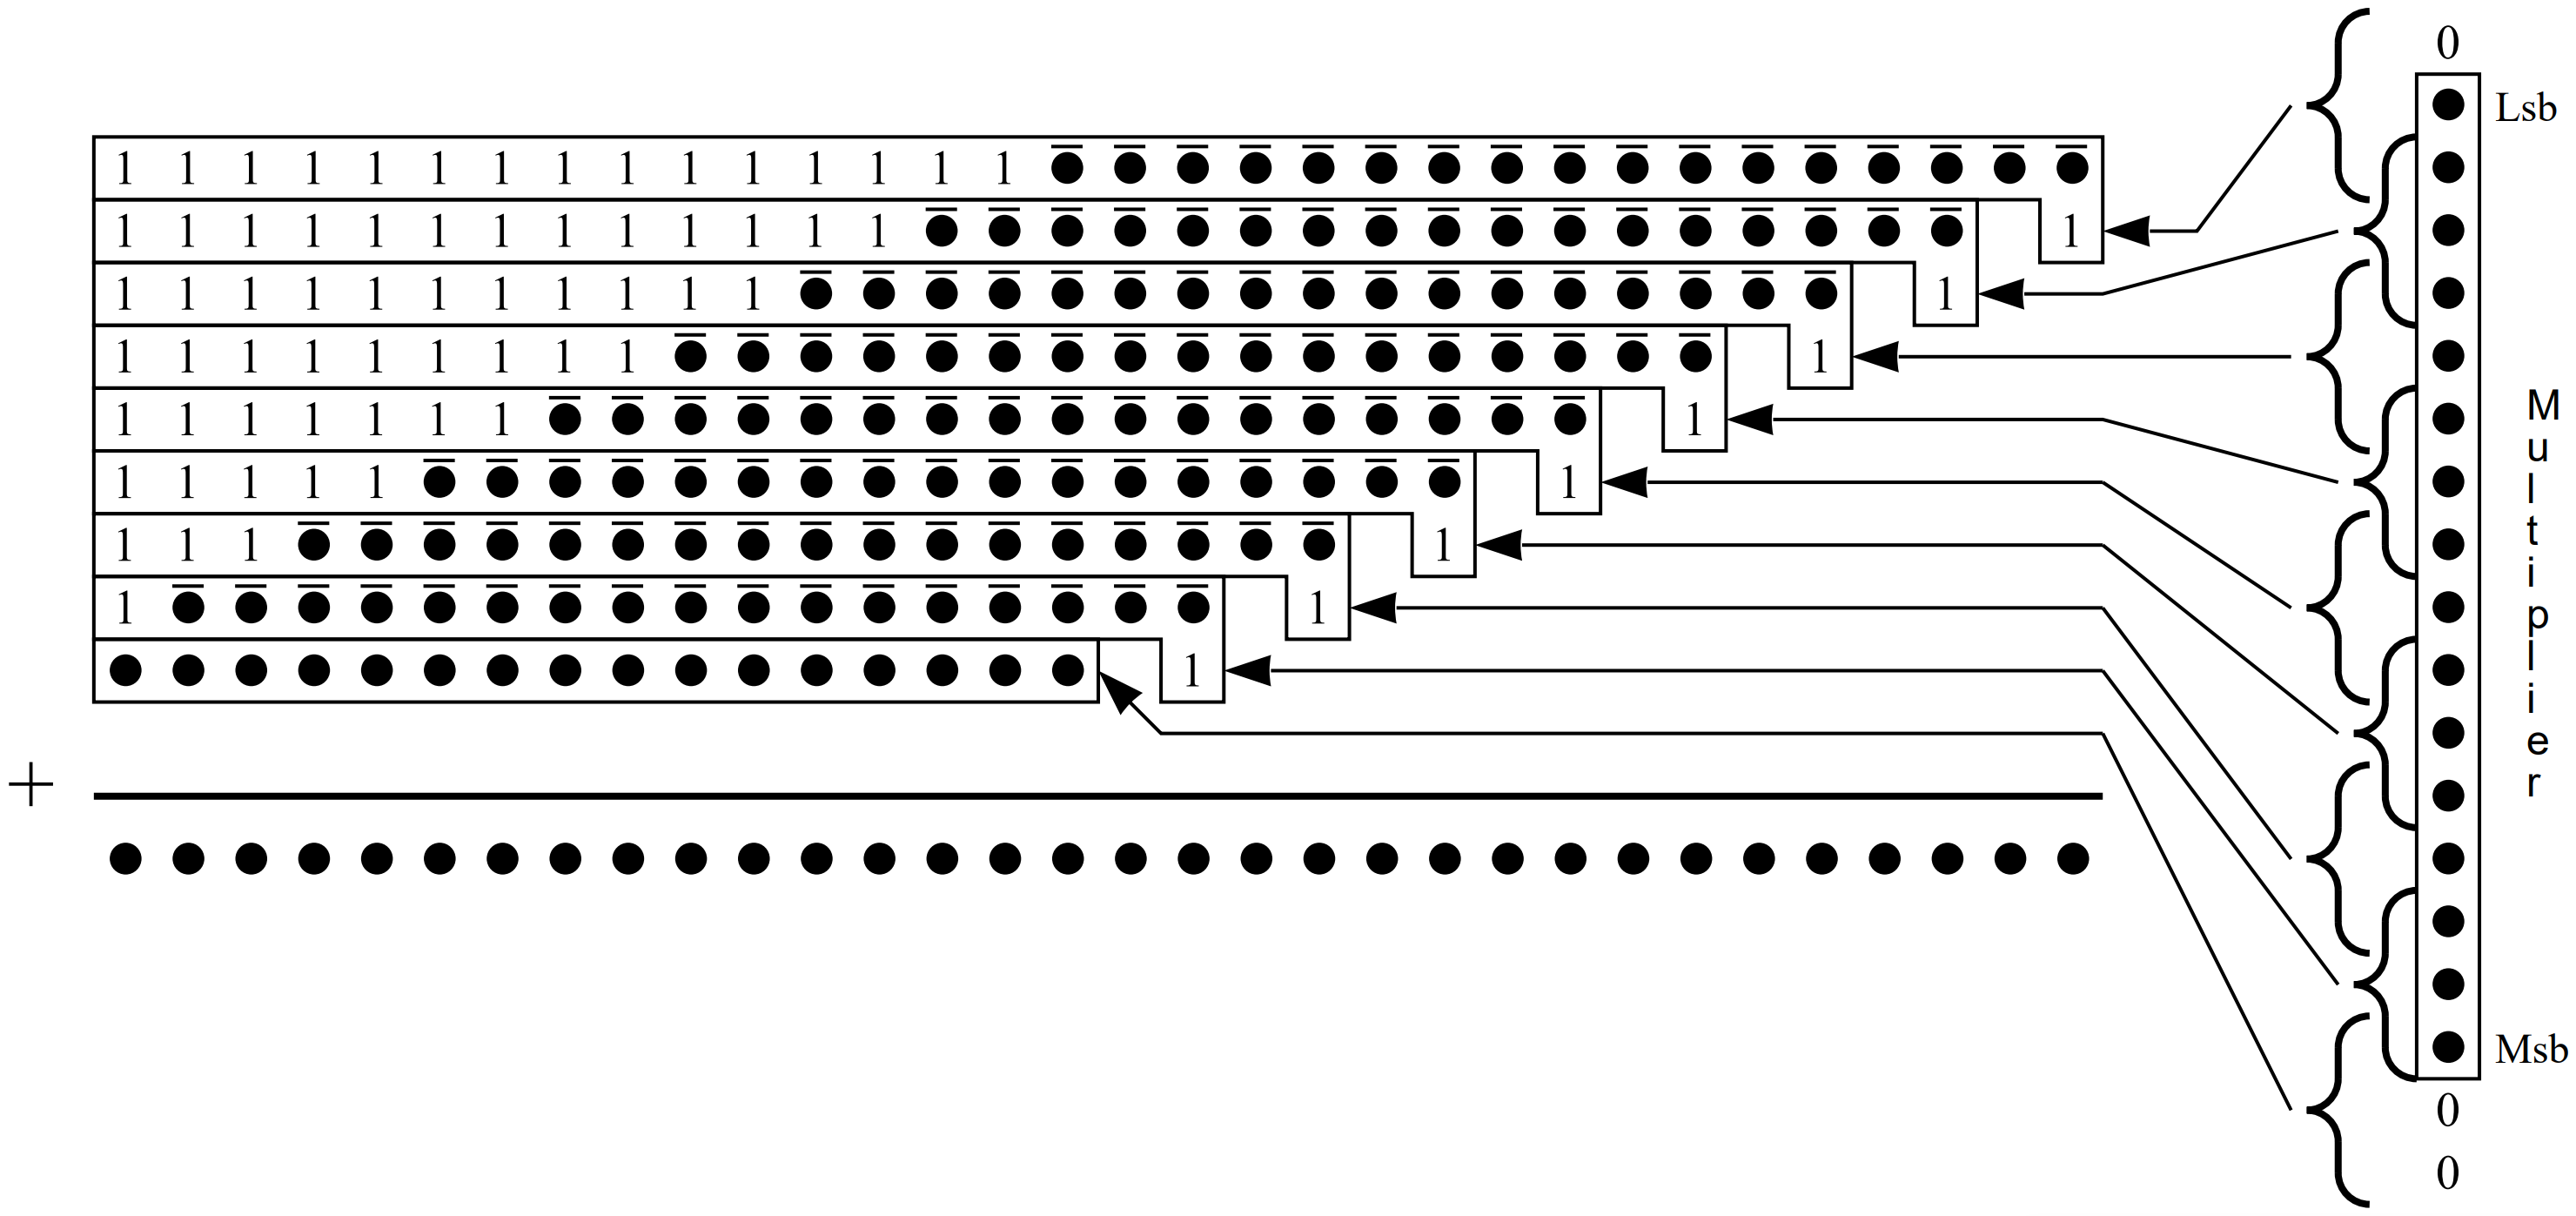
\includegraphics[width=\linewidth]{figs/EM-Fig-booth_unsign_negtive.png}
    \end{minipage}
    }
    \subfigure[部分积均为负数,高位进行1扩展后累加]{
    \label{EM:Fig:booth_16x16_unsign_PP_negtive_summed}
    \begin{minipage}[t]{0.48\linewidth}
    \centering
    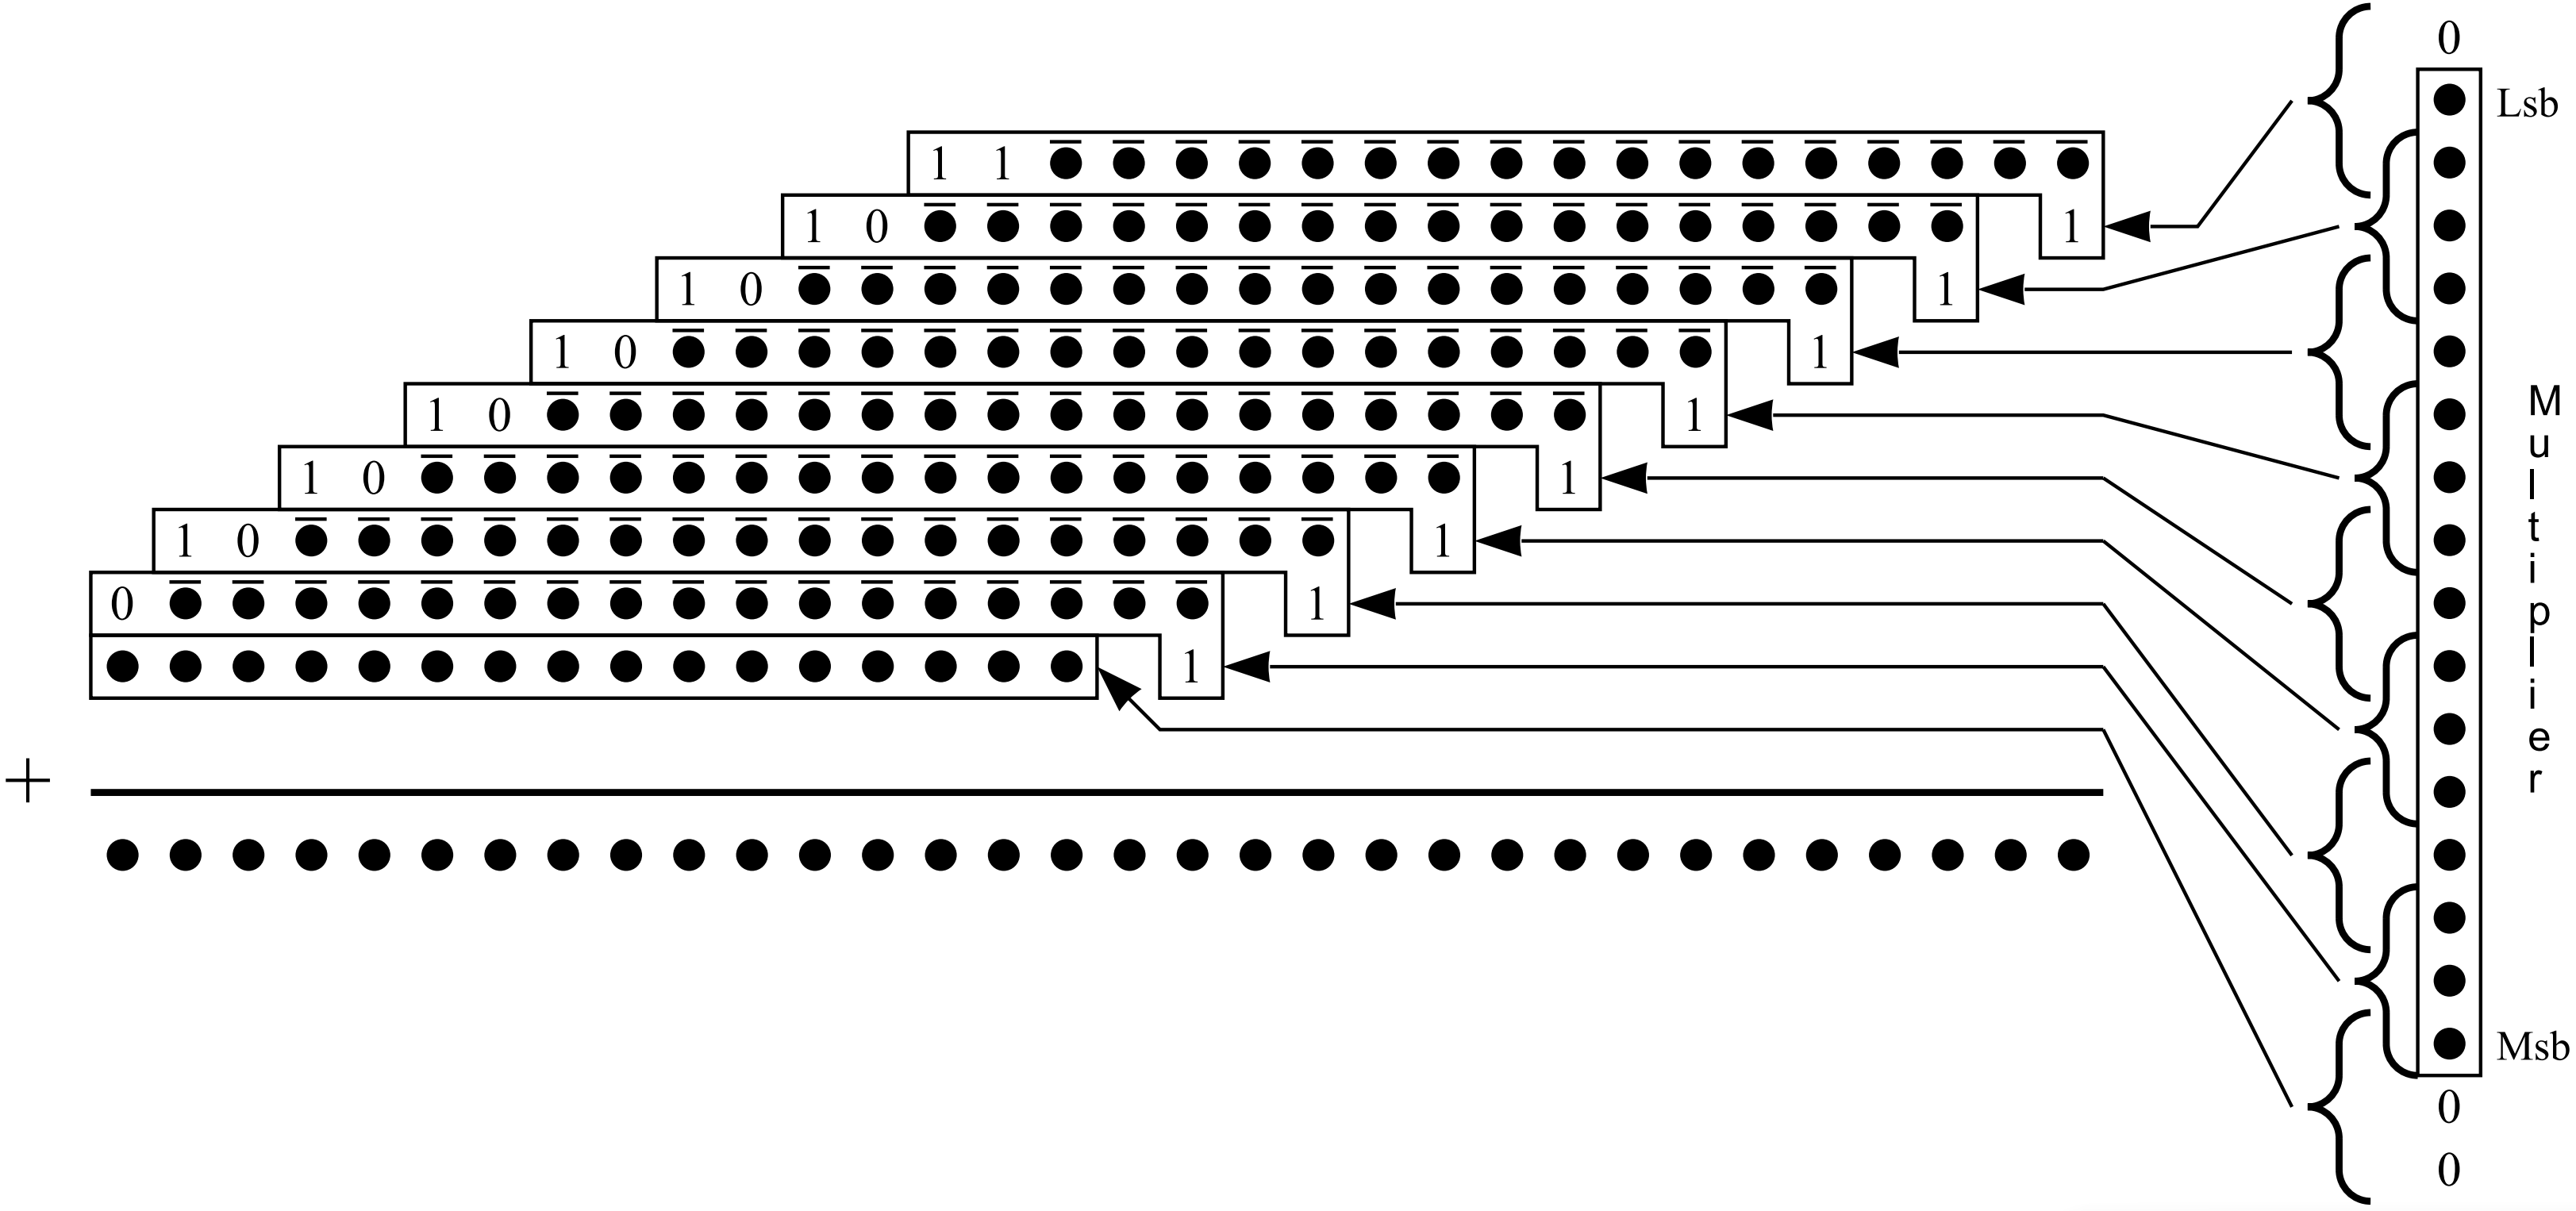
\includegraphics[width=\linewidth]{figs/EM-Fig-booth_unsign_negtive_summed.png}
    \end{minipage}
    }
    \subfigure[部分积正负均可的统一符号位扩展方法,$S$表示布斯码值的符号,$S=0$为正,$S=1$为负]{
    \label{EM:Fig:booth_16x16_unsign_PP_complete}
    \begin{minipage}[t]{0.48\linewidth}
    \centering
    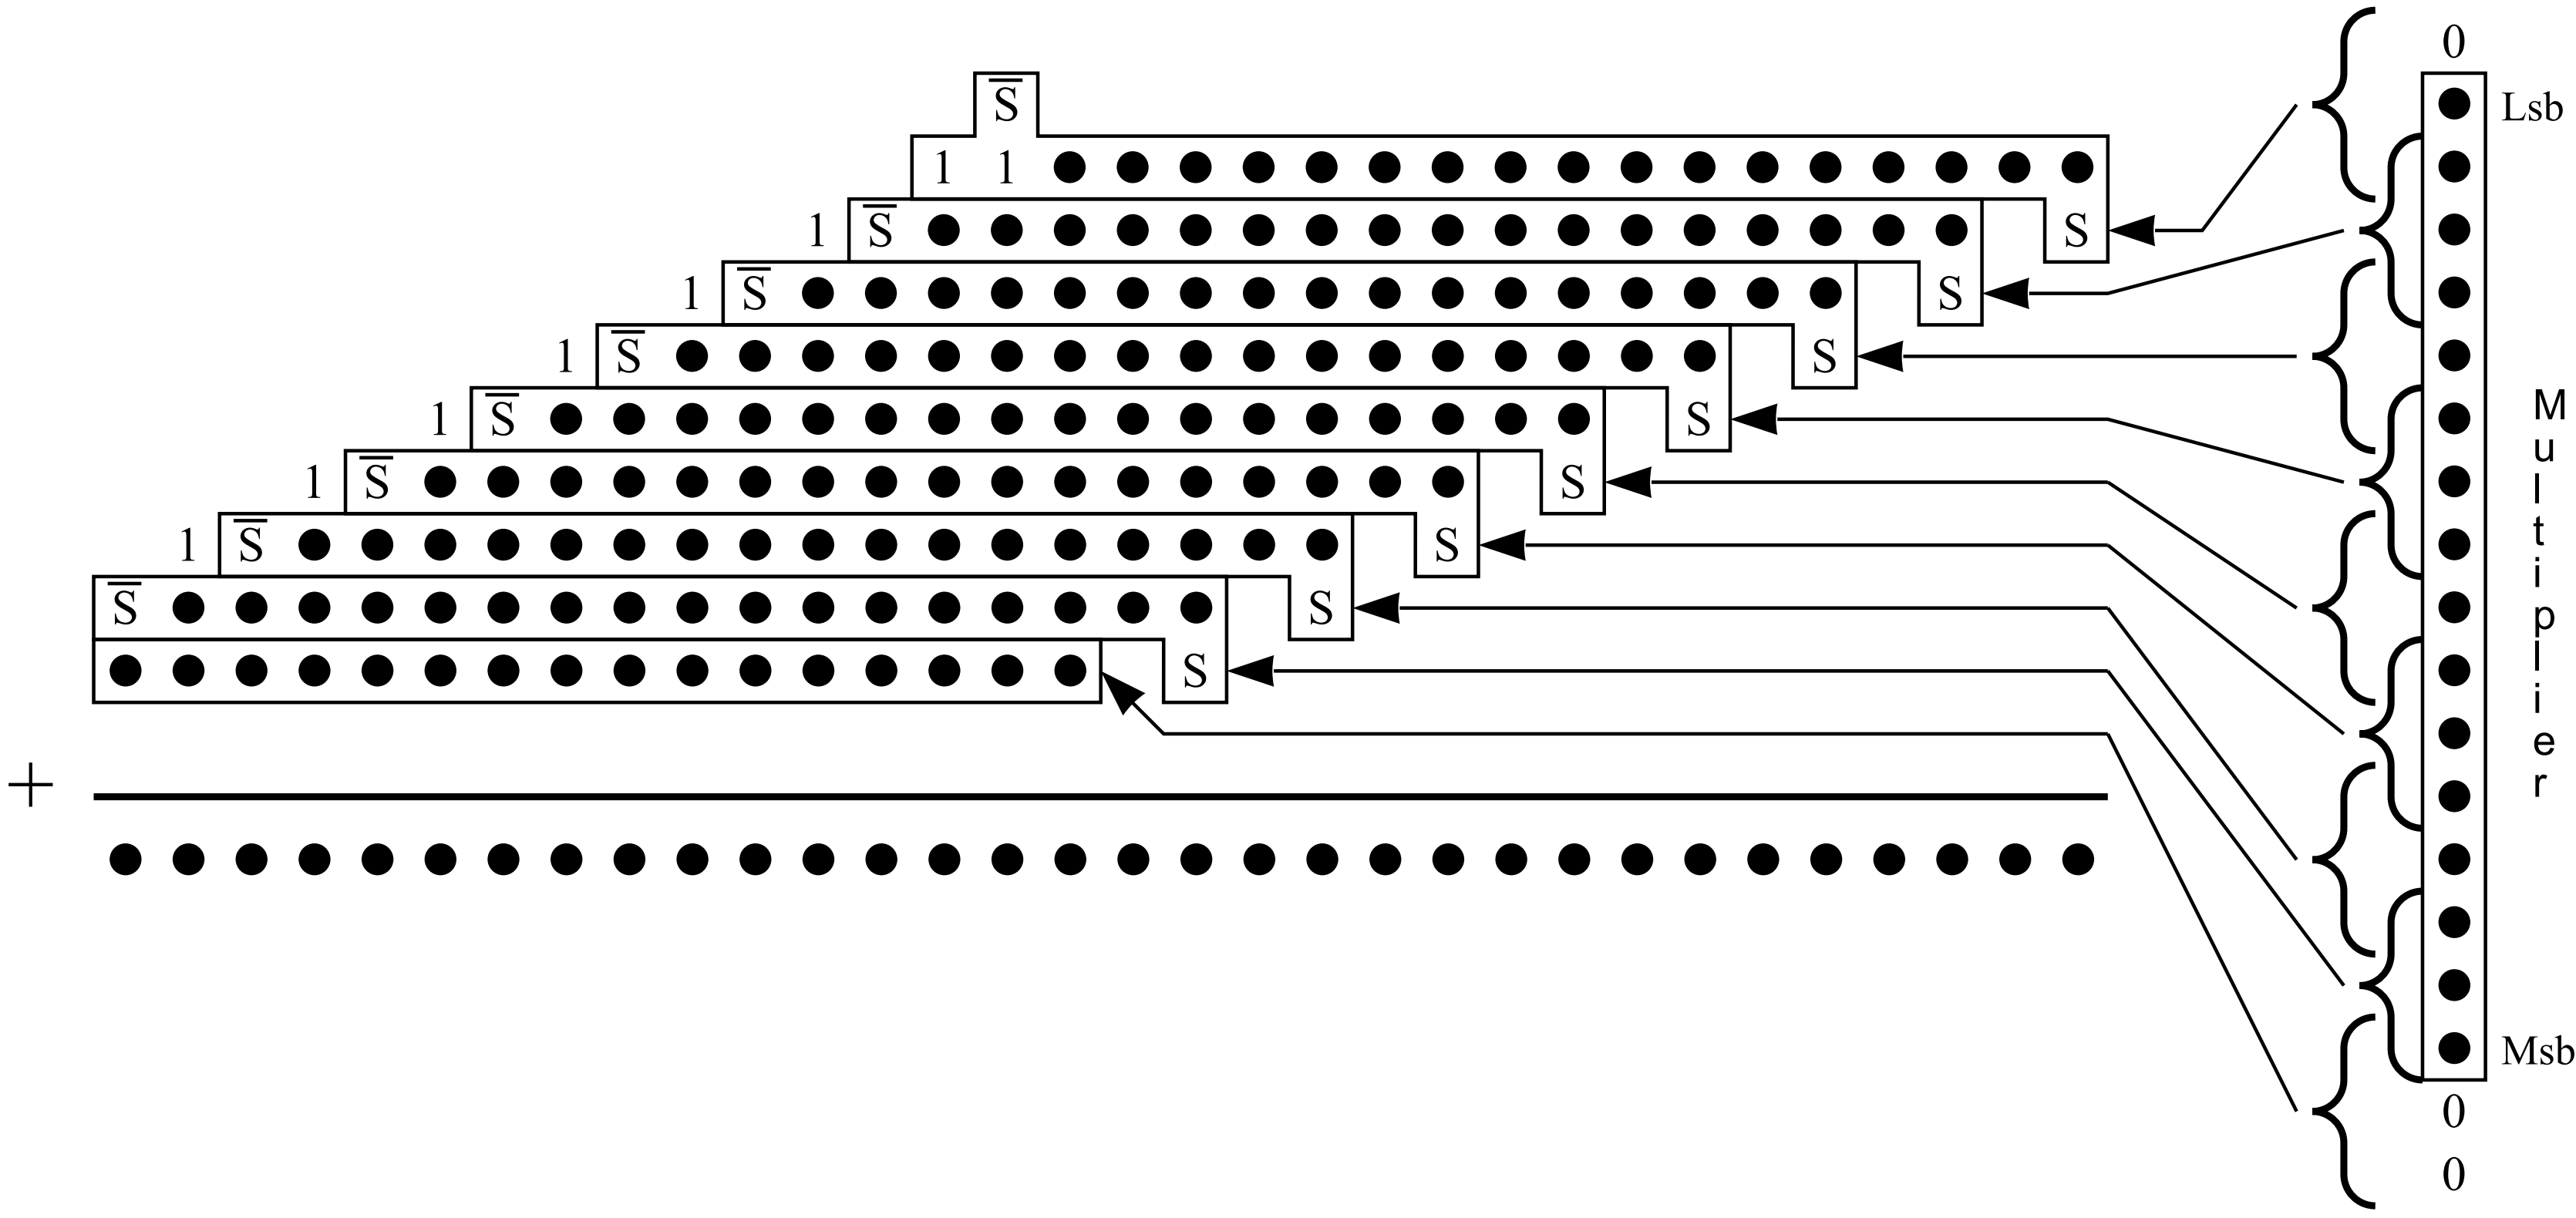
\includegraphics[width=\linewidth]{figs/EM-Fig-booth_unsign_complete.png}
    \end{minipage}
    }
    \subfigure[利用等价变换降低阵列层数后的部分积符号位扩展方法,$S$表示布斯码值的符号,$S=0$为正,$S=1$为负]{
    \label{EM:Fig:booth_16x16_unsign_PP_complete_reduce_height}
    \begin{minipage}[t]{0.48\linewidth}
    \centering
    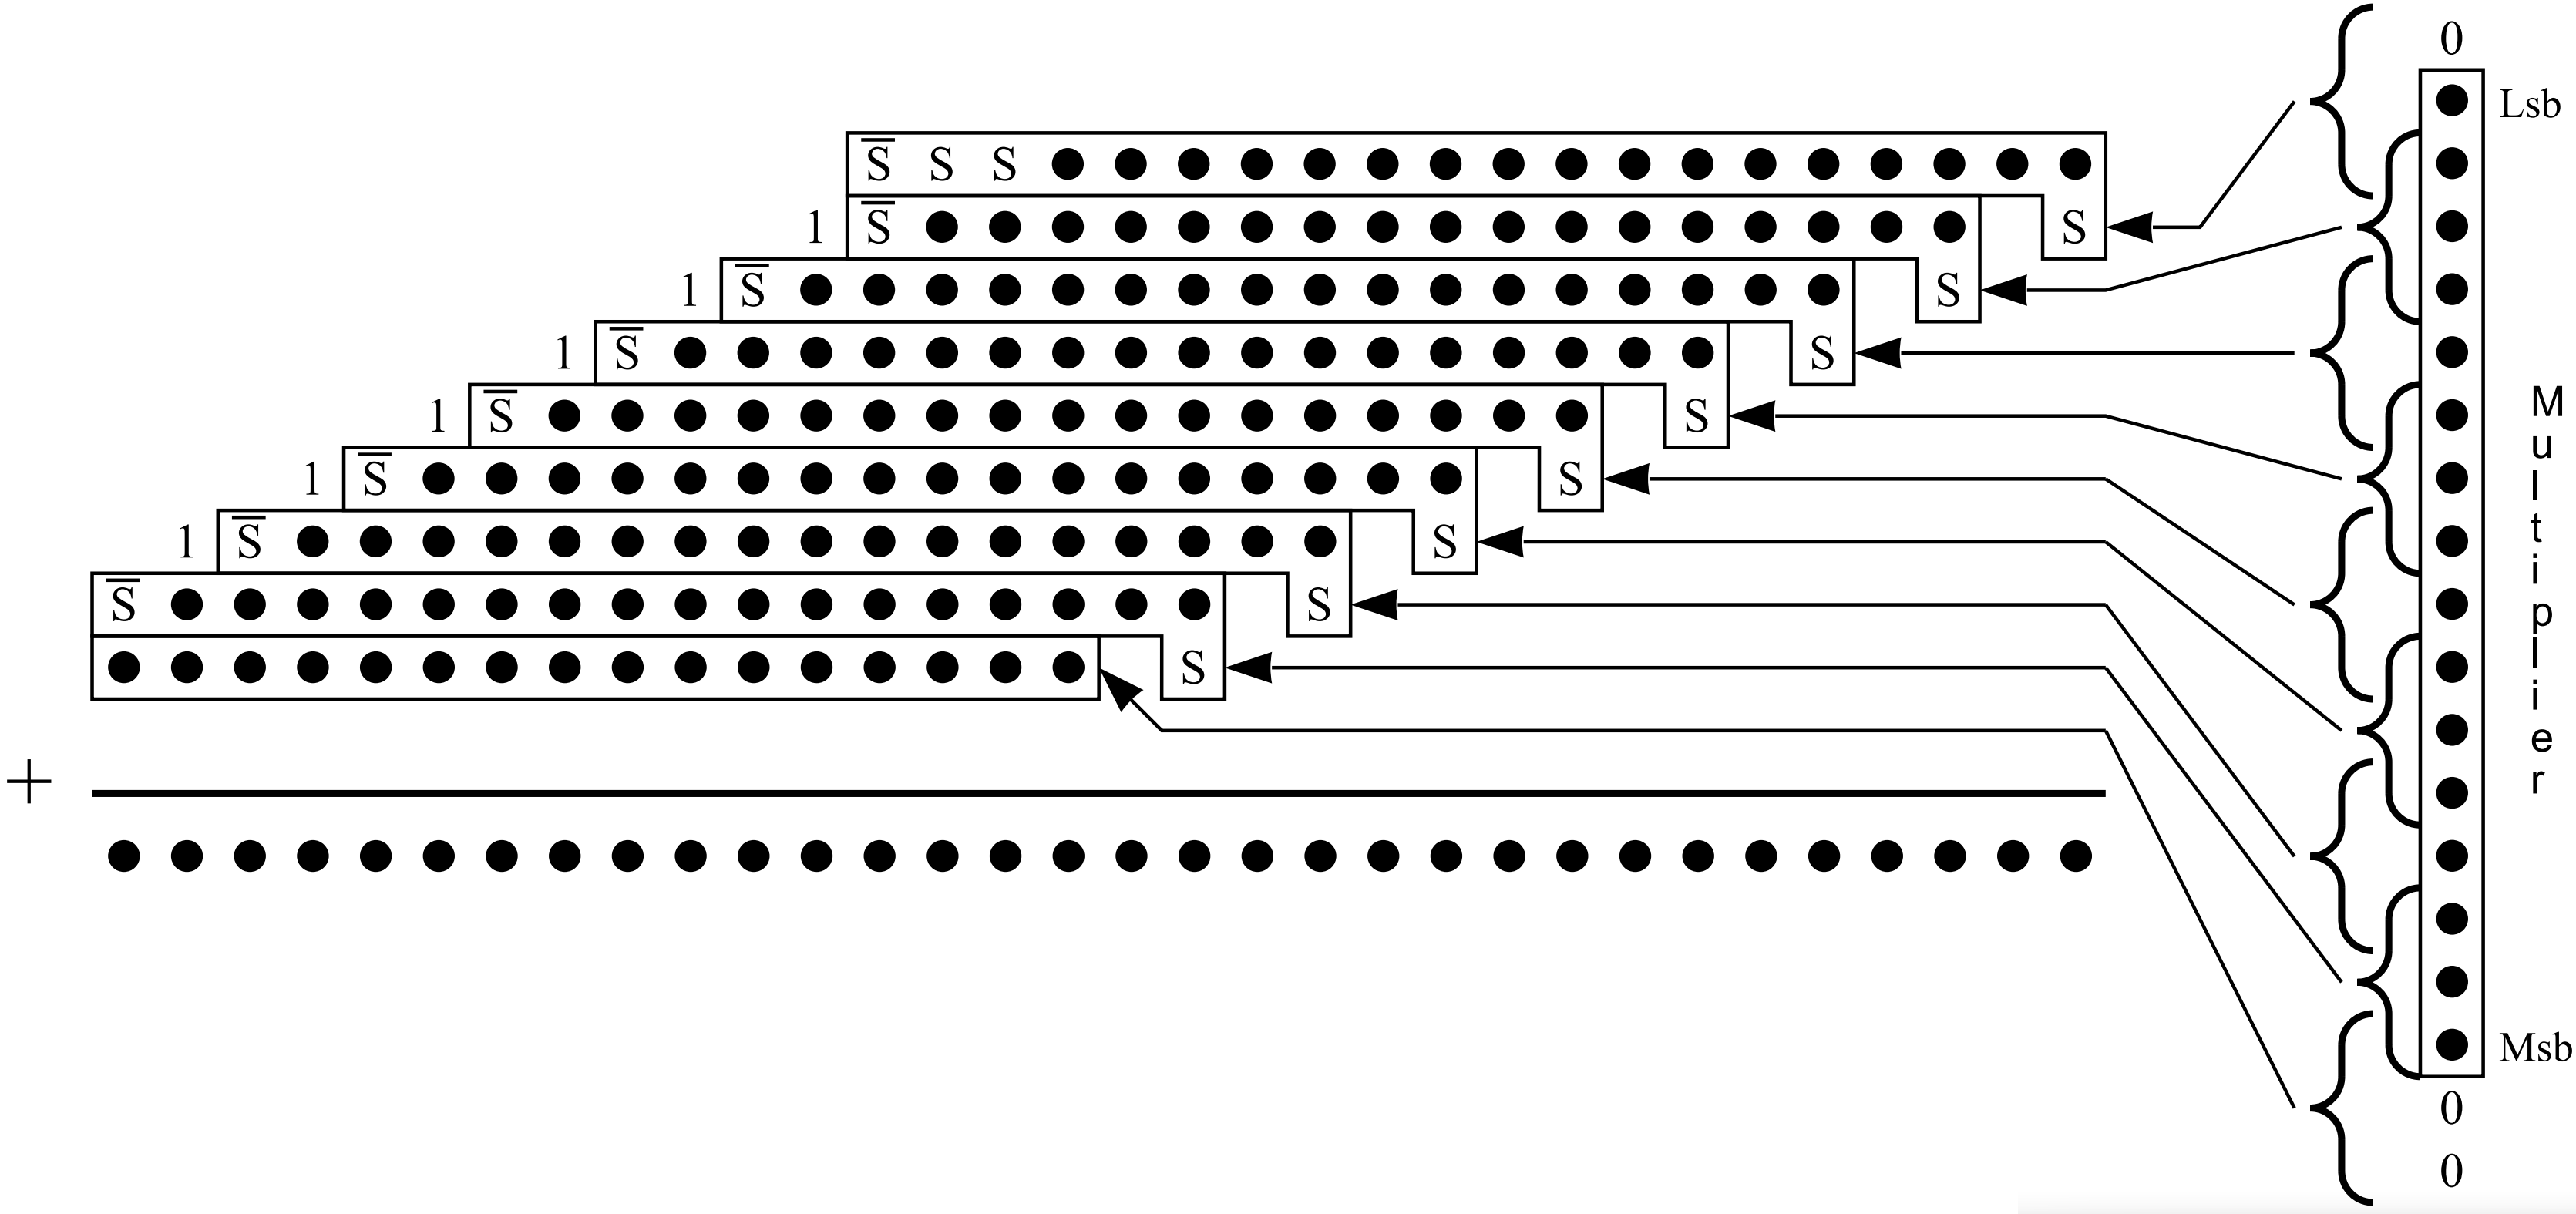
\includegraphics[width=\linewidth]{figs/EM-Fig-booth_unsign_complete_reduce_height.png}
    \end{minipage}
    }
\caption{$16\times16$无符号乘法的基4布斯算法部分积符号位扩展优化方法}
\label{EM:Fig:booth_16x16_unsign_PP}
\end{figure}

对于$16\times16$无符号数乘法,假设每个部分积是非负数,高位应进行0扩展,0可省略,省略后的部分积阵列如图\ref{EM:Fig:booth_16x16_unsign_PP_positive}所示,部分积总数为$8+1 = 9$个。除了最下面的那个部分积之外,每个部分积的位宽均为17比特。不考虑最下面那个部分积(该部分积永远是非负数),图\ref{EM:Fig:booth_16x16_unsign_PP_negtive}展示了所有部分积均为负数时的符号位扩展情况,即高位进行1扩展,在对扩展产生的左上角大量的1进行累加后的部分积阵列如图\ref{EM:Fig:booth_16x16_unsign_PP_negtive_summed}所示。
若图\ref{EM:Fig:booth_16x16_unsign_PP_negtive_summed}中存在部分积为正值,则需要对部分积的符号位进行修正,将高位的1扩展变回为0扩展,方法如图\ref{EM:Fig:booth_16x16_unsign_PP_complete}所示,引入$S$代表布斯码值的符号,$S=0$表示布斯码值为正,$S=1$表示布斯码值为负,达到对部分积进行统一符号位扩展的效果。最后,通过等价变换将\ref{EM:Fig:booth_16x16_unsign_PP_complete}中最上面的$\overline{S}$合并在部分积中,降低阵列的层数,如图\ref{EM:Fig:booth_16x16_unsign_PP_complete_reduce_height}所示,得到最终的常用的符号位扩展方法。

对布斯算法来讲,当乘数的位宽为偶数时,与同位宽的无符号乘法相比,补码有符号数乘法的部分积个数会少一个。另外,在符号位扩展方面的区别是,在假设部分积均为负数而实际可能为正数、将大量的1累加后、需要对部分积的符号位进行修正时,不能再单一的引入布斯码值的符号,而是要引入布斯码值符号$S$和被乘数符号的同或(Exclusive-NOR)进行修正。图\ref{EM:Fig:booth_16x16_signed_PP}展示了$16\times16$补码乘法的基4布斯算法部分积符号位扩展优化方法的示意图。
\begin{figure}[!htb]
    \centering
    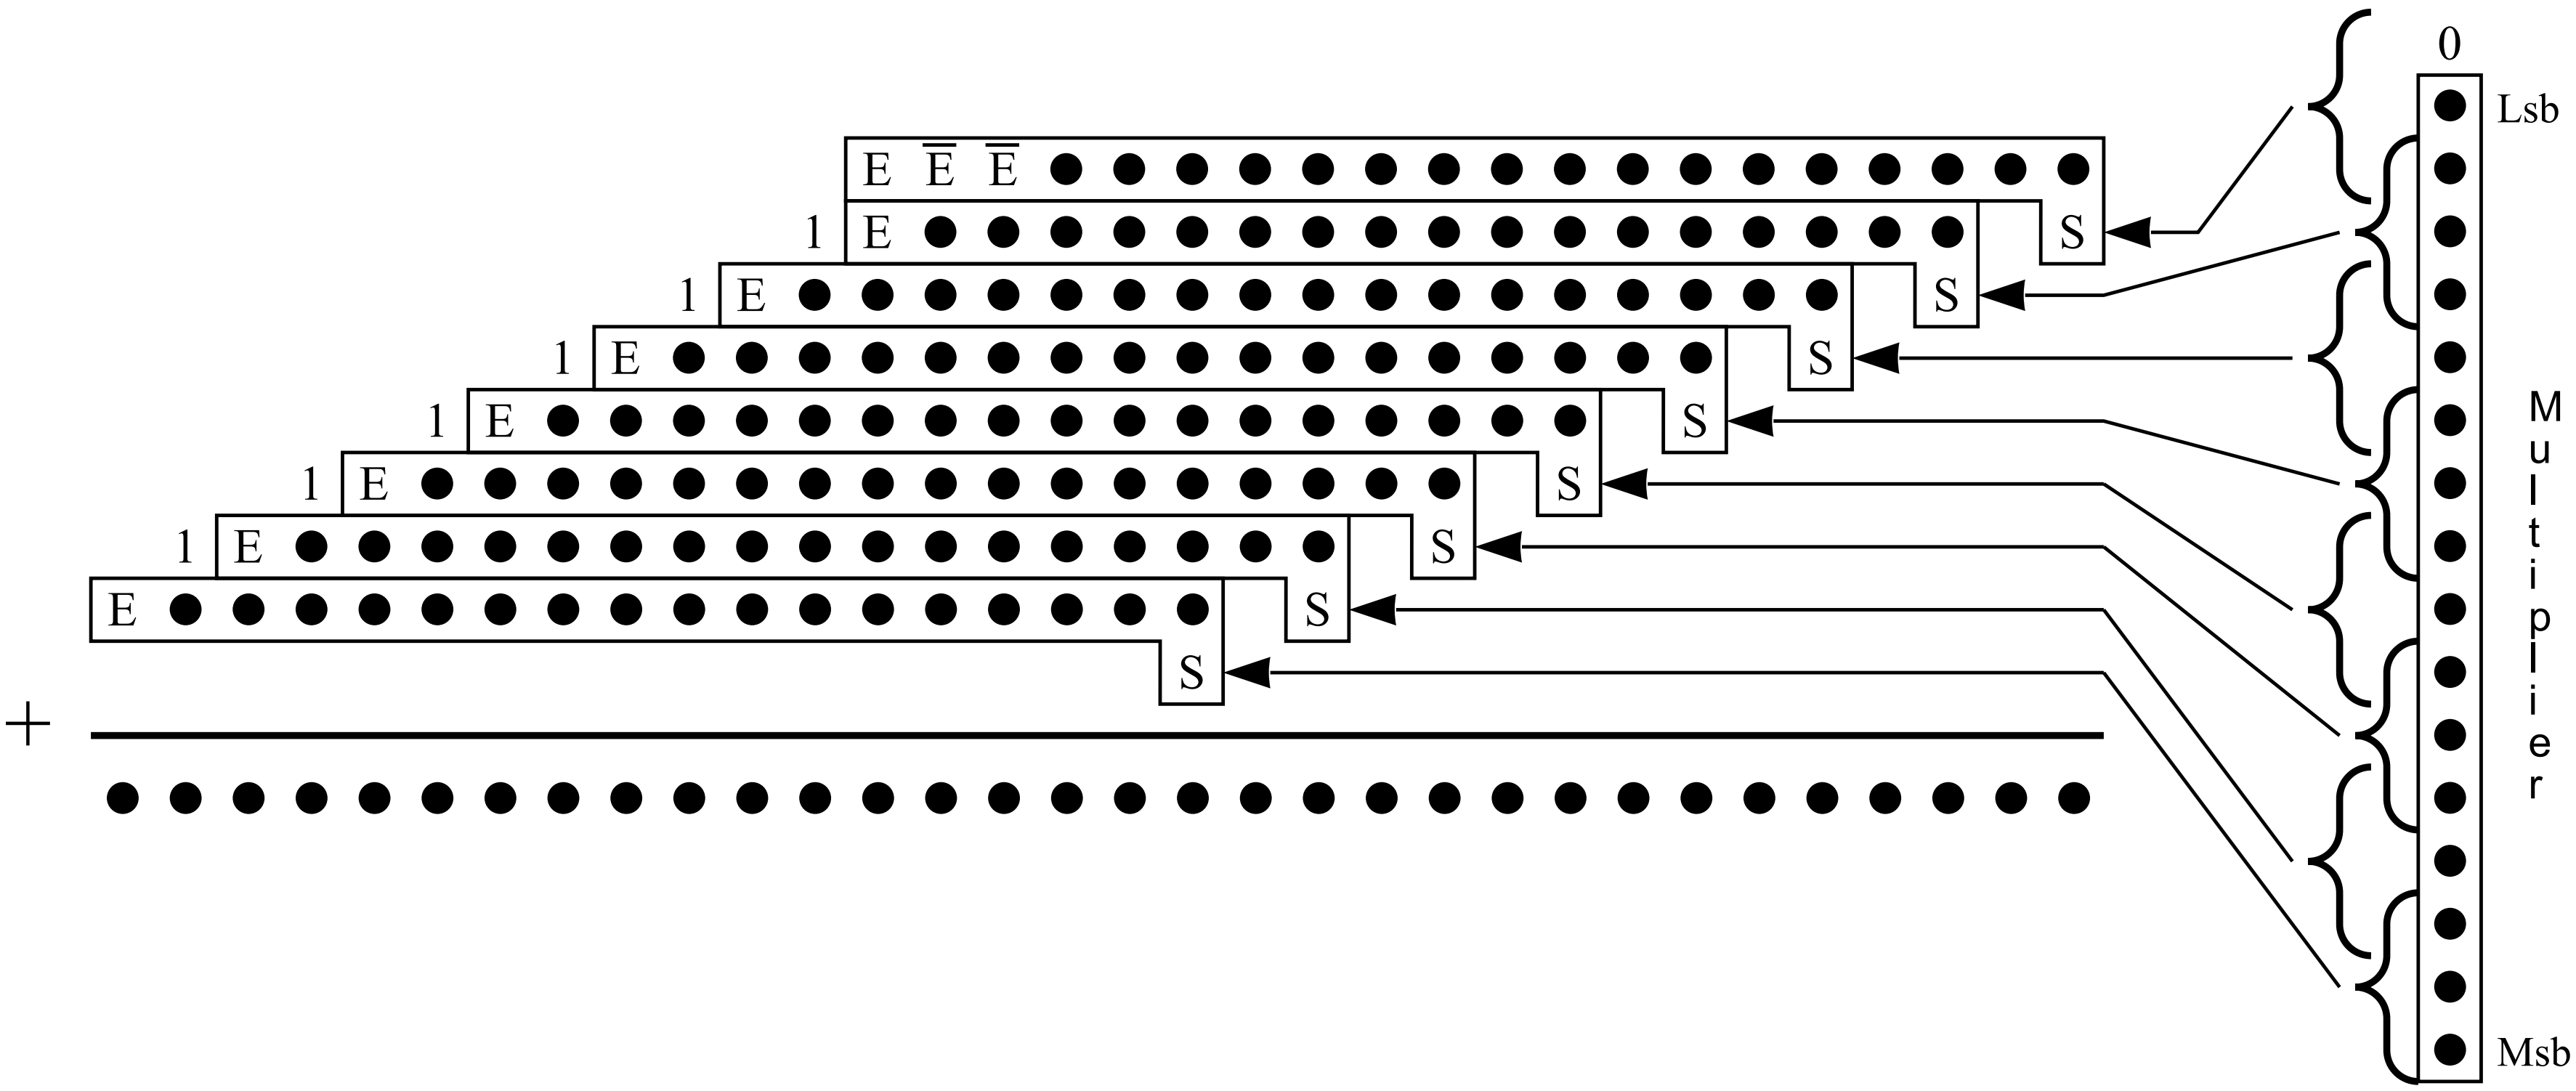
\includegraphics[width=\textwidth]{figs/EM-Fig-booth_signed.png}
    \caption{$16 \times 16$补码乘法的基4布斯算法部分积符号位扩展优化方法,$E$表示布斯码值符号$S$和被乘数符号的同或}
    \label{EM:Fig:booth_16x16_signed_PP}
\end{figure}

\subsection{部分积的累加}

部分积产生后需要进行累加,这种累加本质上是一种多操作数的加法。一个直接的累加方法是用许多全加器(Full Adder,FA)形成阵列,被称为阵列累加,更为先进的方法是以进位保留或树结构的形式完成的。

\subsubsection{阵列累加}

\begin{figure}[!htb]
    \centering
    \subfigure[$4\times4$无符号数乘法产生的部分积]{
    \label{EM:Fig:array_multiplier_unsigned}
    \begin{minipage}[t]{0.48\linewidth}
    \centering
    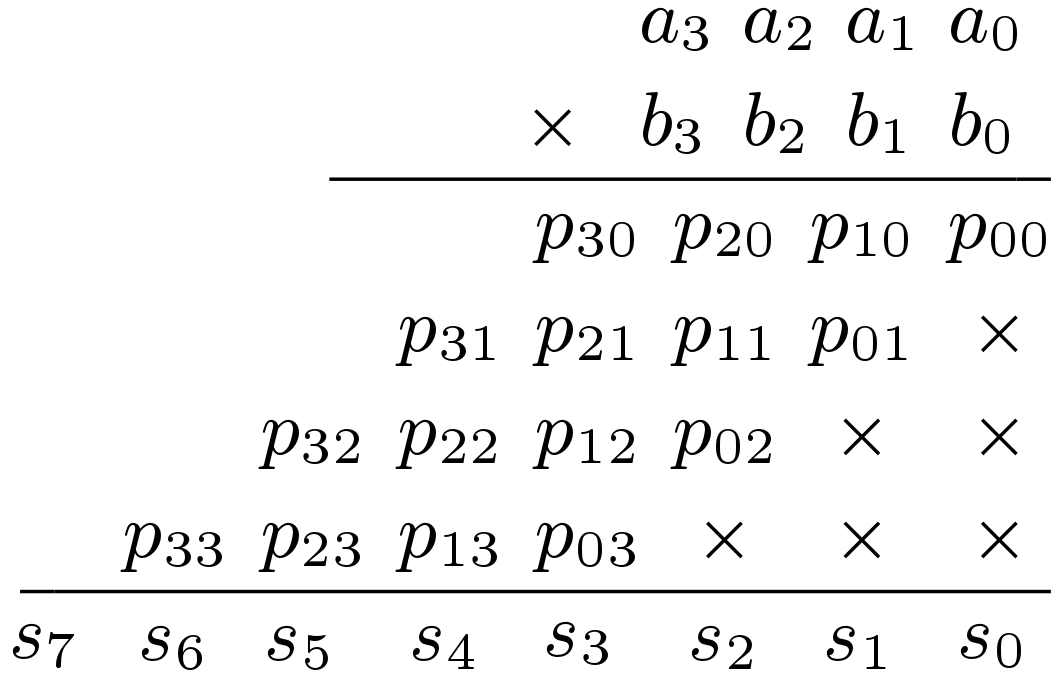
\includegraphics[width=\linewidth]{figs/EM-array_multiplier_unsigned.png}
    \end{minipage}
    }
    \subfigure[部分积的阵列累加电路]{
    \label{EM:Fig:array_multiplier_FA}
    \begin{minipage}[t]{0.48\linewidth}
    \centering
    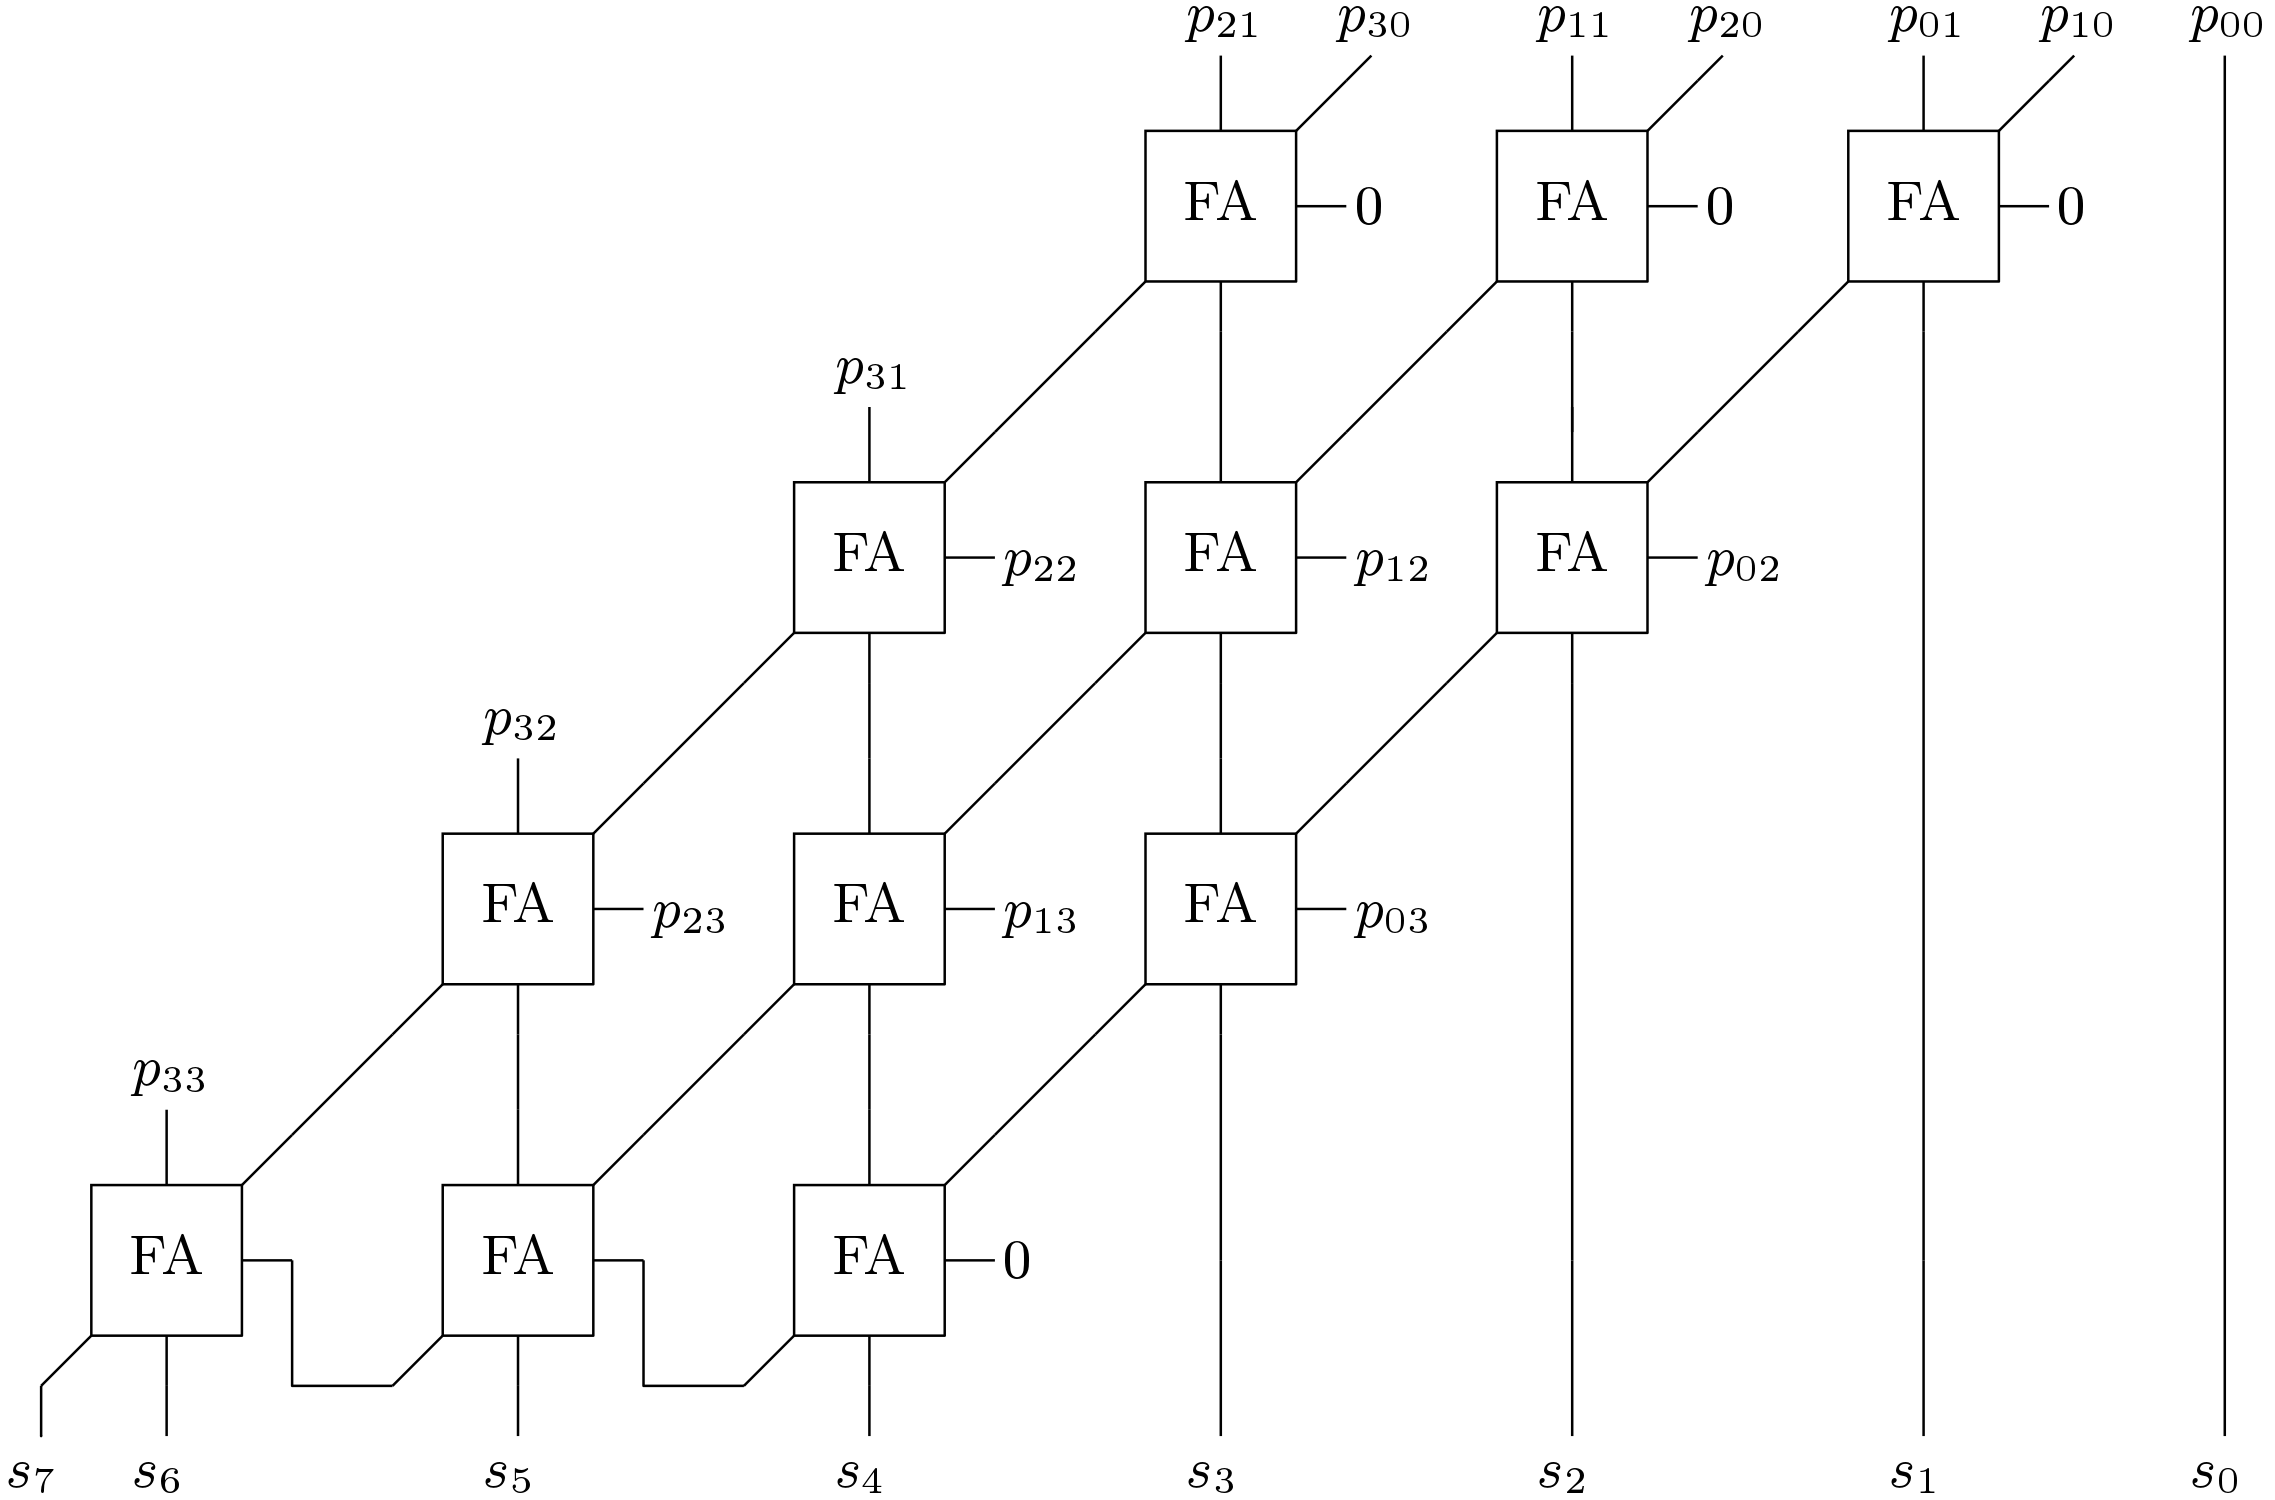
\includegraphics[width=\linewidth]{figs/EM-array_multiplier_FA.png}
    \end{minipage}
    }
\caption{$4\times4$无符号数乘法部分积及对应的阵列累加电路示意图}
\label{EM:Fig:array_multiplier}
\end{figure}

图\ref{EM:Fig:array_multiplier}展示了一个$4\times4$无符号数乘法部分积的生成及阵列累加电路示意图,部分积的移位操作通过布线即可完成,整个结构可以被很轻易的压缩成一个矩形,使得版图非常紧凑。阵列累加可以直接生成最终结果,并不需要最终相加这一步操作。然而,阵列结构中部分积的累加是通过逐位进位实现的,关键路径较长,性能较差。

\subsubsection{进位保留加法器}

进位保留加法器(Carry Save Adder,CSA)可以高效的对多个(通常是3个及以上)二进制数进行求和,通常用于乘法器中部分积的累加。在二进制中,两个或三个比特相加产生的进位不会超过1,基于这个发现,CSA的基本思想是通过全加器将进位信号和求和信号保存下来,不断累加,直到最后通过一个向量合并加法器得到最终结果。图\ref{EM:Fig:CSA}展示了一个4操作数8比特位宽,最后通过超前进位加法器进行向量合并的CSA结构图。
\begin{figure}[!htb]
    \centering
    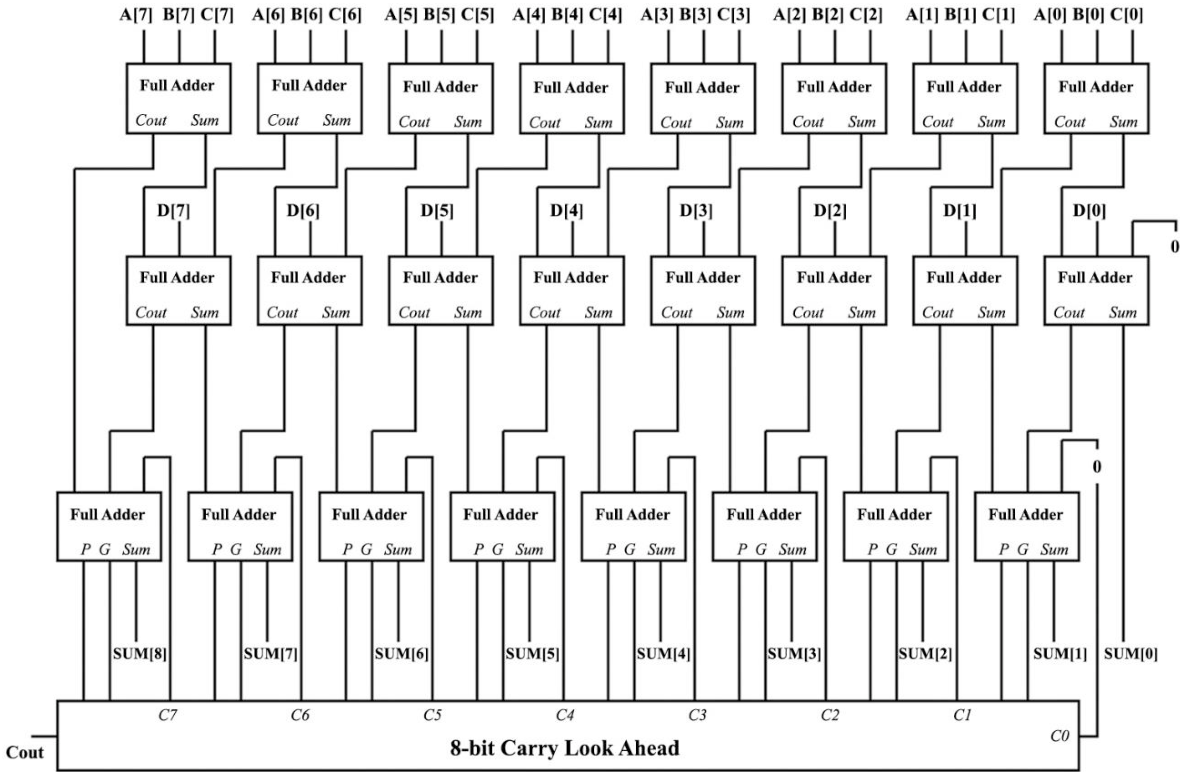
\includegraphics[width=0.85\textwidth]{figs/EM-CSA.png}
    \caption{4操作数8比特位宽,最后通过超前进位加法器相加的CSA结构图}
    \label{EM:Fig:CSA}
\end{figure}
从图中可以看到,4个8比特位宽的操作数经过两级全加器的压缩变成了2个操作数,其中第一级全加器产生了$A$、$B$和$C$的进位及求和,之后和$D$一起被第二级全加器进行压缩,最后送给向量合并加法器进行最终求和。与阵列累加的方式相比,CSA累加部分积的速度更快,性能更高。
注意这里的CSA并不会对操作数进行分组后并行累加,而是逐级累加\cite{数字集成电路_第十一章_设计运算功能块},这点与接下来讲的树形加法器有本质区别\footnote{https://blog.csdn.net/qq\_26707507/article/details/106146612}。

\subsubsection{树形加法器}

不论是阵列累加还是CSA累加本质上都是通过排列全加器实现的,事实上,全加器也可以安排为树形,这样既能减少累加电路所需的全加器的数量,还能降低关键路径延迟。树形加法器的实现可以看作是并行的进位保留加法器,累加效率更高。常见的树形加法器包括华莱士树\cite{EM:Wallace}和达达树\cite{EM:Dadda}。

(1)华莱士树

华莱士树(Wallace tree)加法器\cite{EM:Wallace}是由澳大利亚计算机科学家克里斯·华莱士(Christopher Stewart Wallace)于1964年设计的,被广泛用于乘法器中部分积的高效快速累加。其基本步骤如下:(a)假设所有部分积都是同时生成的,第一步是将部分积每3个分为一组(不足3个保持),并将每组部分积的个数通过全加器和半加器压缩为2个;(b)重复对部分积进行分组并压缩,直到只剩下两个部分积;(c)相加最后两个部分积得到最终结果。
\begin{figure}[!htb]
    \centering
    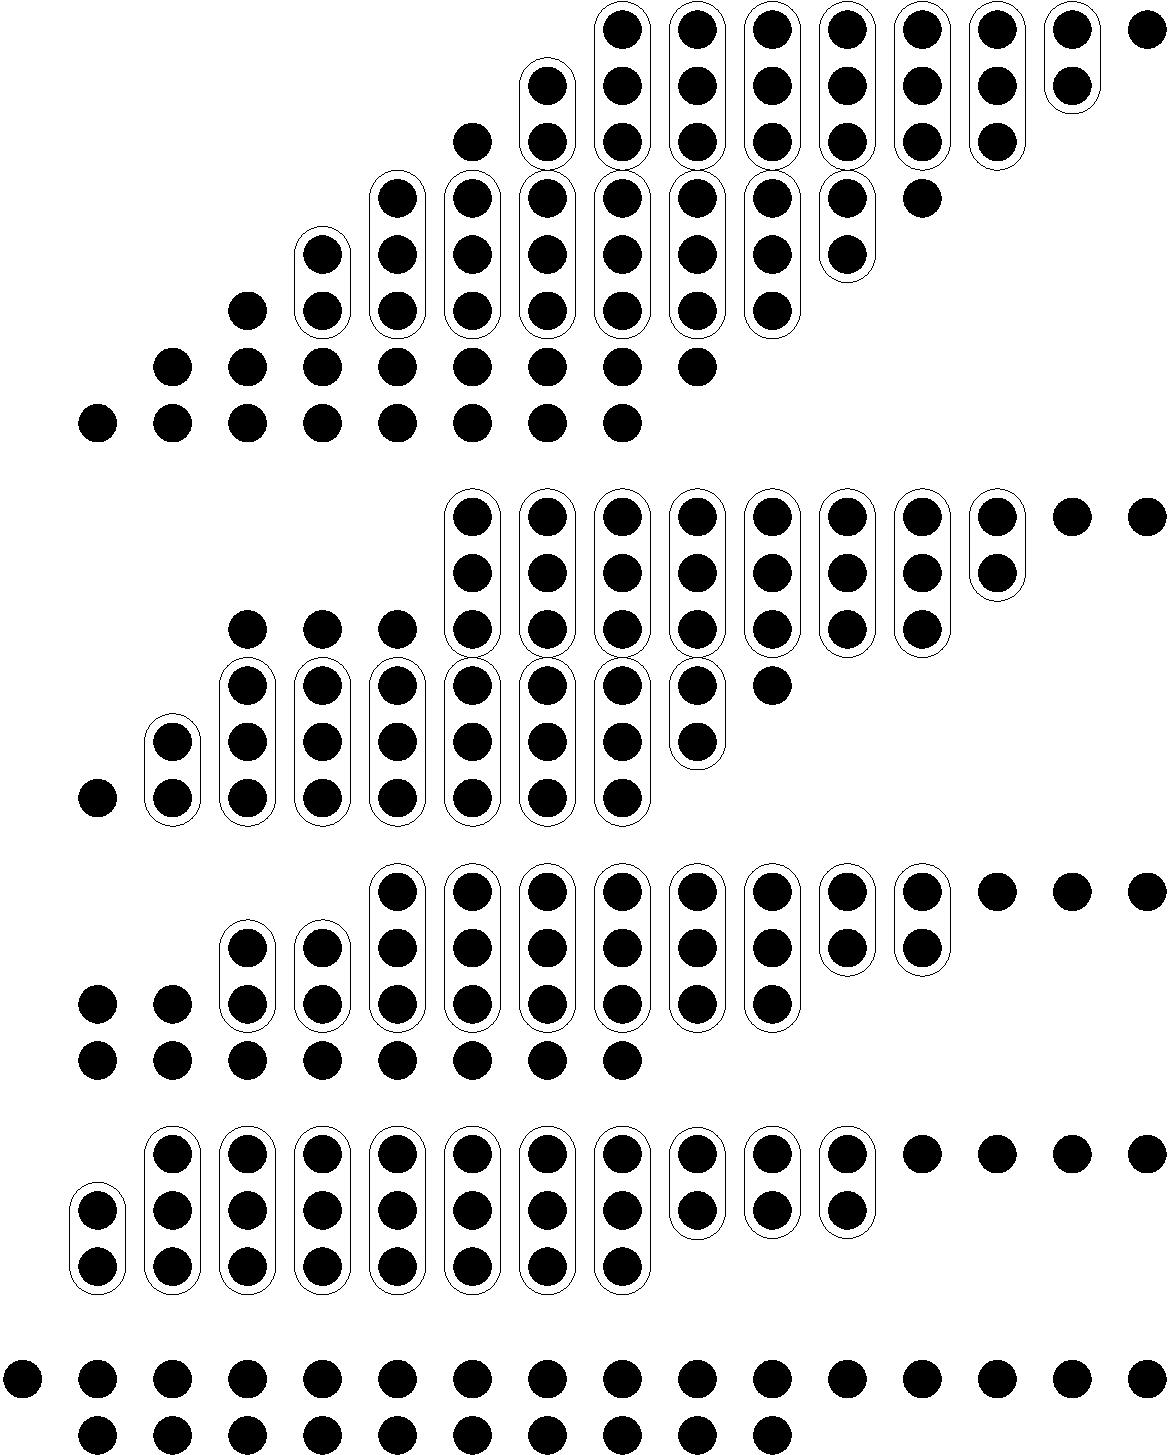
\includegraphics[width=0.85\textwidth]{figs/EM-wallace.pdf}
    \caption{利用华莱士树加法器对$8 \times 8$无符号数乘法部分积进行累加的示意图}
    \label{EM:Fig:wallace}
\end{figure}
图\ref{EM:Fig:wallace}展示了一个利用华莱士树加法器对$8 \times 8$无符号数相乘产生的部分积进行累加的过程示意图,每个点表示一个比特,每个圈代表一个全加器或半加器(包含两个点的圈代表半加器,包含三个点的圈代表全加器),一共分组并压缩了4次,消耗了15个半加器和38个全加器,将8个部分积变成了2个部分积。
与阵列累加方法和进位保留加法器相比,华莱士树加法器的速度很快,且位宽越大越明显,但它的缺点是电路结构非常不规则,难以获得高质量的版图设计。改进的华莱士树方法能够使用更少的半加器,降低设计的复杂度\cite{EM:redeuce_wallace}。全加器本质上是一个3:2压缩器,能够将乘法器中每组部分积的数目减少至三分之二。在进一步地设计4:2甚至更高比例的压缩器之后,结合华莱士树方法可以得到性能更高的乘法器\cite{EM:wallace_42}。

(2)达达树

达达树(Dadda tree)加法器是由计算机科学家Luigi Dadda于1965年发明的一种树形加法结构\cite{EM:Dadda},与华莱树方法类似,达达树也是采用全加器和半加器对部分积进行压缩,直到最后只剩下两个部分积。与华莱士树相比,达达树使用了数量最少的全加器以及半加器重构了树,且树的级数(深度)不变,在节省了硬件资源的情况下保证了相似的速度。但是,达达树产生的最后两个部分积的位宽可能会稍大。具体步骤如下\footnote{https://en.wikipedia.org/wiki/Dadda\_multiplier}:
\begin{itemize}
    \item 部分积的累加过程由一个正整数序列$d_j$来控制:$d_1=2$,$d_{j+1}=\lfloor 1.5 \rfloor d_j$,$\lfloor \ \rfloor$表示向下取整;
    \item 初始的$j$应尽可能大并满足$d_j < n$,$n$是乘数的位宽(部分积阵列的高度);
    \item $j$逐步递减,且任意$j$下对部分积阵列从最低权重列开始遍历:(a)若列高度小于或等于$d_j$,跳过;(b)若列高度等于$d_j+1$,运用半加器在该列最上面的两个比特,产生进位及求和;(c)若列高度大于$d_j+1$,运用全加器在该列最上面的三个比特,产生进位及求和,并对该列重复(a)、(b)和(c)操作。注意列的高度可能需要考虑到前一列的进位;
    \item 累加结束时$j=1$,$d_j=2$(部分积只有两行),之后使用一个向量合并加法器求得最终结果。
\end{itemize}

图\ref{EM:Fig:dadda}展示了一个运用达达树对$8 \times 8$无符号数乘法生成的部分积进行压缩的过程示意图,该树的深度与图\ref{EM:Fig:wallace}中的华莱士树的深度相同,但使用了更少的全加器和半加器:达达树使用了35个全加器、7个半加器,华莱士树使用了38个全加器、15个半加器。
\begin{figure}[!htb]
    \centering
    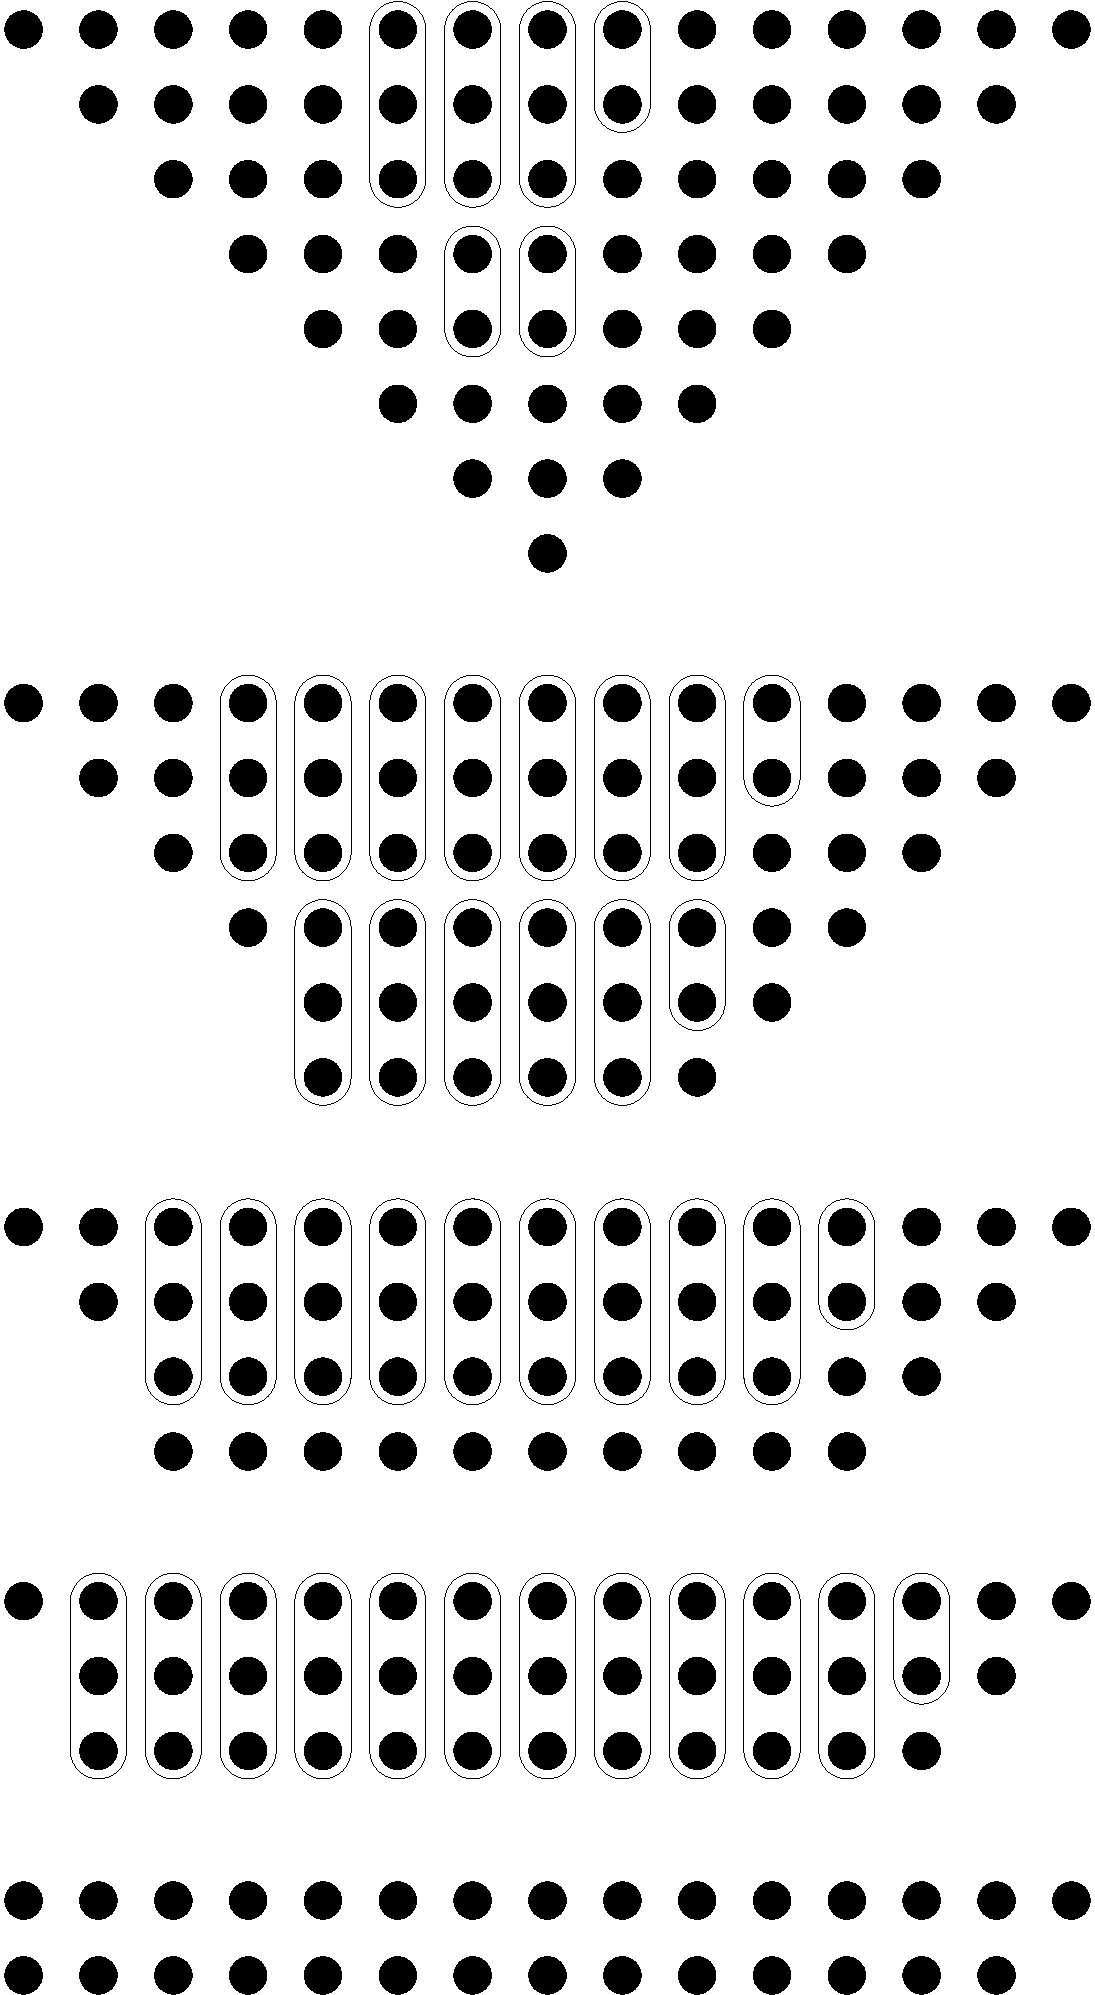
\includegraphics[width=0.7\textwidth]{figs/EM-dadda.pdf}
    \caption{利用达达树加法器对$8 \times 8$无符号数乘法部分积进行累加的示意图}
    \label{EM:Fig:dadda}
\end{figure}

\subsection{最终相加}

除了阵列累加方式以外,进位保存加法器、树形加法器等高速的部分积求和电路通常在最后都需要一个向量合并加法器(Vector-Merging Adder,VMA)进行最终两个部分积的相加,目前常见的VMA有以下几种结构:

\subsubsection{行波进位加法器}

行波进位加法器(Ripple-Carry Adder,RCA)又被称为逐级进位加法器,是由一系列全加器级联而成,优点是面积小、占用资源少,缺点是速度慢、效率低。在最好情况下,任何位宽的RCA都不需要传递进位信号也可以得到正确结果;但在最坏情况下,得到最终结果的延迟会随着位宽的增加而线性增大,从而限制了系统的运算速度。

\subsubsection{超前进位加法器}

当加法器的位宽较大时,由于RCA在最坏情况下每一级全加器的计算必须等待前一级的进位输出,导致其关键路径较长,效率较低。超前进位加法器(Carry-Lookahead Adder)的思想是并行计算每一级全加器的进位输出,本质上是数学公式推导的结果,原理如下:

假设RCA中第$i$级全加器的输入为$a_i$、$b_i$、$c_{i}$,进位输出为$c_{i+1}$,设$p_i = a_i \oplus b_i$,$g_i = a_i b_i$,有:
\begin{equation}
\begin{aligned}
    c_{i+1} = & \ a_i b_i + c_i(a_i \oplus b_i) \\
    = & \ g_i + c_i p_i
\end{aligned}
\label{EM:Eq:CLA}
\end{equation}
若$p_i=1$,则$g_i =0$,$c_{i+1}=c_i$;若$p_i=0$,则$c_{i+1}=g_i$。因此$p_i$和$g_i$分别被称为第$i$级加法进位的传播信号和生成信号。
对$c_{i}, c_{i-2},c_{i-3},\cdots,c_{1}$使用式\eqref{EM:Eq:CLA},可将对$c_{i+1}$的求解转换为输入数的逻辑与(AND)和逻辑异或(XOR)操作(假设$c_0=0$),避免了RCA中的进位依赖问题,实现了效率的提升。与RCA相比,CLA的关键路径短,速度快,进位链计算依赖少。但在加法器位宽较大时,CLA中高位的进位输出表达式涉及的变量较多,存在较大扇入扇出的问题;同时,组合逻辑电路的输入信号过多也会引起竞争冒险(Race hazard),产生毛刺(Glitch),影响系统的稳定性。所以在加法器位宽较大时,要想利用CLA提高进位效率,需要先对操作数进行划分,对每个部分实行CLA,CLA块间再通过级联或嵌套等方式进行连接\footnote{https://zhuanlan.zhihu.com/p/378267920},以避免大输入位宽逻辑门的产生。其中,采用级联对各CLA块进行连接的方式被称为分块CLA,采用嵌套对各CLA块进行连接的方式被称为分级CLA。
灵活地对操作数进行划分并嵌套,能够得到许多不同的CLA结构,可在面积和速度之间进行权衡,存在一套能够简洁表示各种分级超前进位结构的符号体系,这一点会在后面的并行前缀加法器中详细讲述。
最后需要注意的是,基于CLA方法实现的加法器的面积和复杂度通常会比同等位宽的RCA大。

\subsubsection{进位旁路加法器}

对\eqref{EM:Eq:CLA}来说,一个$n$位RCA的最坏情况发生在$p_{n-1}, p_{n-2}, \cdots, p_0$均为1的时候(即$p_{n-1} p_{n-2} \cdots p_0=1$),注意此时$g_{n-1}, g_{n-2}, \cdots, g_0$均为0,式\eqref{EM:Eq:CLA}变为:
\begin{equation}
    c_{i+1} =  c_i
\label{EM:Eq:CSKA_prop}
\end{equation}
进位旁路加法器(Carry-Skip Adder,为了与进位保存加法器区分,这里缩写为CSKA,也叫Carry-bypass adder)的思想便是加速该情况下进位链的传播。一个$n$位的CSKA包括一个$n$位的RCA、一个$n$位的多输入与门(AND)、以及一个二选一的多路选择器(Multiplexer,MUX),图\ref{EM:Fig:CSKA_4bit}展示了一个4比特CSKA的结构图,$p_0 \sim p_3$信号通过与门连接到MUX上作为选择信号,当$p_0 p_1 p_2 p_3=1$时,$c_0$通过MUX直接输出,中间的RCA被旁路掉,大大减少了延迟。
\begin{figure}[!htb]
    \centering
    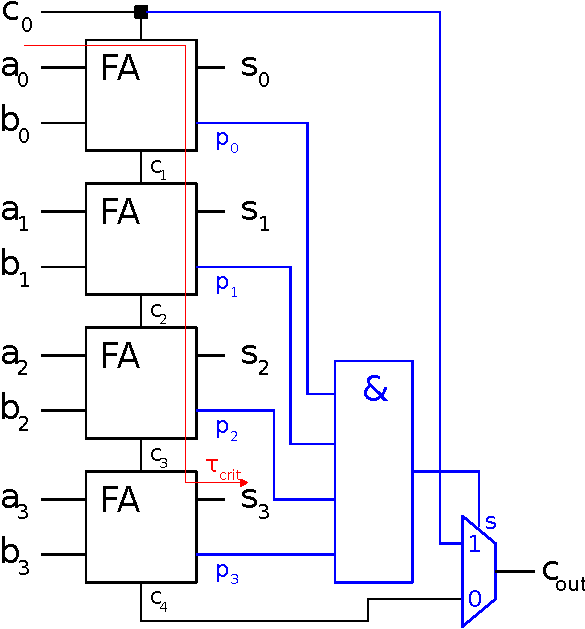
\includegraphics[width=0.4\textwidth]{figs/EM-CSKA_4Bit.pdf}
    \caption{一个4比特CSKA的结构示意图,FA代表全加器}
\label{EM:Fig:CSKA_4bit}
\end{figure}
但是,与RCA相比,CSKA并没有明显的性能改进(如图\ref{EM:Fig:CSKA_4bit}中的关键路径$\tau_{\text{crit}}$同样需要经过4个全加器),当位宽较大时,通过分块CSKA(Block CSKA,BCSKA)的方法可取得较为显著的速度增益。若一个$n$比特的分块CSKA有$m$块CSKA,每块CSKA的位宽均为$\dfrac{n}{m}$,则该分块CSKA被称为固定大小分块CSKA\footnote{https://en.wikipedia.org/wiki/Carry-skip\_adder}。
\begin{figure}[!htb]
    \centering
    \includegraphics[width=\textwidth]{figs/EM-CSKA_16Bit.pdf}
    \caption{一个固定大小分块CSKA的例子:通过级联4个4比特CSKA实现16比特加法}
\label{EM:Fig:CSKA_16bit}
\end{figure}

图\ref{EM:Fig:CSKA_16bit}展示了一个通过级联4个4比特CSKA实现16比特加法的固定大小分块CSKA的结构图,其关键路径(红色线条$\text{T}_{\text{critical}}$)延迟包括头尾两个4比特RCA的延迟和中间两个旁路逻辑中MUX的延迟。从静态时序分析(Static Timing Analysis, STA)的角度看,图\ref{EM:Fig:CSKA_16bit}的关键路径延迟比一个16比特的RCA更差,但STA得到的关键路径是伪路径,电路实际运行过程中并不会发生。固定大小分块CSKA真实的关键路径可通过以下过程来理解:输入同时到来后,每块CSKA很快地被确定为是否处于旁路状态;之后所有的CSKA同时计算,假设首块CSKA没有被旁路,当首块CSKA的进位输出得到后,后面所有的CSKA要么处于旁路状态、要么也已计算完毕。
因此固定大小分块CSKA的最坏情况是,进位信号需要通过首尾两个RCA和中间全部处于旁路状态的CSKA中的MUX。通过调整块的大小和层级,分块CSKA的性能可得到进一步的优化。
最后需要注意的是,与其他快速加法器如CLA不同,分块CSKA的性能仅在输入是某些情况下会获得提高,即速度的提高是概率性的。

\subsubsection{进位选择加法器}

另一种避免出现RCA中最坏情况下逐级进位的方法是预先考虑进位输入的两种可能的值(0和1),并提前计算针对这两种可能性的结果,一旦进位输入的值确定,正确的结果可以通过一个简单的MUX选出,这一设想的实现被称为进位选择加法器(Carry-Select Adder,为了与进位保存加法器区分,这里缩写为CSEA)。CSEA通常只包括RCA和MUX,一个4比特位宽的CSEA的结构如图\ref{EM:Fig:CSEA_basic}所示,由于一个RCA的进位为0,而另一个RCA的进位为1,因此可通过实际进位输入决定哪个RCA的结果作为输出。与同等位宽的RCA相比,除了MUX以外,CSEA消耗了两倍数量的全加器,是面积换性能的典型代表。
\begin{figure}[!htb]
    \centering
    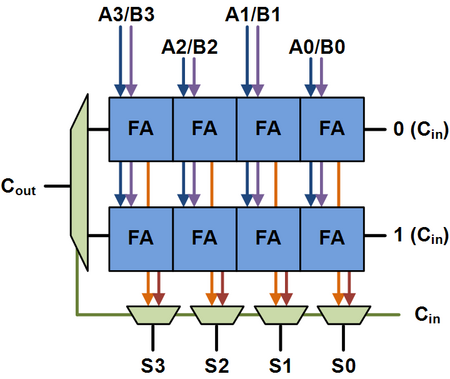
\includegraphics[width=0.5\textwidth]{figs/EM-CSEA_basic.png}
    \caption{一个4比特CSEA的结构图,FA代表全加器}
\label{EM:Fig:CSEA_basic}
\end{figure}

完整的CSEA加法器需要对多个小的CSEA进行级联,并额外引入一个RCA。若每个小CSEA的位宽相同,该加法器被称为线性(Linear)CSEA;若每个小CSEA的位宽不同,该加法器被称为可变大小(Variable-sized)CSEA,一种特殊的可变大小CSEA是平方根(Square-root) CSEA。

(1)线性进位选择加法器

\begin{figure}[!htb]
    \centering
    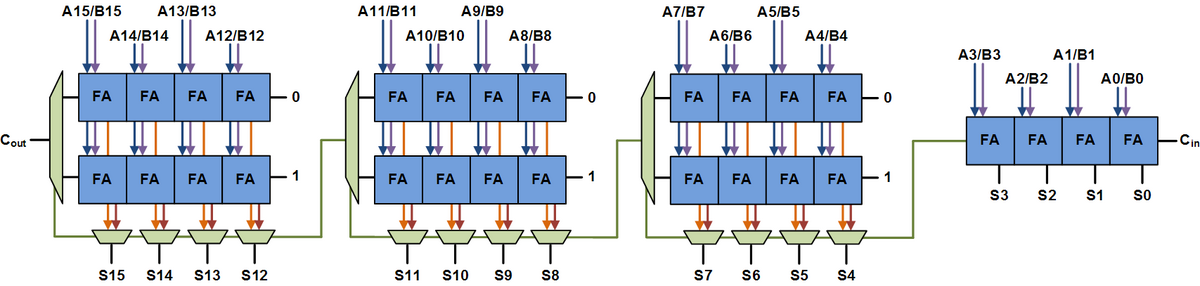
\includegraphics[width=\textwidth]{figs/EM-CSEA_linear.png}
    \caption{一个16比特线性进位选择加法器示意图}
\label{EM:Fig:CSEA_linear}
\end{figure}

图\ref{EM:Fig:CSEA_linear}展示了一个16比特线性CSEA的结构示意图,该加法器由一个4比特RCA和三个4比特CSEA组成,其关键路径包括初始的4比特RCA和后续三个MUX,可通过以下过程理解:当初始的RCA计算完成时,后面所有的小CSEA中的RCA也均计算完成,只需等待真正的进位输入信号进行选择即可。
通常来讲,对于一个$n$比特线性CSEA,每个小CSEA的位宽取$\lfloor \sqrt n \rfloor$性能最好\footnote{https://en.wikipedia.org/wiki/Carry-select\_adder},这里$\lfloor \ \rfloor$代表向下取整。

(2)平方根进位选择加法器

若级联的每个小CSEA的位宽不同,且数值大小从低位到高位依次为$2$、$3$、$4$、$\cdots$,初始RCA的位宽为2,则该可变大小CSEA被称为平方根CSEA,如图\ref{EM:Fig:CSEA_square}所示,关键路径为初始的2位宽的RCA和后续的3个MUX。
\begin{figure}[!htb]
    \centering
    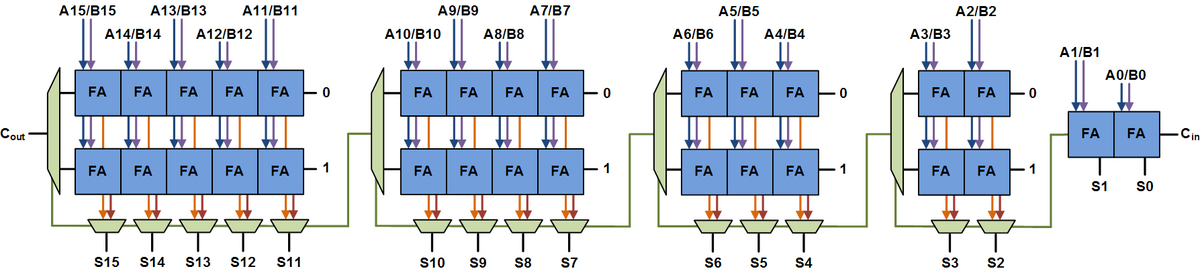
\includegraphics[width=\textwidth]{figs/EM-CSEA_square.png}
    \caption{16比特平方根进位选择加法器示意图}
\label{EM:Fig:CSEA_square}
\end{figure}
平方根CSEA假设全加器和MUX的延迟相等,避免了线性CSEA中高位CSEA计算完成后等待进位输入信号选择的缺点,不论位宽多大,其关键路径总是初始的2位宽RCA加上后续的MUX,与线性CSEA相比取得了显著的性能提升。不过,一般情况下全加器和MUX的延迟不相等,因此需要根据实际情况决定使用哪种结构的CSEA。

\subsubsection{并行前缀加法器\cite{EM:book_Computer_Arithmetic}}

由式\eqref{EM:Eq:CLA}可得:
\begin{align}
    c_{i+1} = & \ \textcolor{blue}{g_i} +\textcolor{blue}{p_i} c_i \notag \\
          = & \ g_i + p_i \textcolor{red}{(g_{i-1} + p_{i-1} c_{i-1})} \notag \\
          = & \ \textcolor{blue}{(g_i + p_i g_{i-1})} + \textcolor{blue}{(p_i p_{i-1})} c_{i-1} \notag \\
          = & \ (g_i + p_i g_{i-1}) + (p_i p_{i-1}) \textcolor{red}{(g_{i-2} + p_{i-2} c_{i-2})} \notag \\
          = & \ \textcolor{blue}{(g_i + p_i g_{i-1} + p_i p_{i-1} g_{i-2})} + \textcolor{blue}{(p_i p_{i-1} p_{i-2})} c_{i-2} \notag \\
          = & \ \cdots
\label{EM:Eq:PPA_CLA}
\end{align}
可以看到,若将$p$和$g$的定义从单比特拓展到连续的多比特,设$i$、$j$均是整数且$0 \le i < j$,有:
\begin{align}
    & g_{[i,j]} =  g_j + p_j g_{j-1} + p_j p_{j-1} g_{j-2} + \cdots + (p_j p_{j-1} p_{j-2} \cdots p_{i+1}) g_i \notag \\
    & p_{[i,j]} = p_j p_{j-1} p_{j-2} \cdots p_i \notag \\
    & c_{j+1} = g_{[i,j]} + p_{[i,j]} c_i
\label{PPA_multi_bit_gp}
\end{align}
即对加法块$[i,j]$来讲同样存在进位的生成信号$g_{[i,j]}$和传播信号$p_{[i,j]}$,考虑到两者总是成对出现,可将其简写为二元对$(g_{[i,j]},p_{[i,j]})$。对两个相邻、部分重叠或完全重叠的加法块,$(g_{[i,j]},p_{[i,j]})$有如下性质:

相邻:假设$k$是整数且$i<k<j$,则块$[i,k-1]$与块$[k,j]$相邻:
\begin{align}
    g_{[i,j]} = & \ g_{[k,j]} + g_{[i,k-1]} p_{[k,j]} \notag \\
    p_{[i,j]} = & \ p_{[i,k-1]} p_{[k,j]}
\label{EM:Eq:PPA_相邻}
\end{align}

部分重叠:假设$h$是整数且$i<k<h<j$,则块$[i,h]$与块$[k,j]$重叠:
\begin{align}
    g_{[i,j]} = & \ g_{[k,j]} + g_{[i,h]} p_{[k,j]} \notag \\
    p_{[i,j]} = & \ p_{[i,h]} p_{[k,j]}
    \label{EM:Eq:PPA_部分重叠}
\end{align}

完全重叠:
\begin{align}
    g_{[i,j]} = & \ g_{[i,j]} + g_{[i,j]} p_{[i,j]} \notag \\
    p_{[i,j]} = & \ p_{[i,j]} p_{[i,j]}
    \label{EM:Eq:PPA_完全重叠}
\end{align}

\begin{figure}[!htb]
    \centering
    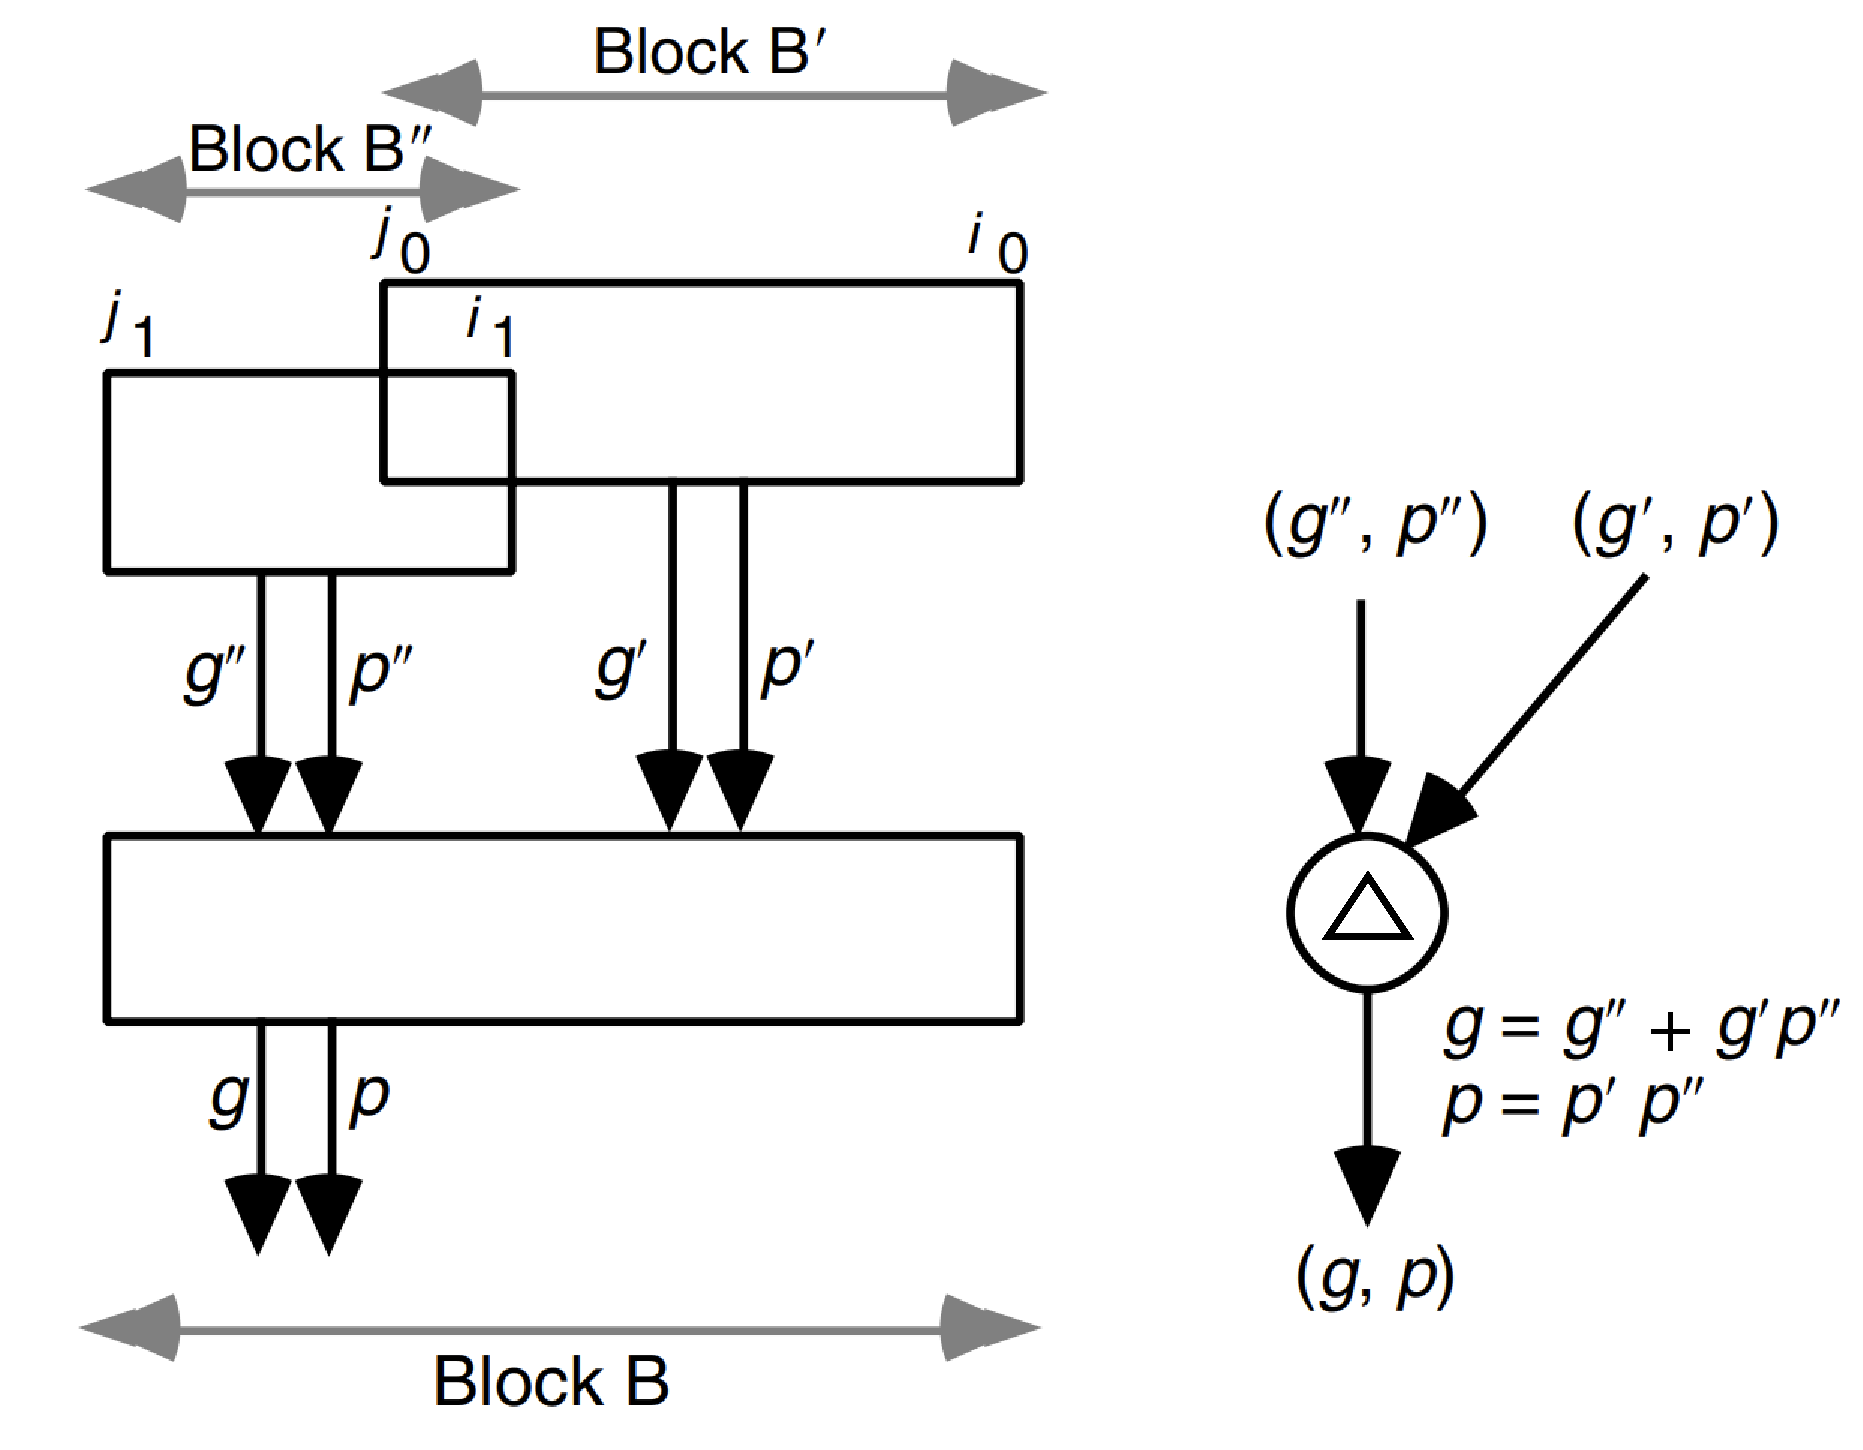
\includegraphics[width=0.6\textwidth]{figs/EM-PPA_BB.pdf}
    \caption{合并两个相邻或部分重叠的加法块$B \prime$、$B \prime \prime$的进位信号}
\label{EM:Fig:PPA_BB}
\end{figure}
如图\ref{EM:Fig:PPA_BB}所示,假设两个加法块$B \prime$和$B \prime \prime$相邻或重叠,则可以通过合并两对进位信号$(g \prime, p \prime)$和$(g \prime \prime, p \prime \prime)$来得到块$B$的进位信号$(g,p)$,假设该合并操作符号为$\triangle$,有:
\begin{equation}
    (g,p) = (g \prime, p \prime) \triangle (g \prime \prime, p \prime \prime)
\end{equation}
其中
\begin{align}
    g = \ & g \prime \prime + g \prime p \prime\prime \notag \\
    p = \ & p \prime p \prime \prime
\end{align}
注意$\triangle$满足结合律,不满足交换律:
\begin{align}
    ( \ (g \prime, p \prime) \triangle (g \prime \prime, p \prime \prime) \ ) \triangle (g \prime \prime \prime, p \prime \prime \prime) & \equiv (g \prime, p \prime) \triangle ( \ (g \prime \prime, p \prime \prime) \triangle (g \prime \prime \prime, p \prime \prime \prime) \ ) \notag \\
    (g \prime, p \prime) \triangle (g \prime \prime, p \prime \prime) & \not\equiv (g \prime \prime, p \prime \prime) \triangle (g \prime, p \prime)
\end{align}
这里假设块$B \prime \prime \prime$与块$B \prime \prime$相邻或重叠,进位信号为$(g \prime \prime \prime, p \prime \prime \prime)$。

基于此,可以定性地描述出进位问题:
假设加法器的位宽为$n$,给定$(g_0,p_0)$、$(g_1,p_1)$、$(g_2,p_2)$、$\cdots$、$(g_{n-1},p_{n-1})$,通过并行地计算
\begin{equation}
    (g_0,p_0) \triangle (g_1,p_1) \triangle (g_2,p_2) \triangle \cdots \triangle (g_{n-1},p_{n-1})
\end{equation}
能够得到所有的$(g_{[0,0]},p_{[0,0]})$、$(g_{[0,1]},p_{[0,1]})$、$(g_{[0,2]},p_{[0,2]})$、$\cdots$、$(g_{[0,n-1]},p_{[0,n-1]})$,即$c_1$、$c_2$、$c_3$、$\cdots$、$c_n$,且不同的并行方法对应不同的进位逻辑硬件实现,具有不同的面积和性能,称为并行前缀进位(Parallel Prefix Carry,PPC),得到的加法器被称为并行前缀加法器。
\begin{figure}[!htb]
    \centering
    \subfigure[超前进位加法器CLA的PPC树状图]{
    \label{EM:Fig:PPC_CLA}
    \begin{minipage}[t]{0.48\linewidth}
    \centering
    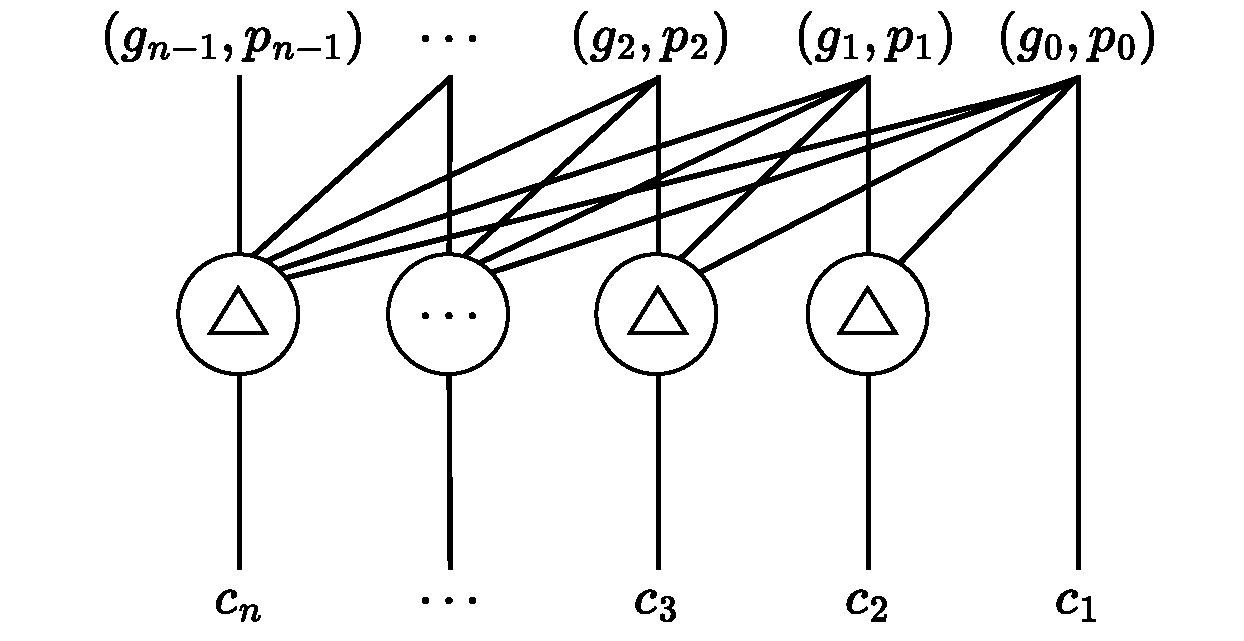
\includegraphics[width=\linewidth]{figs/EM-PPC_CLA.pdf}
    \end{minipage}
    }
    \subfigure[行波进位加法器RCA的PPC树状图]{
    \label{EM:Fig:PPC_RCA}
    \begin{minipage}[t]{0.48\linewidth}
    \centering
    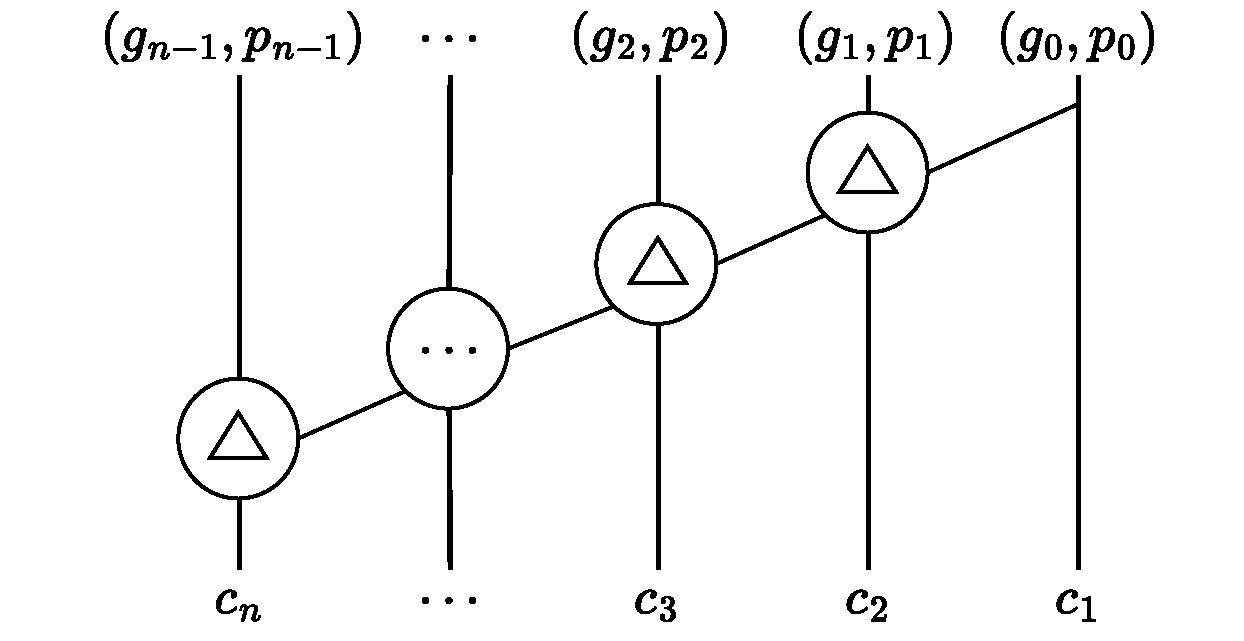
\includegraphics[width=\linewidth]{figs/EM-PPC_RCA.pdf}
    \end{minipage}
    }
\caption{标准CLA和标准RCA的PPC树状图}
\label{EM:Fig:PPC_CLA_RCA}
\end{figure}
PPC可由树状图进行表示,图\ref{EM:Fig:PPC_CLA_RCA}展示了标准超前进位加法器CLA和标准行波进位加法器RCA的PPC树状图。可以看到,CLA的PPC树状图只有一级,关键路径短,但计算量大;CLA的PPC树状图有$n$级,关键路径长,但使用了大量的中间节点,计算量小。因此,并行前缀加法器的核心在于如何权衡面积和延迟,这为并行前缀加法器的设计带来了非常大的灵活性\cite{EM:PPA_PPT}:
比如1960年的Sklansky加法器\cite{EM:Sklansky_adder},特点是级数少、扇出高;
1973年的Kogge-Stone加法器\cite{EM:Kogge-Stone_adder},优点是逻辑级数和扇出都非常小,缺点节点数量非常多,布线拥塞度高;
1980年的Ladner-Fisher加法器\cite{EM:Ladner-Fisher_adder},其结构与Sklansky加法器\cite{EM:Sklansky_adder}一致,原因是Ladner-Fischer形式化了进位问题的求解,Sklansky加法器是其中一种方案;
1982年的Brent-Kung加法器\cite{EM:Brent-Kung_adder},优点是扇出非常小,节点也较少,缺点是逻辑级数较多,即通过增加额外的逻辑级数来缓解扇出压力;
1987年的Han-Carlson加法器\cite{EM:Han-Carlson_adder},混合了Brent-Kung结构和Kogge-Stone结构,更有利于硬件实现;
1999年Knowles提出可以从逻辑深度、布线拥塞度和面积三个方面对进位网络的设计进行权衡\cite{EM:S-Knowles_adder};
2003年Harris提出了一个有趣的3-D结构图来对已有的并行前缀加法器进行分类\cite{EM:Harris_3-D},同时提出了一个新的进位结构;其余的前缀加法器包括Ling型加法器\cite{EM:Ling_adder}和具有多扇入节点的Beaumont-Smith加法器\cite{EM:Beaumont-Smith_adder}。
现代EDA(Electronic Design Automation)综合工具也往往根据用户约束来实现具有并行前缀结构的加法器。由于大位宽下并行前缀网络的搜索空间巨大,英伟达利用强化学习的方法设计出了面积更小、速度更快的加法器\cite{EM:PrefixRL};也有工作在观察到EDA流程中逻辑综合和物理综合的不统一后\cite{EM:PPA_Pareto},通过图神经网络的方式来进行优化\cite{EM:PPA_GNN}。

\section{对数乘法器} \label{对数乘法器}

1962年,John N. Mitchell提出了一个相当有趣的算法\cite{EM:mitchell}:在二进制下,可以通过加法来近似得到两个无符号非零定点数的乘积,最大误差不超过$\dfrac{1}{9}$,且编程实现非常简洁,原理如下:

% 设$m=0$,由式\eqref{EM:Eq:unsigned_fixed_Decimal}得两个$n$比特二进制无符号正整数$X$和$Y$的十进制值:, 

对于式\eqref{EM:Eq:unsigned_fixed_Binary},假设$R=2$、$m=0$,两个$n$比特二进制无符号整数$X$和$Y$:
\begin{equation}
    X = x_{n-1} x_{n-2} x_{n-3} \cdots x_1 x_0 \ \ \ \ \ \ \ \
    Y = y_{n-1} y_{n-2} y_{n-3} \cdots y_1 y_0 
\label{EM:Eq:mitchell_XY_binary}
\end{equation}
若$X$和$Y$均非零(正整数),有:
\begin{align}
    x_{n-1} + x_{n-2} + x_{n-3} + \cdots + x_1 + x_0 = 1 \notag \\
    y_{n-1} + y_{n-2} + y_{n-3} + \cdots + y_1 + y_0 = 1
\end{align}
则$X$和$Y$的十进制值为:
\begin{align}
    V(X) = \sum_{i=0}^{k_X} x_i 2^i \ \ \ \ \ \ \ \ \ \ \ \ \ \ \ 
    V(Y) = \sum_{i=0}^{k_Y} y_i 2^i
\end{align}
其中$k_X$和$k_Y$分别代表$X$和$Y$中最高位的1的权重值\cite{AC:AM:TOSAM},乘积$P$的十进制值:
\begin{align}
    V(P) = & \ V(X)V(Y) \notag \\
    = & \ \sum_{i=0}^{k_X} x_i 2^i \times \sum_{i=0}^{k_Y} y_i 2^i \notag \\
    = & \ 2^{k_X} ( \ 1 + \sum_{i=0}^{k_X - 1} x_i 2^{i-k_X} \ ) \times 2^{k_Y} ( \ 1 + \sum_{i=0}^{k_Y - 1} y_i 2^{i-k_Y} \ ) \notag \\
    = & \ 2^{k_X + k_Y} ( \ 1 + \sum_{i=0}^{k_X - 1} x_i 2^{i-k_X} \ ) ( \ 1 +  \sum_{i=0}^{k_Y - 1} y_i 2^{i-k_Y}\ ) \notag \\
    = & \ 2^{k_X + k_Y} ( \ 1 + x^{\prime} \ ) ( \ 1 + y^{\prime} \ )
\label{EM:Eq:mitchell_P_orig}
\end{align}
其中
\begin{equation}
    x^{\prime} = \sum_{i=0}^{k_X - 1} x_i 2^{i-k_X} \ \ \ \ \ \ \ \
    y^{\prime} = \sum_{i=0}^{k_Y - 1} y_i 2^{i-k_Y}
\end{equation}
则:
\begin{equation}
    \log_2 (V(P)) = k_X + k_Y + \log_2 (1+x^{\prime}) + \log_2 (1+y^{\prime})
\label{EM:Eq:mitchell_log_P}
\end{equation}
易知$x, y \in [0,1)$,在这里,Mitchell做了一个相当果断而美妙的近似,那就是利用$\log_2 (1+x^{\prime}) \approx x^{\prime}$和$\log_2 (1+y^{\prime}) \approx y^{\prime}$将式\eqref{EM:Eq:mitchell_log_P}变为:
\begin{equation}
    \log_2 (V(P)) \approx k_X + k_Y + x^{\prime} + y^{\prime}
\label{EM:Eq:mitchell_log_P_2}
\end{equation}
则乘积$P$:
\begin{equation}
    V(P) \approx 2^{(k_X + k_Y)} \cdot 2^{(x^{\prime} + y^{\prime})}
\label{EM:Eq:mitchell_P_middle}
\end{equation}
这里再做一次近似:
\begin{equation}
    x^{\prime} + y^{\prime} \approx \left\{
    \begin{aligned}
        \ & \log_2 (1 + x^{\prime} + y^{\prime}) , & \ \ x^{\prime} + y^{\prime} < 1, \\
        \ & 1 + \log_2 (x^{\prime} + y^{\prime}), & \ \ x^{\prime} + y^{\prime} \ge 1.
    \end{aligned}
    \right.
\end{equation}
则式\eqref{EM:Eq:mitchell_P_middle}变为:
\begin{equation}
    V(P) \approx \left\{
    \begin{aligned}
        \ & 2^{(k_X + k_Y)} (1 + x^{\prime} + y^{\prime}) , & \ \ x^{\prime} + y^{\prime} < 1, \\
        \ & 2^{(k_X + k_Y + 1)} (x^{\prime} + y^{\prime}), & \ \ x^{\prime} + y^{\prime} \ge 1.
    \end{aligned}
    \right.
\label{EM:Eq:mitchell_P_final}
\end{equation}
式\eqref{EM:Eq:mitchell_P_final}即为Mitchell对数乘法器的最终形式,只需要加法、移位和检测电路即可完成两数相乘,可以证明Mitchell算法的最大误差不超过精确值的$\dfrac{1}{9}$。

在C++中,Mitchell算法有一个非常简单的实现\footnote{https://kexue.fm/archives/7991},单精度(Single precision)浮点数运算的代码如算法\ref{EM:Alg:mitchell_Cpp}所示\cite{DNN:mitchell_Training},原理如下:

\begin{algorithm}[!]
    float int mitchell\_mul (const float a, const float b) \{ \\
    \ \ \ \ \ \ \ \ int c = *(int*)\&a + *(int*)\&b - 0x3f800000; \\
    \ \ \ \ \ \ \ \ return *(float*)\&c; \\
    \}
\caption{Mitchell算法在C++中的简单实现}
\label{EM:Alg:mitchell_Cpp}
\end{algorithm}

C++中int类型通常是32位,同时IEEE 754标准规定采用32个比特表示单精度浮点数,如图\ref{EM:Fig:mitchell_IEEE754}所示,其中最高位表示正负,之后8位表示科学计数法的指数,最后23位表示科学计数法的小数,注意指数部分需要加上偏移量127。对于两个单精度浮点数a和b,*(int*)\&a和*(int*)\&b其实就是把a和b对应的二进制表示拿出来,当作普通的int类型将两者相加,对应式\eqref{EM:Eq:mitchell_log_P_2},这时指数部分还多出一个偏移量,所以要减去这个偏移量,由于偏移量是127,并且后面还有23位,所以要减去常数$127×2^{23}$,十六进制为0x3f800000,最后将结果恢复为单精度浮点数。对双精度(Double precision)浮点数来说,在引入64比特位宽的long int类型和正确的偏移量($1023 \times 2^{52} = \text{0x3feffffb9f6e8000}$)之后,算法\ref{EM:Alg:mitchell_Cpp}同样适用(已验证)。

\begin{figure}[!htb]
    \centering
    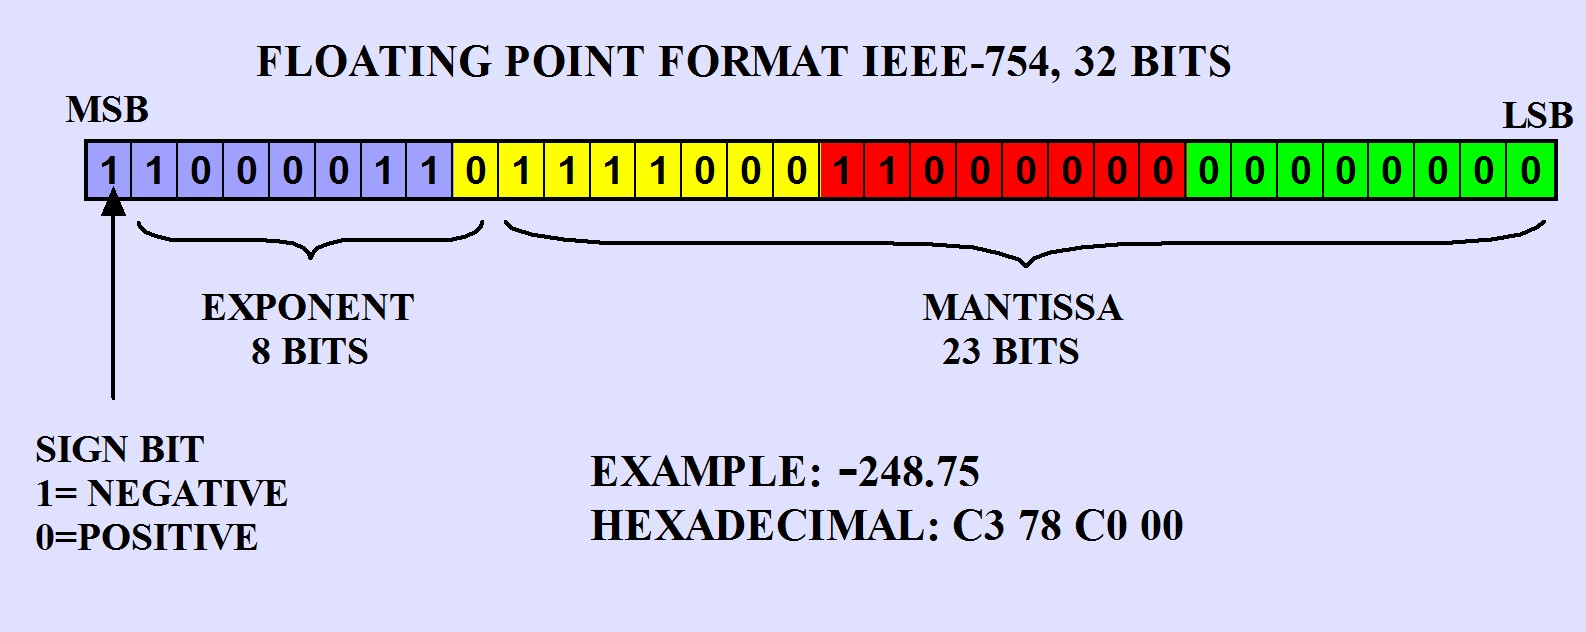
\includegraphics[width=0.8\linewidth]{figs/EM-mitchell_IEEE754.jpg}
    \caption{IEEE 754单精度浮点数标准}
    \label{EM:Fig:mitchell_IEEE754}
\end{figure}

Mitchell算法能够将乘法近似转化为加法实现,这对需要大量乘法并对误差有容忍性的神经网络应用带来了计算量优化的可能,比如有篇NeurIPS 2020的工作便在“ImageNet+ResNet50”中直接将神经网络中的乘法换成Mitchell近似的加法形式,准确率只有轻微的下降,甚至可能不下降\cite{DNN:mitchell_Training},而这也并不是Mitchell近似在深度学习中第一次被讨论\cite{AC:AM:mitchell_aspdac2018,AC:AM:mitchell_tc2019}。

\section{近似电路的误差指标} \label{近似电路的误差指标}

近似电路通常是指近似的算术单元,如加法器、减法器、乘法器、除法器等,这些近似模块在计算中可能会产生误差,用来衡量误差的最基本的两个指标分别是误差率(Error Rate,ER)和误差距离(Error Distance,ED)\cite{AC:Arith:survey_hanjie}。ER表示产生错误结果的概率,ED代表近似结果和精确结果之间的算术差异。假设在某输入下近似电路的结果是$M \prime$,精确电路的结果是$M$,那么该输入下误差距离为:
\begin{equation}
    ED = | M′−M |
\label{AC:Arith:ED}
\end{equation}
相对误差距离(Relative ED,RED)表示近似结果与准确结果的相对算术差异,则
\begin{equation}
    RED = \dfrac{ED}{M}
\label{AC:Arith:RED}
\end{equation}
ED和RED是衡量近似电路在某输入下误差的两个重要指标。

当考虑所有的输入情况时,可由平均误差距离(Mean ED,MED)和平均相对误差距离(Mean RED,MRED)来衡量近似电路和精确电路之间的整体算术差异,MED和MRED被定义为:
\begin{align}
    & MED = \sum _{i=1}^{N} ED_{i} \cdot P(ED_{i}) \label{AC:Arith:MED} \\
    & MRED = \sum _{i=1}^{N} RED_{i} \cdot P(RED_{i}) \label{AC:Arith:MRED}
\end{align}
其中$N$是所有输入情况的总数,$ED_{i}$和$RED_{i}$分别代表输入是第$i$种情况下的误差距离ED和相对误差距离RED,$P(ED_{i})$和$P(RED_{i})$分别代表$ED_{i}$和$RED_{i}$发生的概率,即输入取第$i$种情况的概率。MED也被叫做平均绝对误差(Mean Absolute Error,MAE)。
归一化平均误差距离(Normalized MED,NMED)被定义为MED除以精确电路在所有输入情况下的最大值,常被用来比较同一近似设计方法在不同输入位宽下的误差表现。

均方误差(Mean Squared Error,MSE)和均方根误差(Root MSE,RMSE)也被广泛用于衡量近似电路和精确电路之间的算术误差幅度,它们被定义为:
\begin{align}
    & MSE = \sum _{i=1}^{N}ED_{i}^{2}\cdot P(ED_{i}) \label{AC:Arith:MSE} \\
    & RMSE = \sqrt {MSE} \label{AC:Arith:RMSE}
\end{align}
另外,平均误差被定义为所有可能输入情况下$M \prime - M$的平均值,归一化平均误差被定义为平均误差除以精确电路在所有输入情况下的最大值。最后,最坏情况误差(Worst Case Error,WCE)反映了可能的最大ED。

以上提到的衡量近似电路误差的指标均适用于近似乘法器。

\section{本章小结}

本章首先介绍了精确定点数乘法器的三个运算过程:部分积的生成、累加、最终相加,以及针对每个过程不同的实现方法。其中,无符号数相乘的部分积可由与门直接产生,补码有符号数乘法的部分积根据设计方法的不同有多种生成办法,目前使用最广泛的产生方式是基于Baugh-Wooley算法和基4的布斯算法;对部分积的累加来讲,通过将全加器排列为树形,并采用进位保存的思想可得到较为高速的累加阵列;累加结束后的部分积数量减少为2个,需要一个多位宽的向量加法器完成最终相加,可根据需求选择行波进位加法器、超前进位加法器、进位选择加法器、并行前缀加法器等不同结构完成最终结果的计算。本章紧接着介绍了由Mitchell发明的对数乘法器,该乘法器可将乘法转变为加法,大大降低了计算量,误差最大不超过$\dfrac{1}{9}$;最后介绍了用来衡量近似电路误差的不同指标,这些指标适用于常见的近似算术单元。